\section{安定化制御実験}
	振子を上向きに配置したときに安定化制御が可能か実験を行う。(実験目的の第一項目)
	その際に、振子を真上に配置するのではなく、幾分か角度をつけてから実験を始める。
	実験に用いたパラメータを以下の表に示す。
	\begin{table}[htb]
		\begin{center}
			\caption{安定化制御実験で使用したパラメータの組}
			\medskip
			
			\begin{tabular}{|c|c|c|c|}\hline
				重み行列$Q$ & オブザーバの極$P$ & サンプリング周期$\Delta[\rm{s}]$ \\ \hline\hline
				$Q_1$:$\rm{diag}(1E5,1E5,1,1)$ & $P_1$:$((-30,0),(-30,0))^{'}$ & $\Delta_1$:0.005 \\ \hline
			\end{tabular}
		\end{center}
		\label{table:huriage_control}
	\end{table}
	以下に実験結果とシミュレーション結果の比較図を示す。
	\begin{figure}[H]
		\centering
		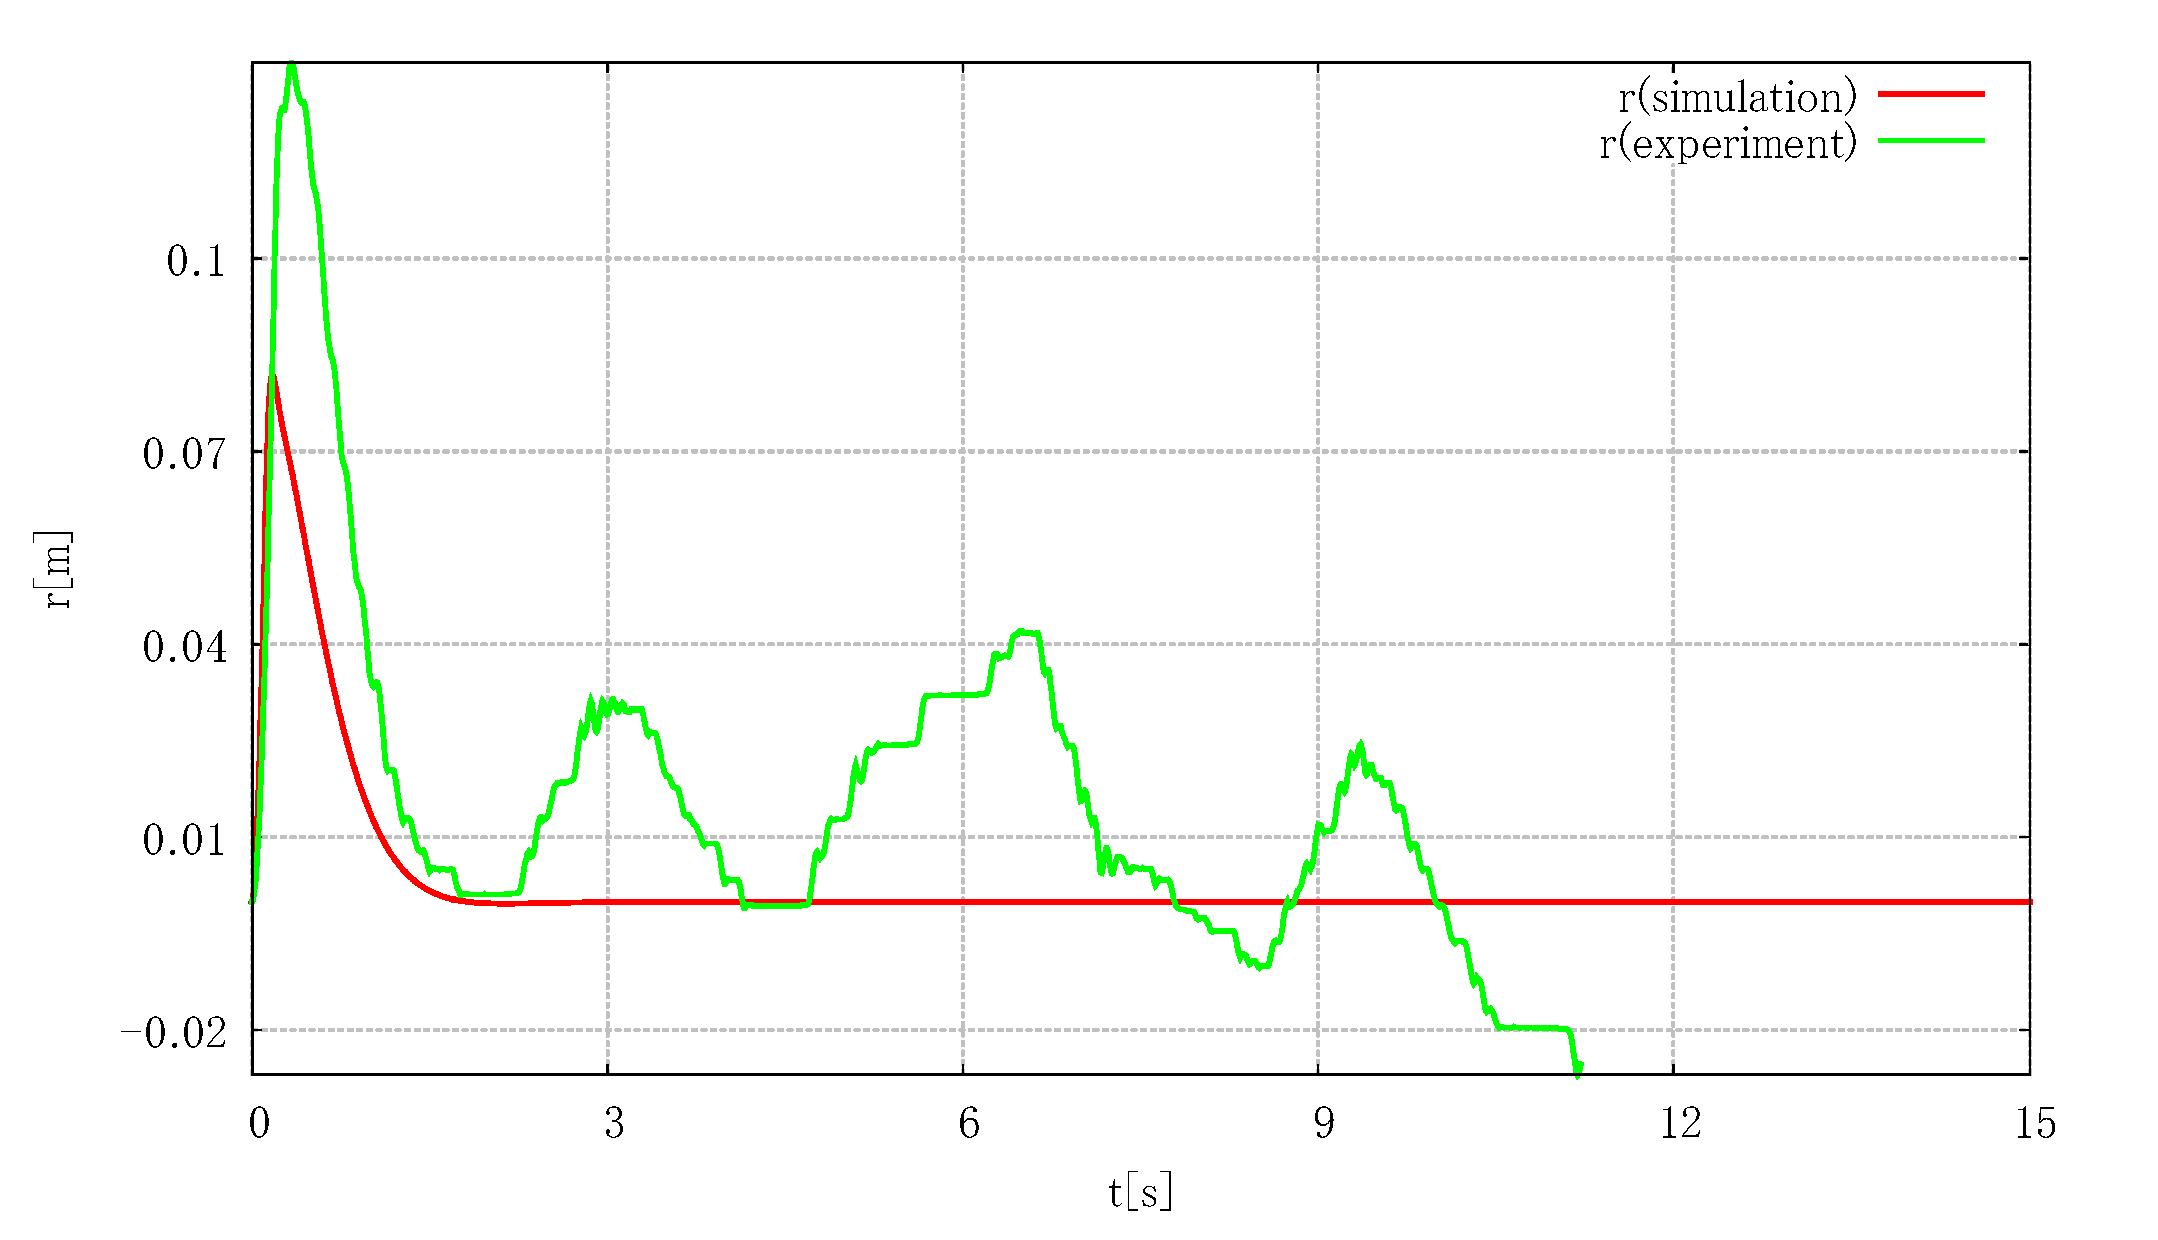
\includegraphics[width=0.8\linewidth]{gazo/experiment_control_R.eps}
		\caption{安定化制御実験結果(台車位置)}
		\label{image:experiment_control_R}
	\end{figure}
	\begin{figure}[H]
		\centering
		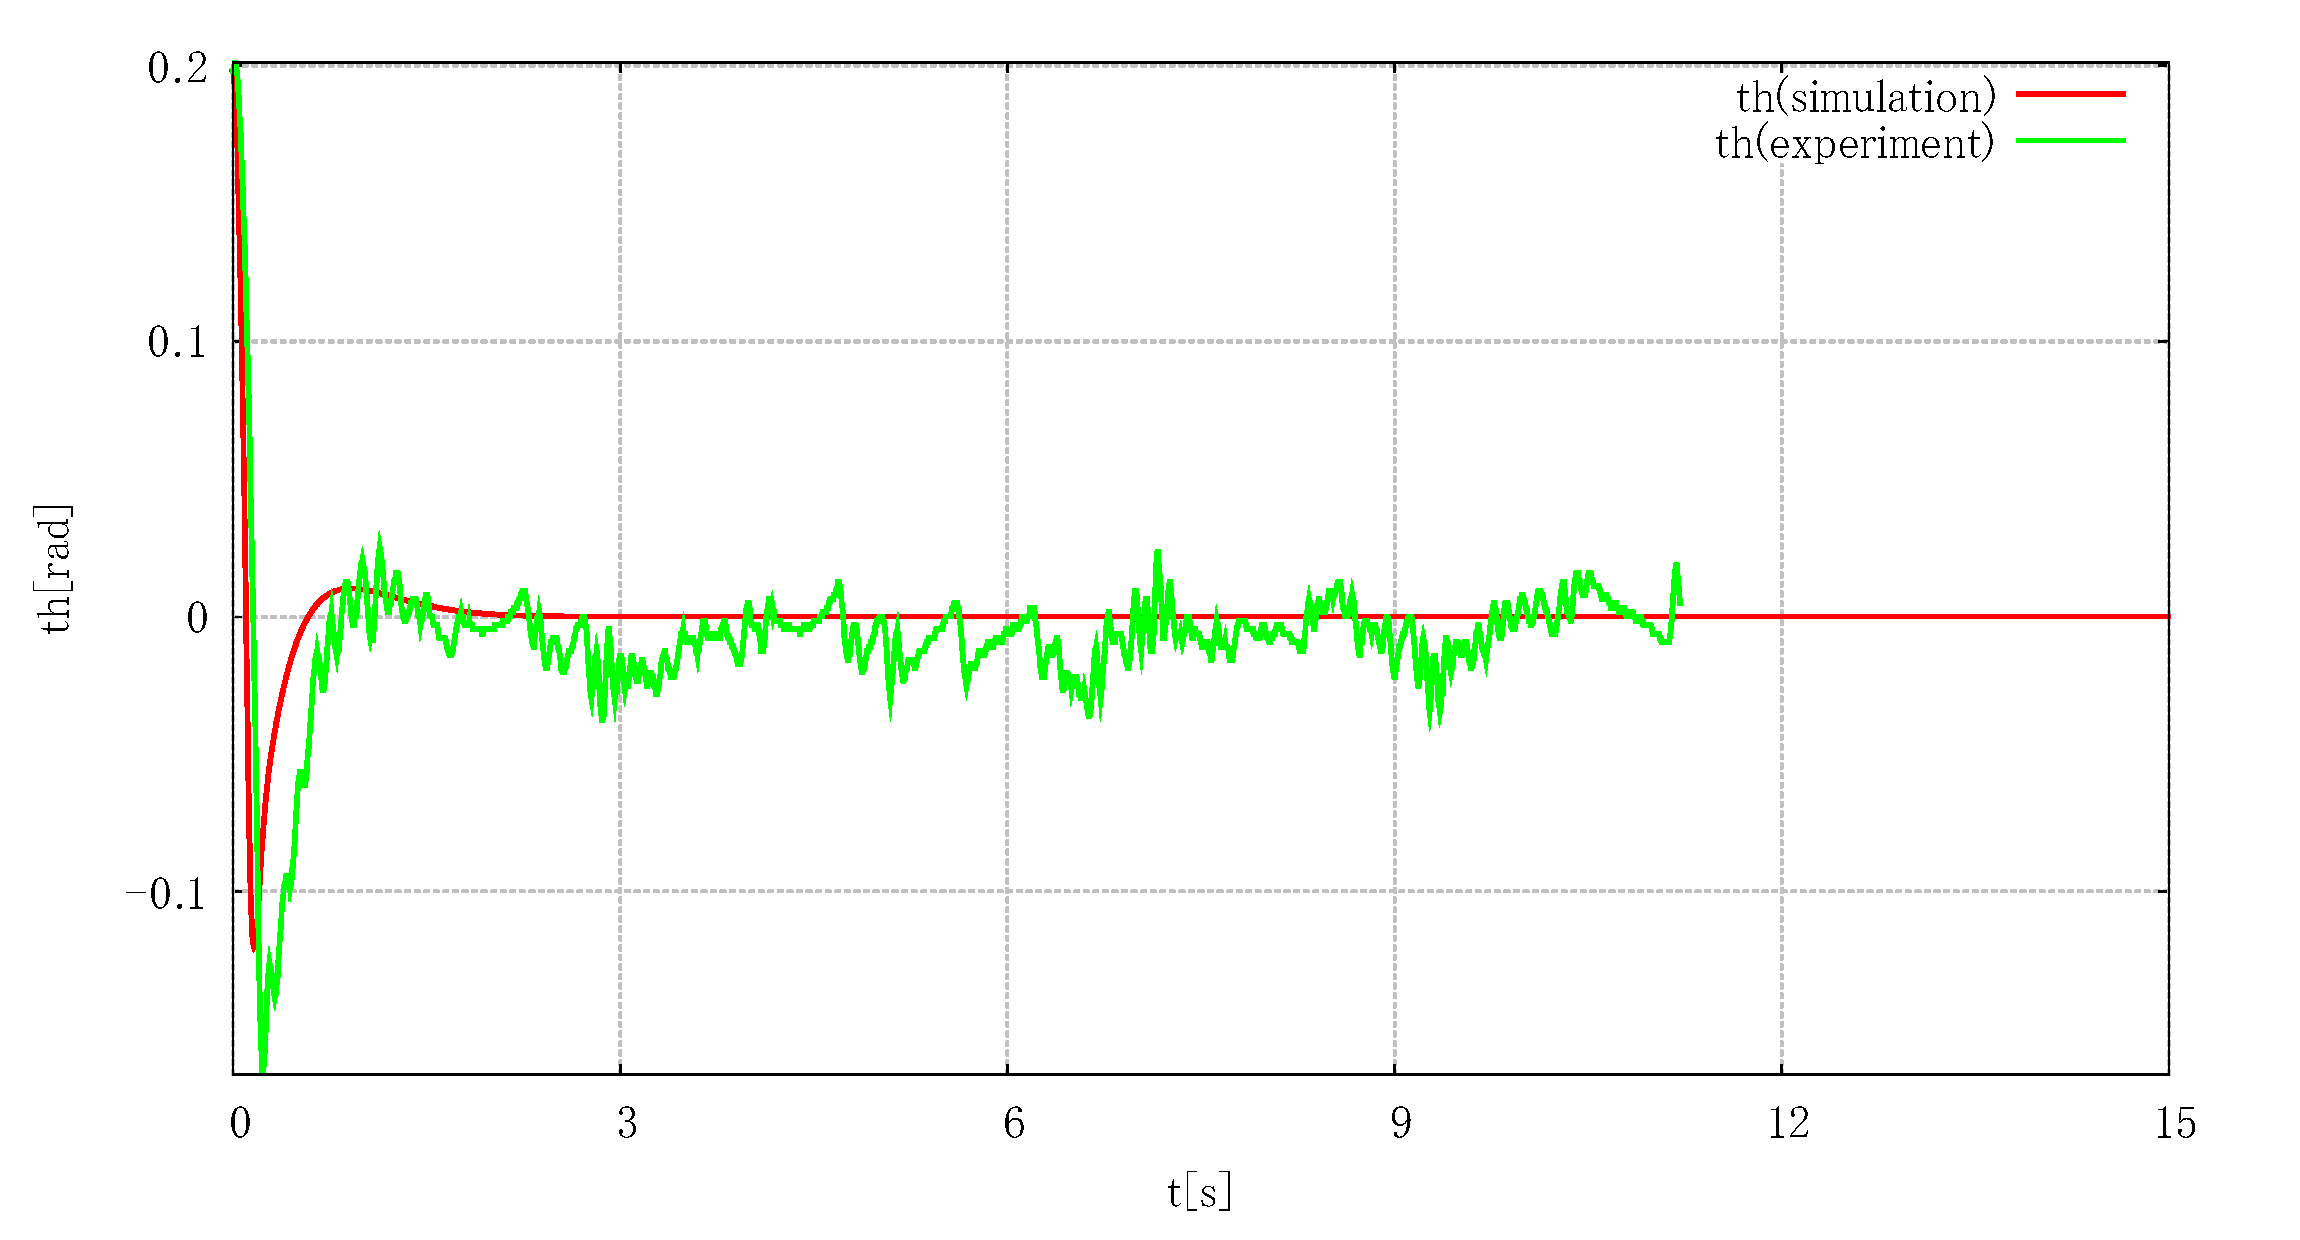
\includegraphics[width=0.8\linewidth]{gazo/experiment_control_TH.eps}
		\caption{安定化制御実験結果(振子角度)}
		\label{image:experiment_control_TH}
	\end{figure}
	図\ref{image:experiment_control_R}と図\ref{image:experiment_control_TH}
	より一番最初の山は実験のほうが大幅に大きくなっているのと、ノイズが乗っている点を除いてシミュレーションと実験結果は
	概ね一致しているといえる。これは、実験のほうではデータの計測を開始して振子から手を離したためその影響が出たといえる。
	この時の初期角度は$0.1979°$である。%radに直してほしいなぁ
	よって、初期角度がある程度ある中で実験を開始し、安定化制御を行うことができたため、
	実験目的の第一項目を達成できたといえる。
	
	
	
%-----------------------------------------------------------
\section{目標値の変更実験}
	台車に目標値を与えて、その目標値に台車が移動しても安定化制御可能か実験を行う。(実験項目の第二項目)
	なお、目標値は5秒ごとに0→0.1→0のように変更される。
	以下に、重み行列を変更した場合の比較、オブザーバの極を変更した場合の比較、サンプリング周期を変更した場合の比較を
	行った図を示す。
	%JAMOXで3種の図を作成
	%貼り付ける
	%考察を述べる
	以下に実験結果とシミュレーション結果との比較を行った図を示す。
	図の数が多いので図のキャプションとその図における各パラメータの対応表を示す。
	\begin{table}[htb]
		\begin{center}
			\caption{図に対応するパラメータの組}
			\medskip
			
			\begin{tabular}{|c|c|c|c|}\hline
				図のキャプション & 重み行列$Q$ & オブザーバの極$P$ & サンプリング周期$\Delta[\rm{s}]$ \\ \hline\hline
				比較結果その1 & $Q_1$:$\rm{diag}(1E5,1E5,1,1)$ & $P_1$:$((-30,0),(-30,0))^{'}$ & $\Delta_1$:0.005 \\ \hline
				比較結果その2 & $Q_1$:$\rm{diag}(1E5,1E6,1,1)$ & $P_1$:$((-30,0),(-30,0))^{'}$ & $\Delta_1$:0.005 \\ \hline
				比較結果その3 & $Q_1$:$\rm{diag}(1E6,1E5,1,1)$ & $P_1$:$((-30,0),(-30,0))^{'}$ & $\Delta_1$:0.005 \\ \hline
				比較結果その4 & $Q_1$:$\rm{diag}(1E5,1E5,1,1)$ & $P_1$:$((-60,0),(-30,0))^{'}$ & $\Delta_1$:0.005 \\ \hline
				比較結果その5 & $Q_1$:$\rm{diag}(1E5,1E6,1,1)$ & $P_1$:$((-60,0),(-30,0))^{'}$ & $\Delta_1$:0.005 \\ \hline
				比較結果その6 & $Q_1$:$\rm{diag}(1E6,1E5,1,1)$ & $P_1$:$((-60,0),(-30,0))^{'}$ & $\Delta_1$:0.005 \\ \hline
				比較結果その7 & $Q_1$:$\rm{diag}(1E5,1E5,1,1)$ & $P_1$:$((-30,0),(-30,0))^{'}$ & $\Delta_1$:0.010 \\ \hline
				比較結果その8 & $Q_1$:$\rm{diag}(1E5,1E6,1,1)$ & $P_1$:$((-30,0),(-30,0))^{'}$ & $\Delta_1$:0.010 \\ \hline
				比較結果その9 & $Q_1$:$\rm{diag}(1E6,1E5,1,1)$ & $P_1$:$((-30,0),(-30,0))^{'}$ & $\Delta_1$:0.010 \\ \hline
				比較結果その10 & $Q_1$:$\rm{diag}(1E5,1E5,1,1)$ & $P_1$:$((-60,0),(-30,0))^{'}$ & $\Delta_1$:0.010 \\ \hline
				比較結果その11 & $Q_1$:$\rm{diag}(1E5,1E6,1,1)$ & $P_1$:$((-60,0),(-30,0))^{'}$ & $\Delta_1$:0.010 \\ \hline
				比較結果その12 & $Q_1$:$\rm{diag}(1E6,1E5,1,1)$ & $P_1$:$((-60,0),(-30,0))^{'}$ & $\Delta_1$:0.010 \\ \hline
			\end{tabular}
		\end{center}
		\label{table:huriage_control}
	\end{table}
	
	\begin{figure}[H]
		\centering
		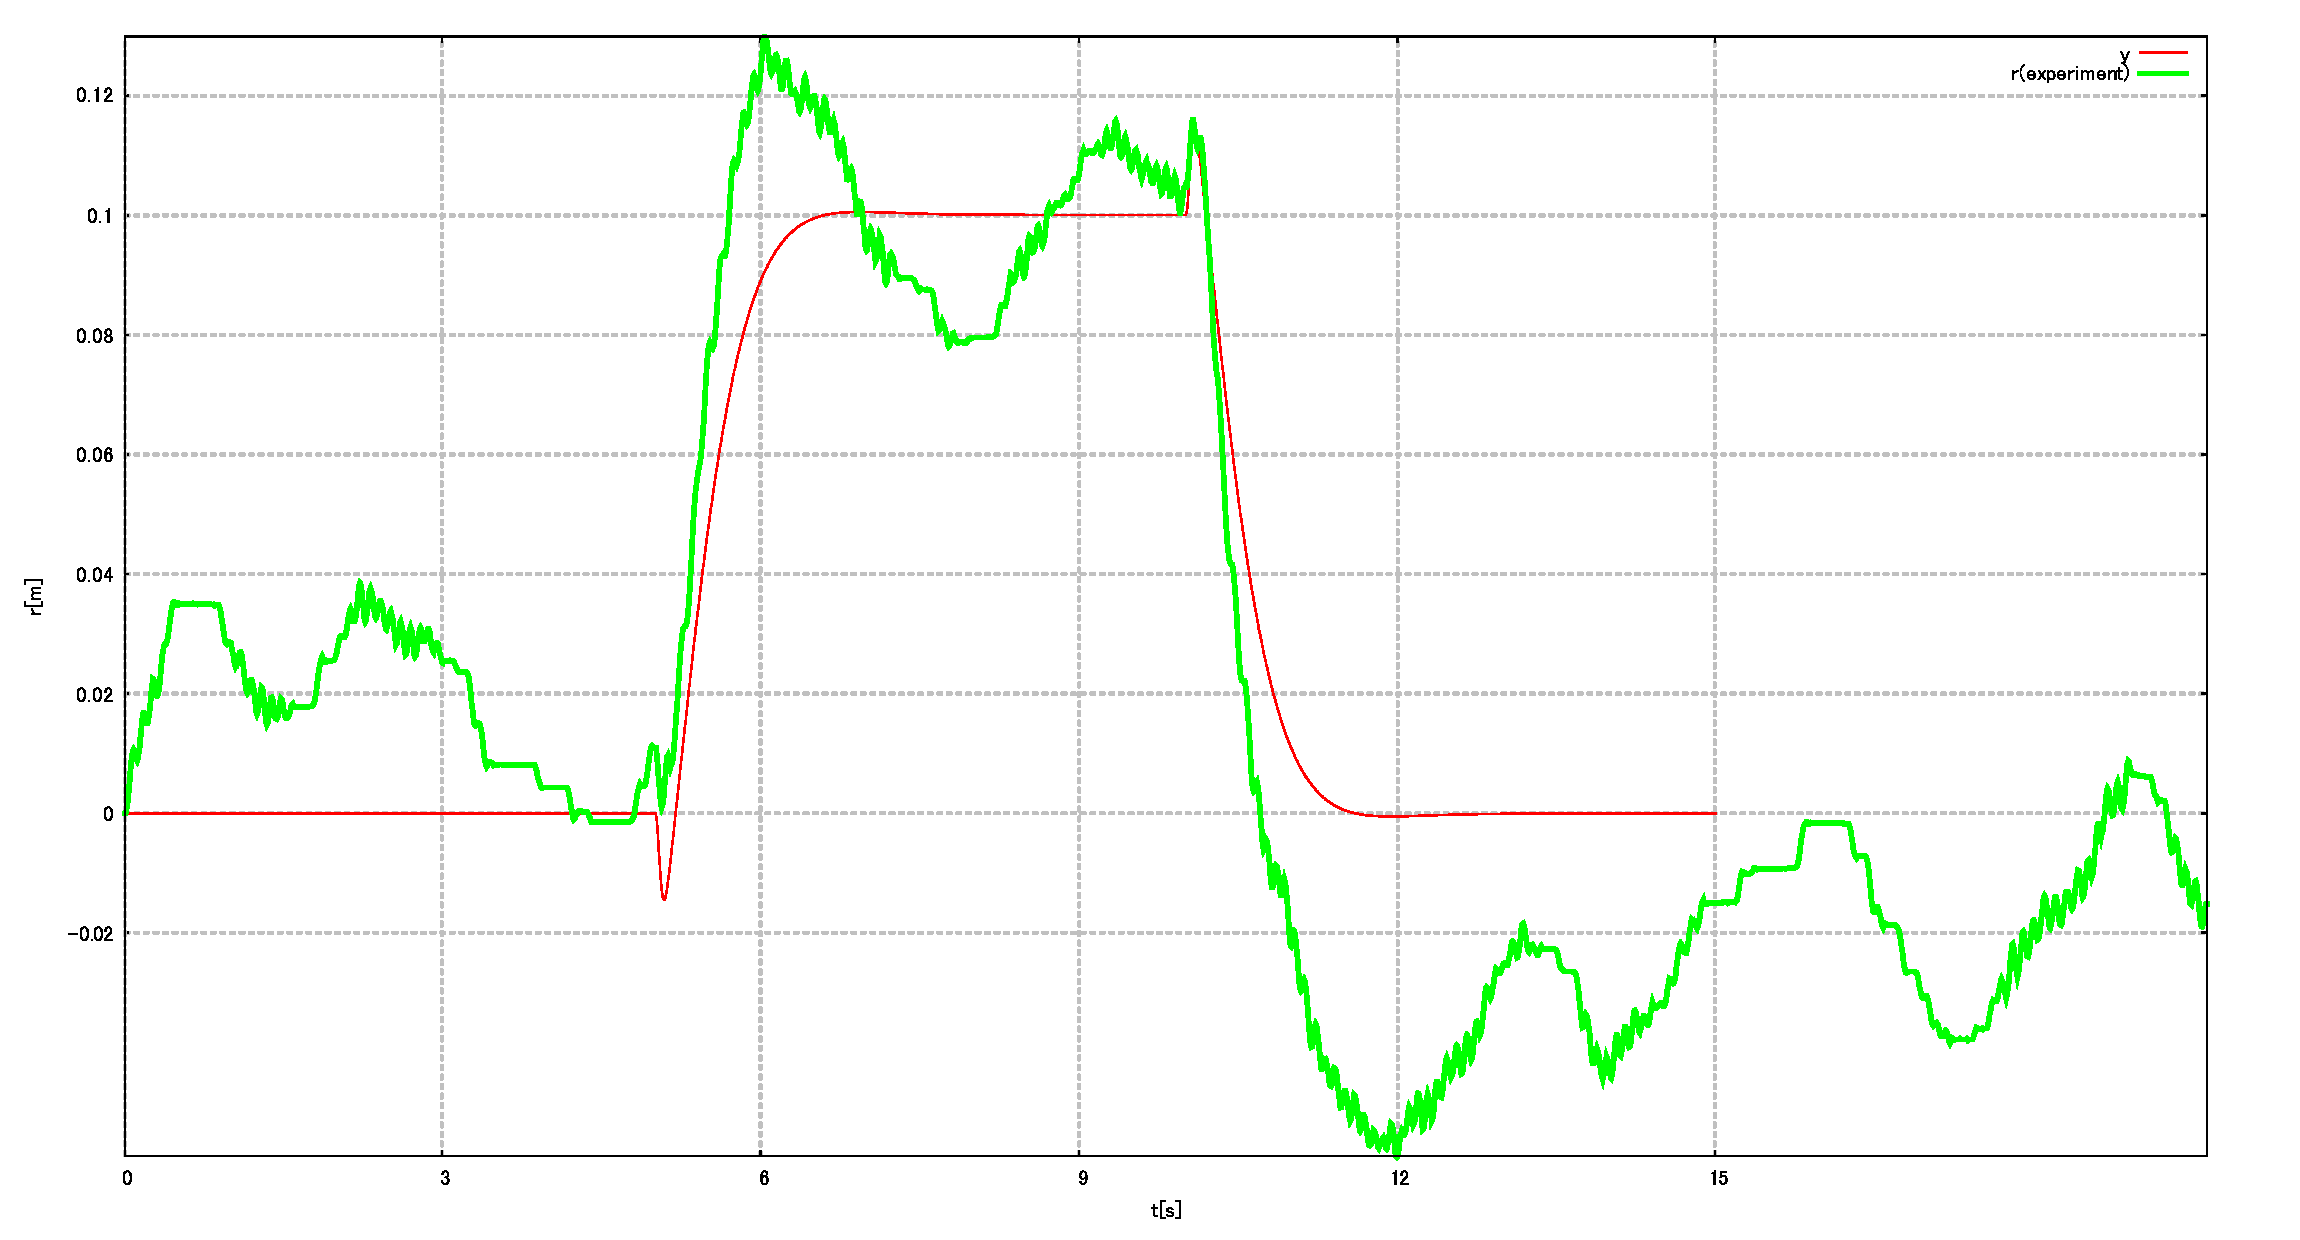
\includegraphics[width=0.4\linewidth]{gazo/experiment_Q55obs30dt05R.eps}
		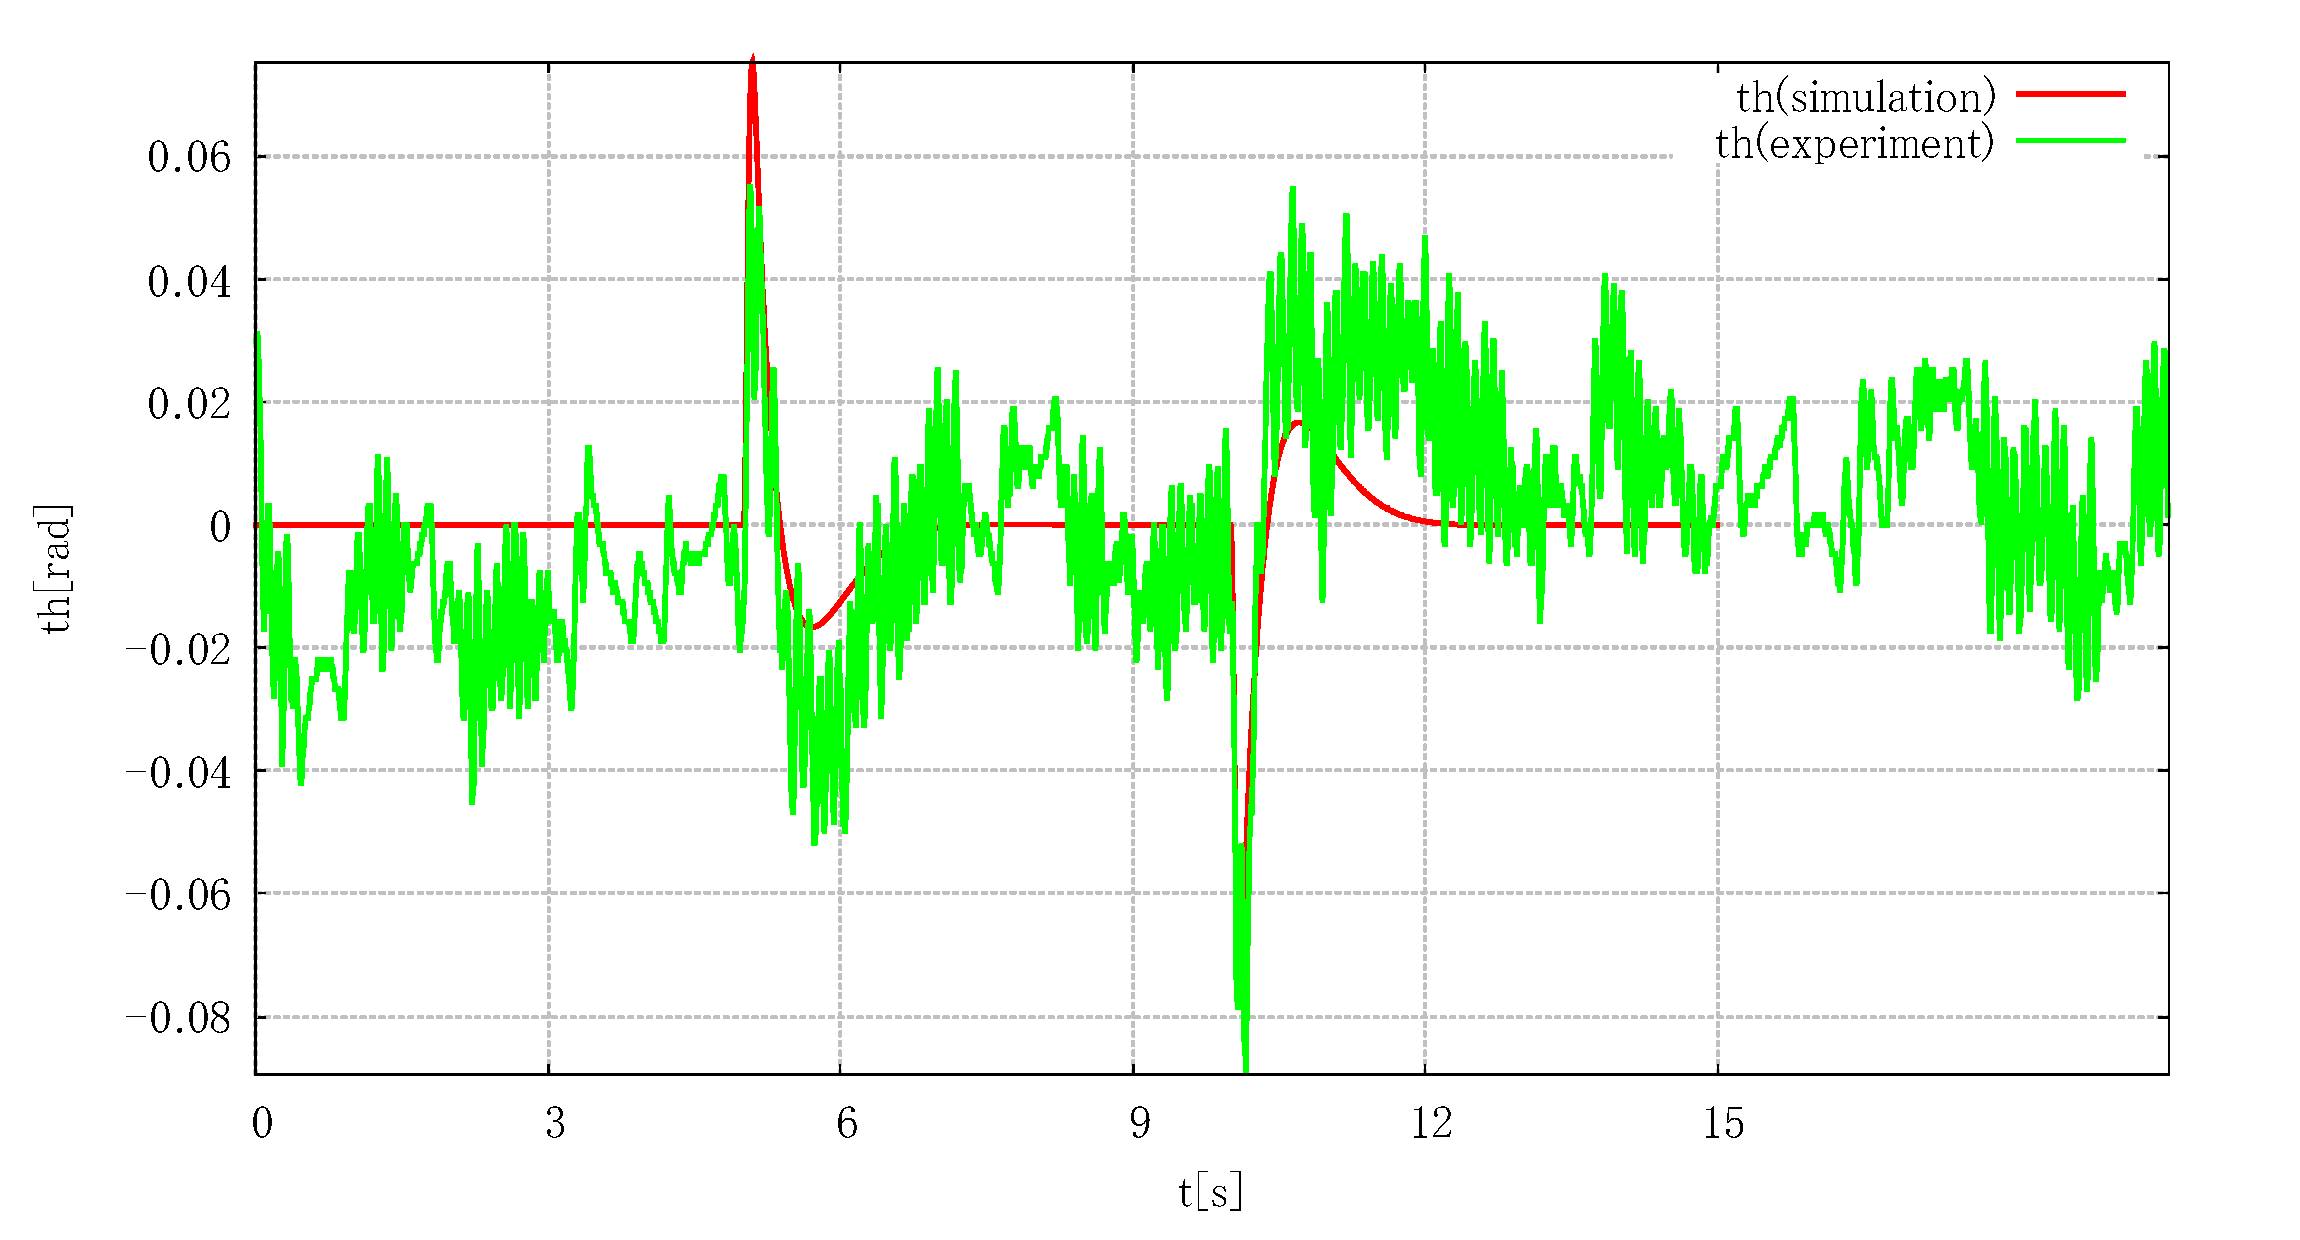
\includegraphics[width=0.4\linewidth]{gazo/experiment_Q55obs30dt05TH.eps}
		\caption{比較結果その1(左図がr,右図が$\theta$)}
		\label{image:sono1}
	\end{figure}
	\begin{figure}[H]
		\centering
		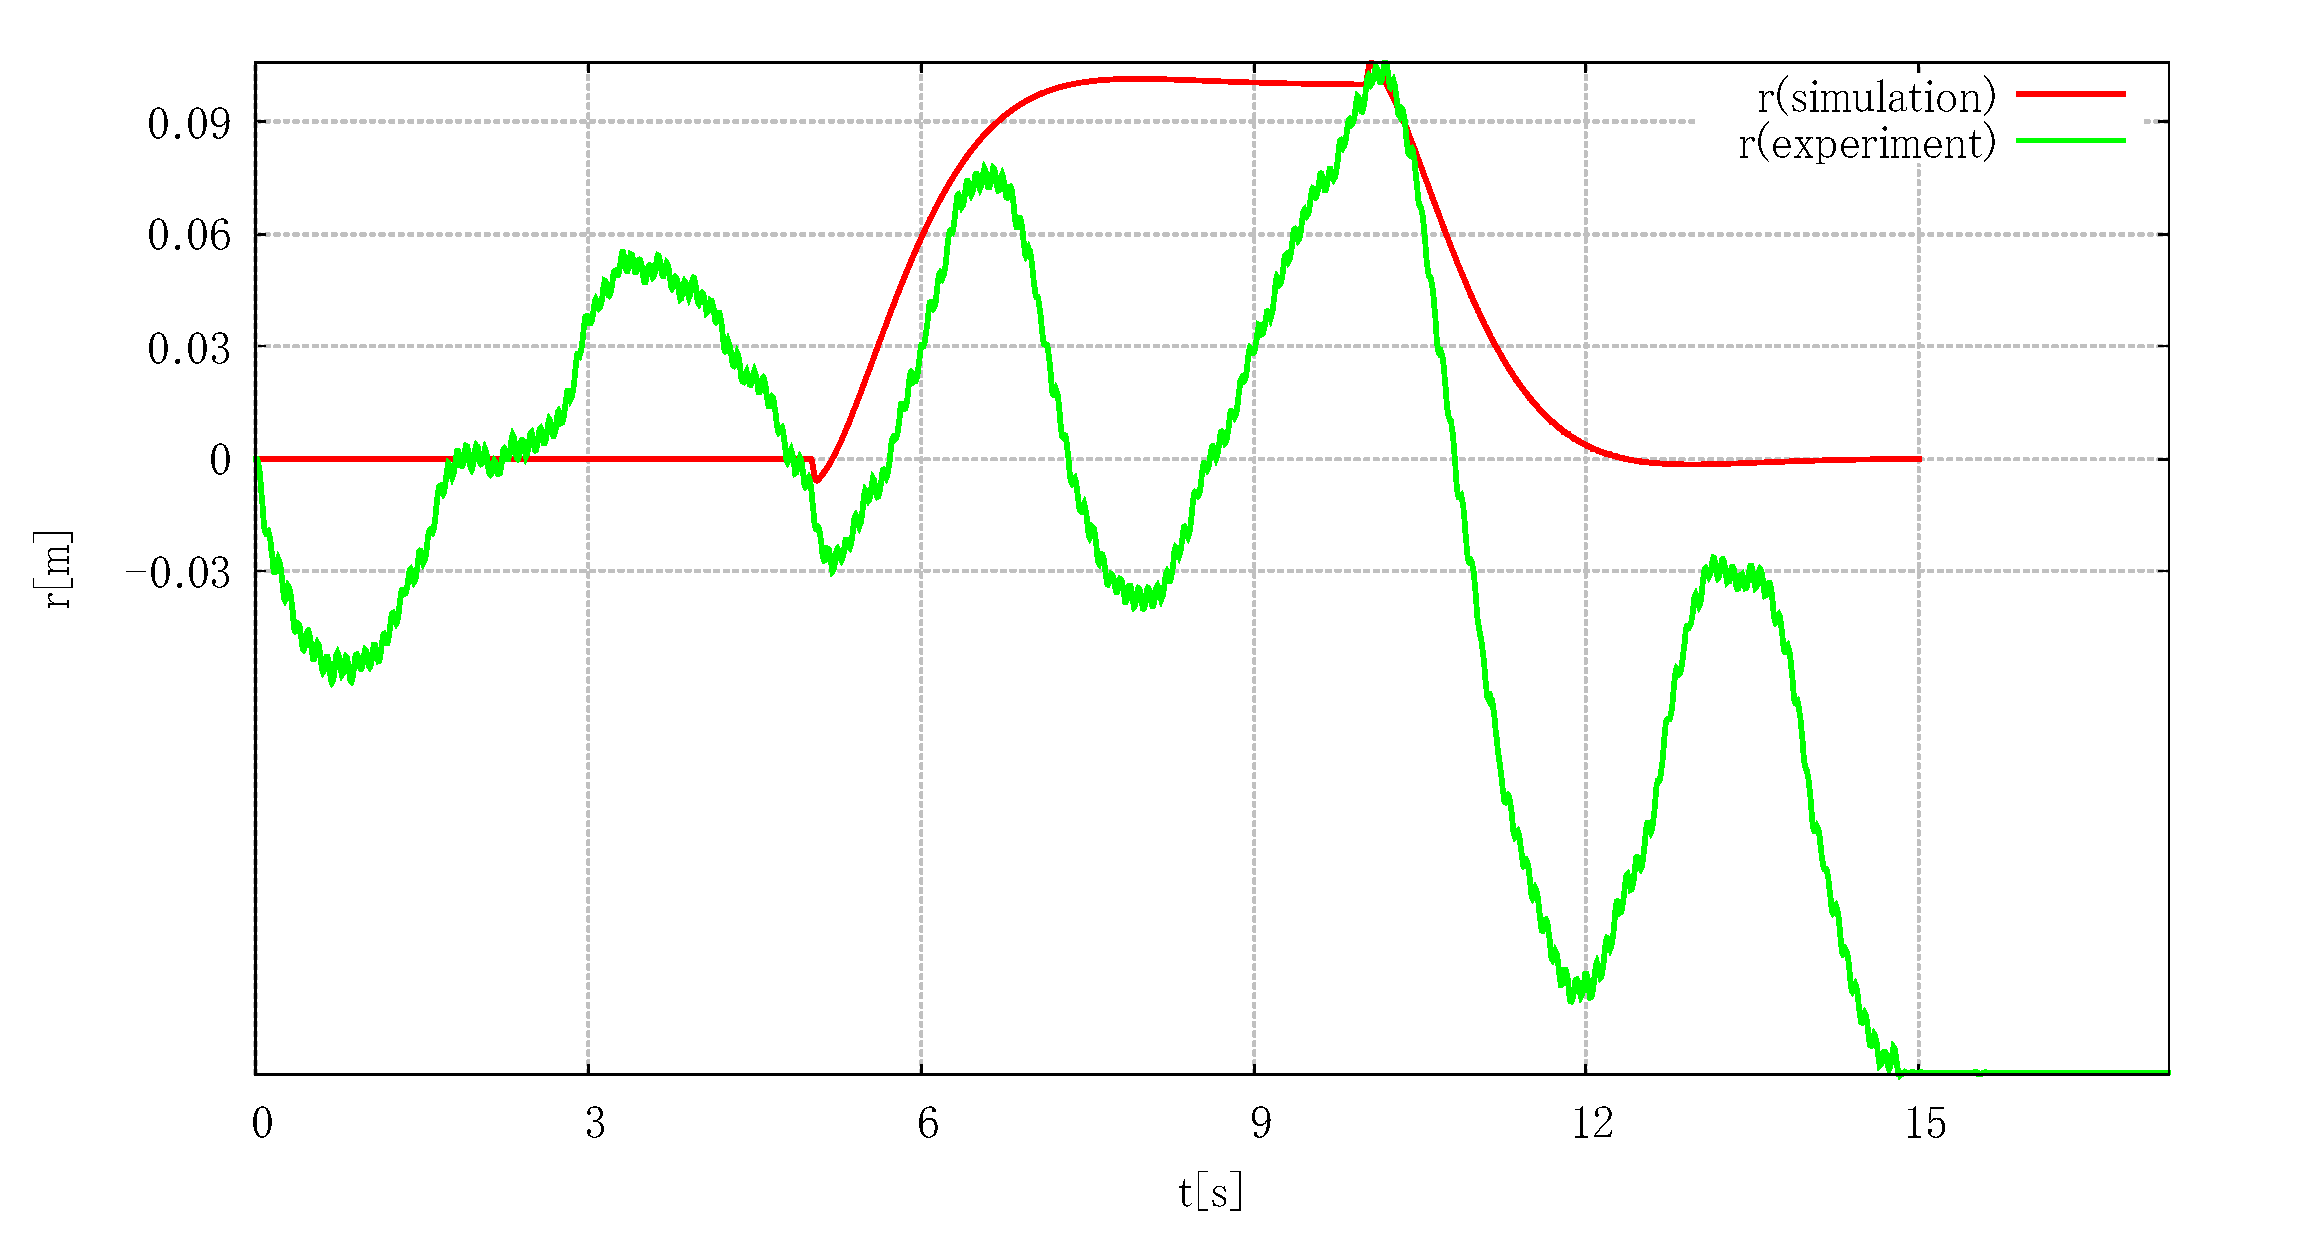
\includegraphics[width=0.4\linewidth]{gazo/experiment_Q56obs30dt05R.eps}
		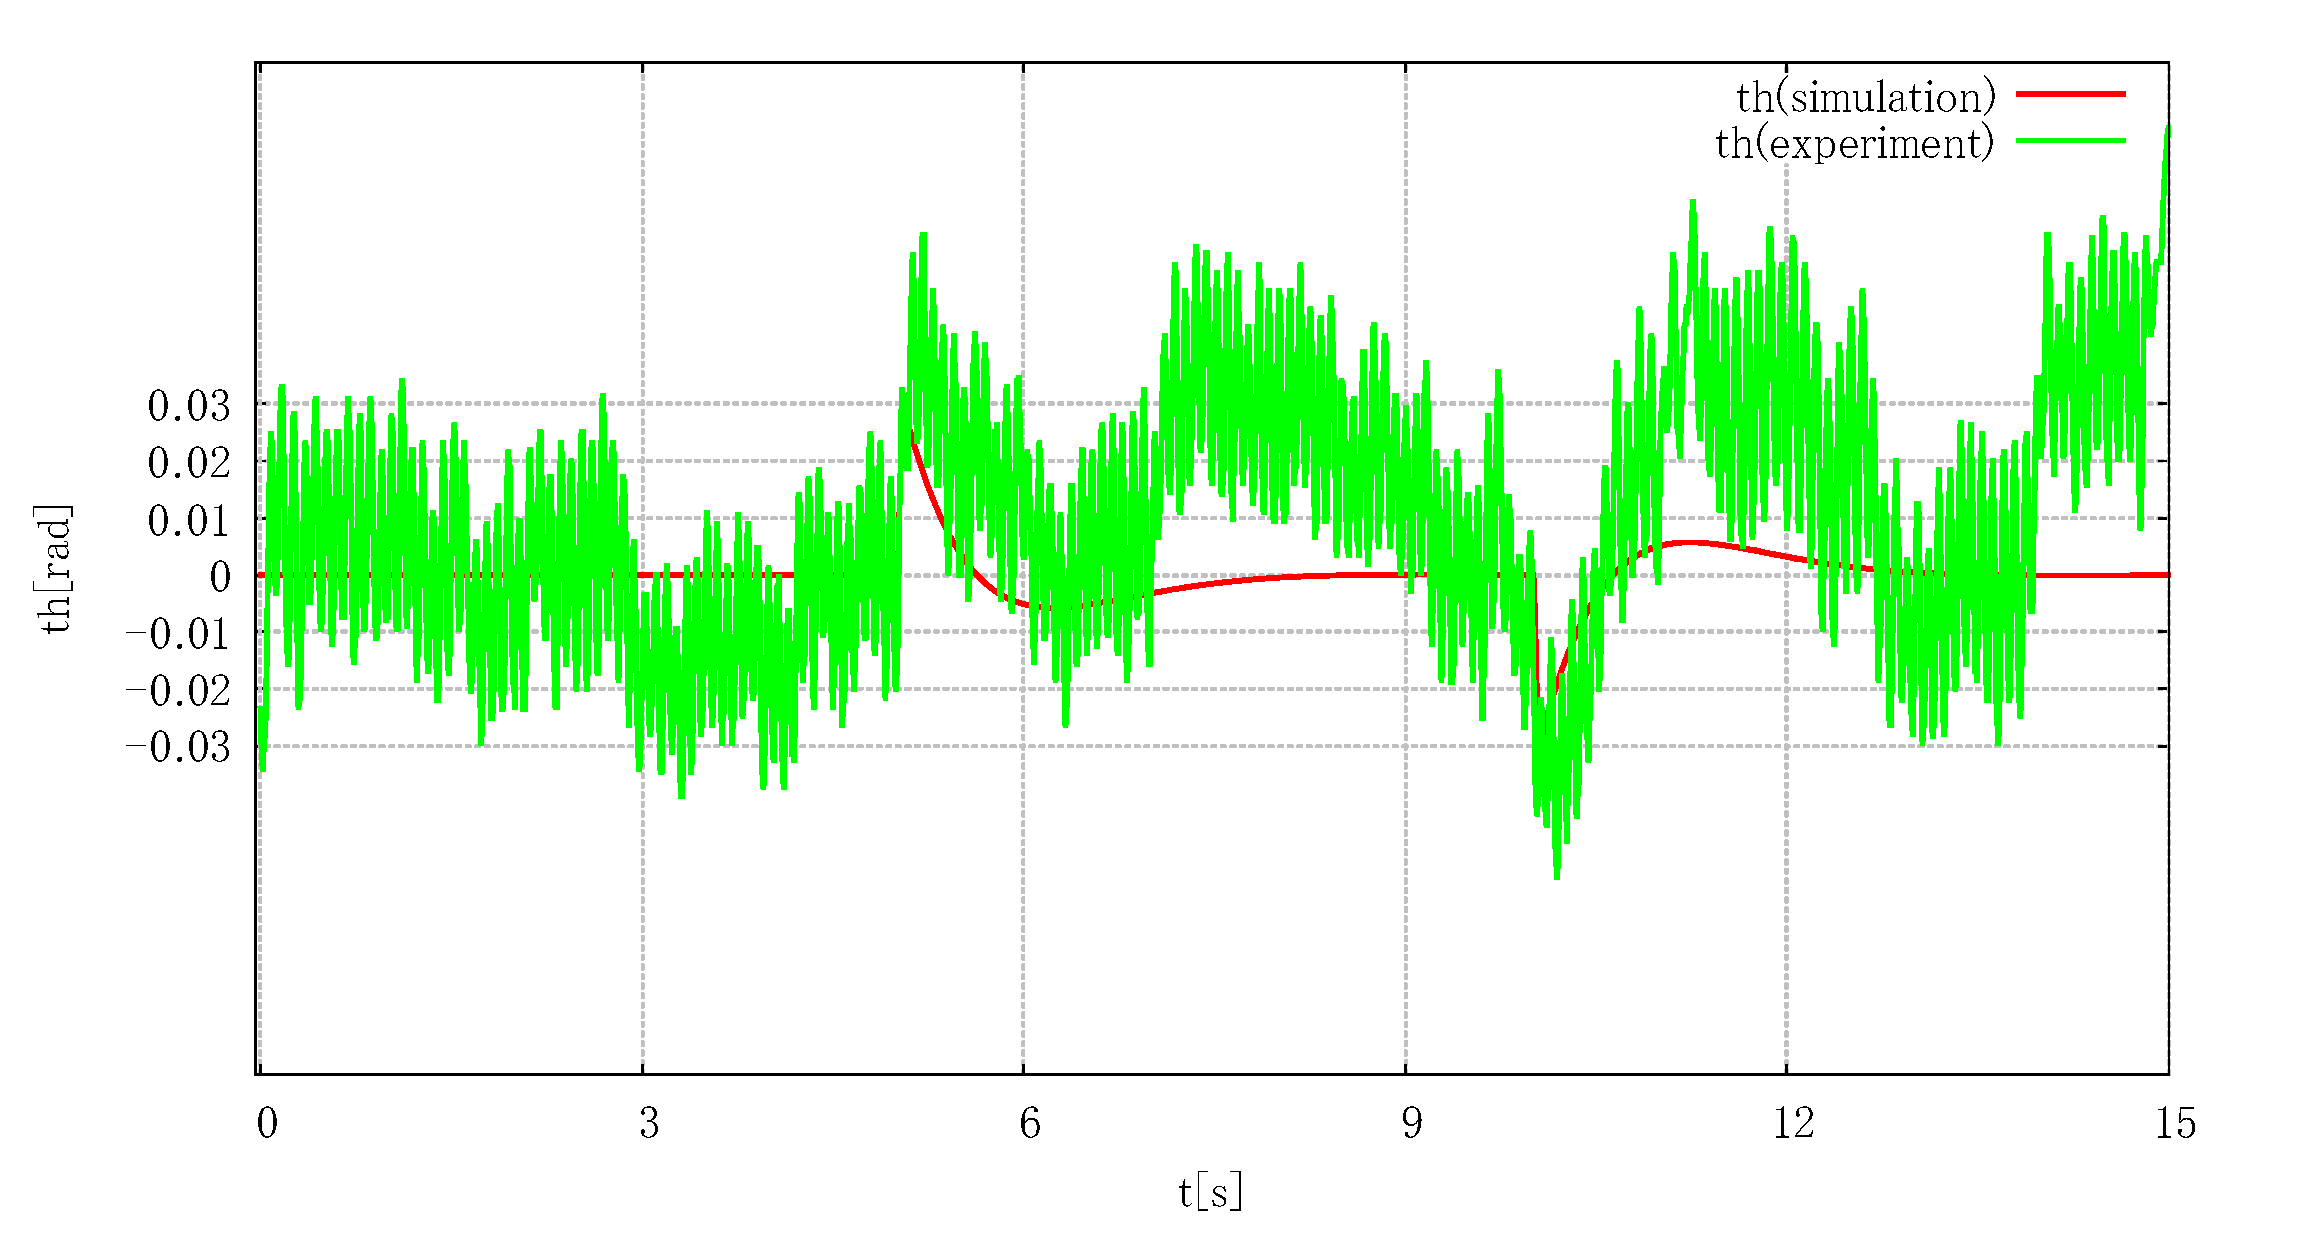
\includegraphics[width=0.4\linewidth]{gazo/experiment_Q56obs30dt05TH.eps}
		\caption{比較結果その2(左図がr,右図が$\theta$)}
		\label{image:sono2}
	\end{figure}
	\begin{figure}[H]
		\centering
		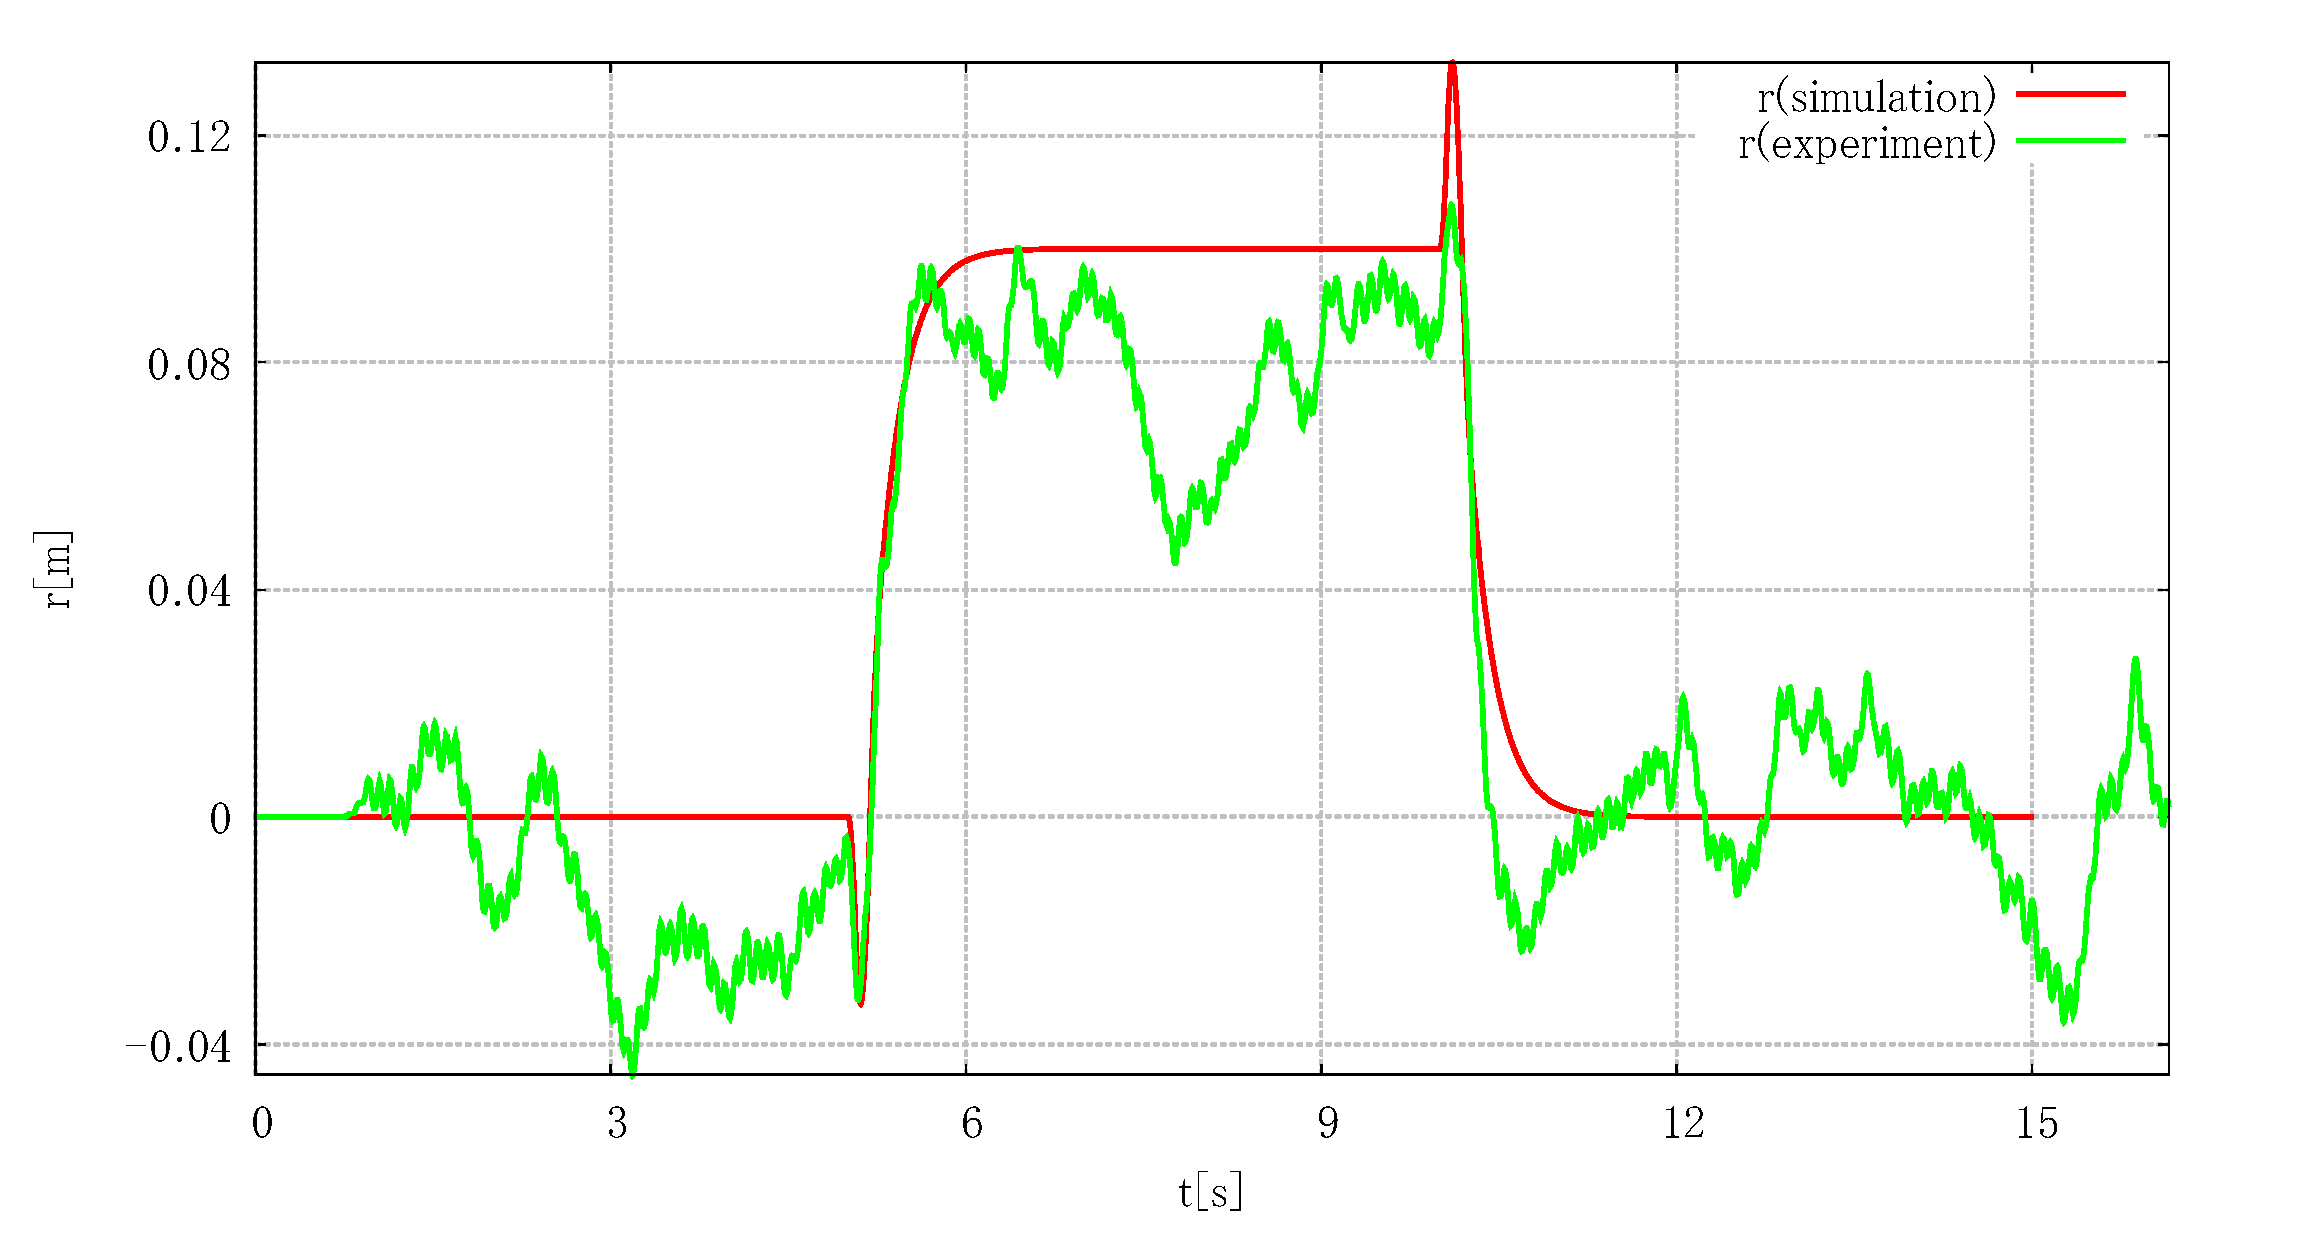
\includegraphics[width=0.4\linewidth]{gazo/experiment_Q65obs30dt05R.eps}
		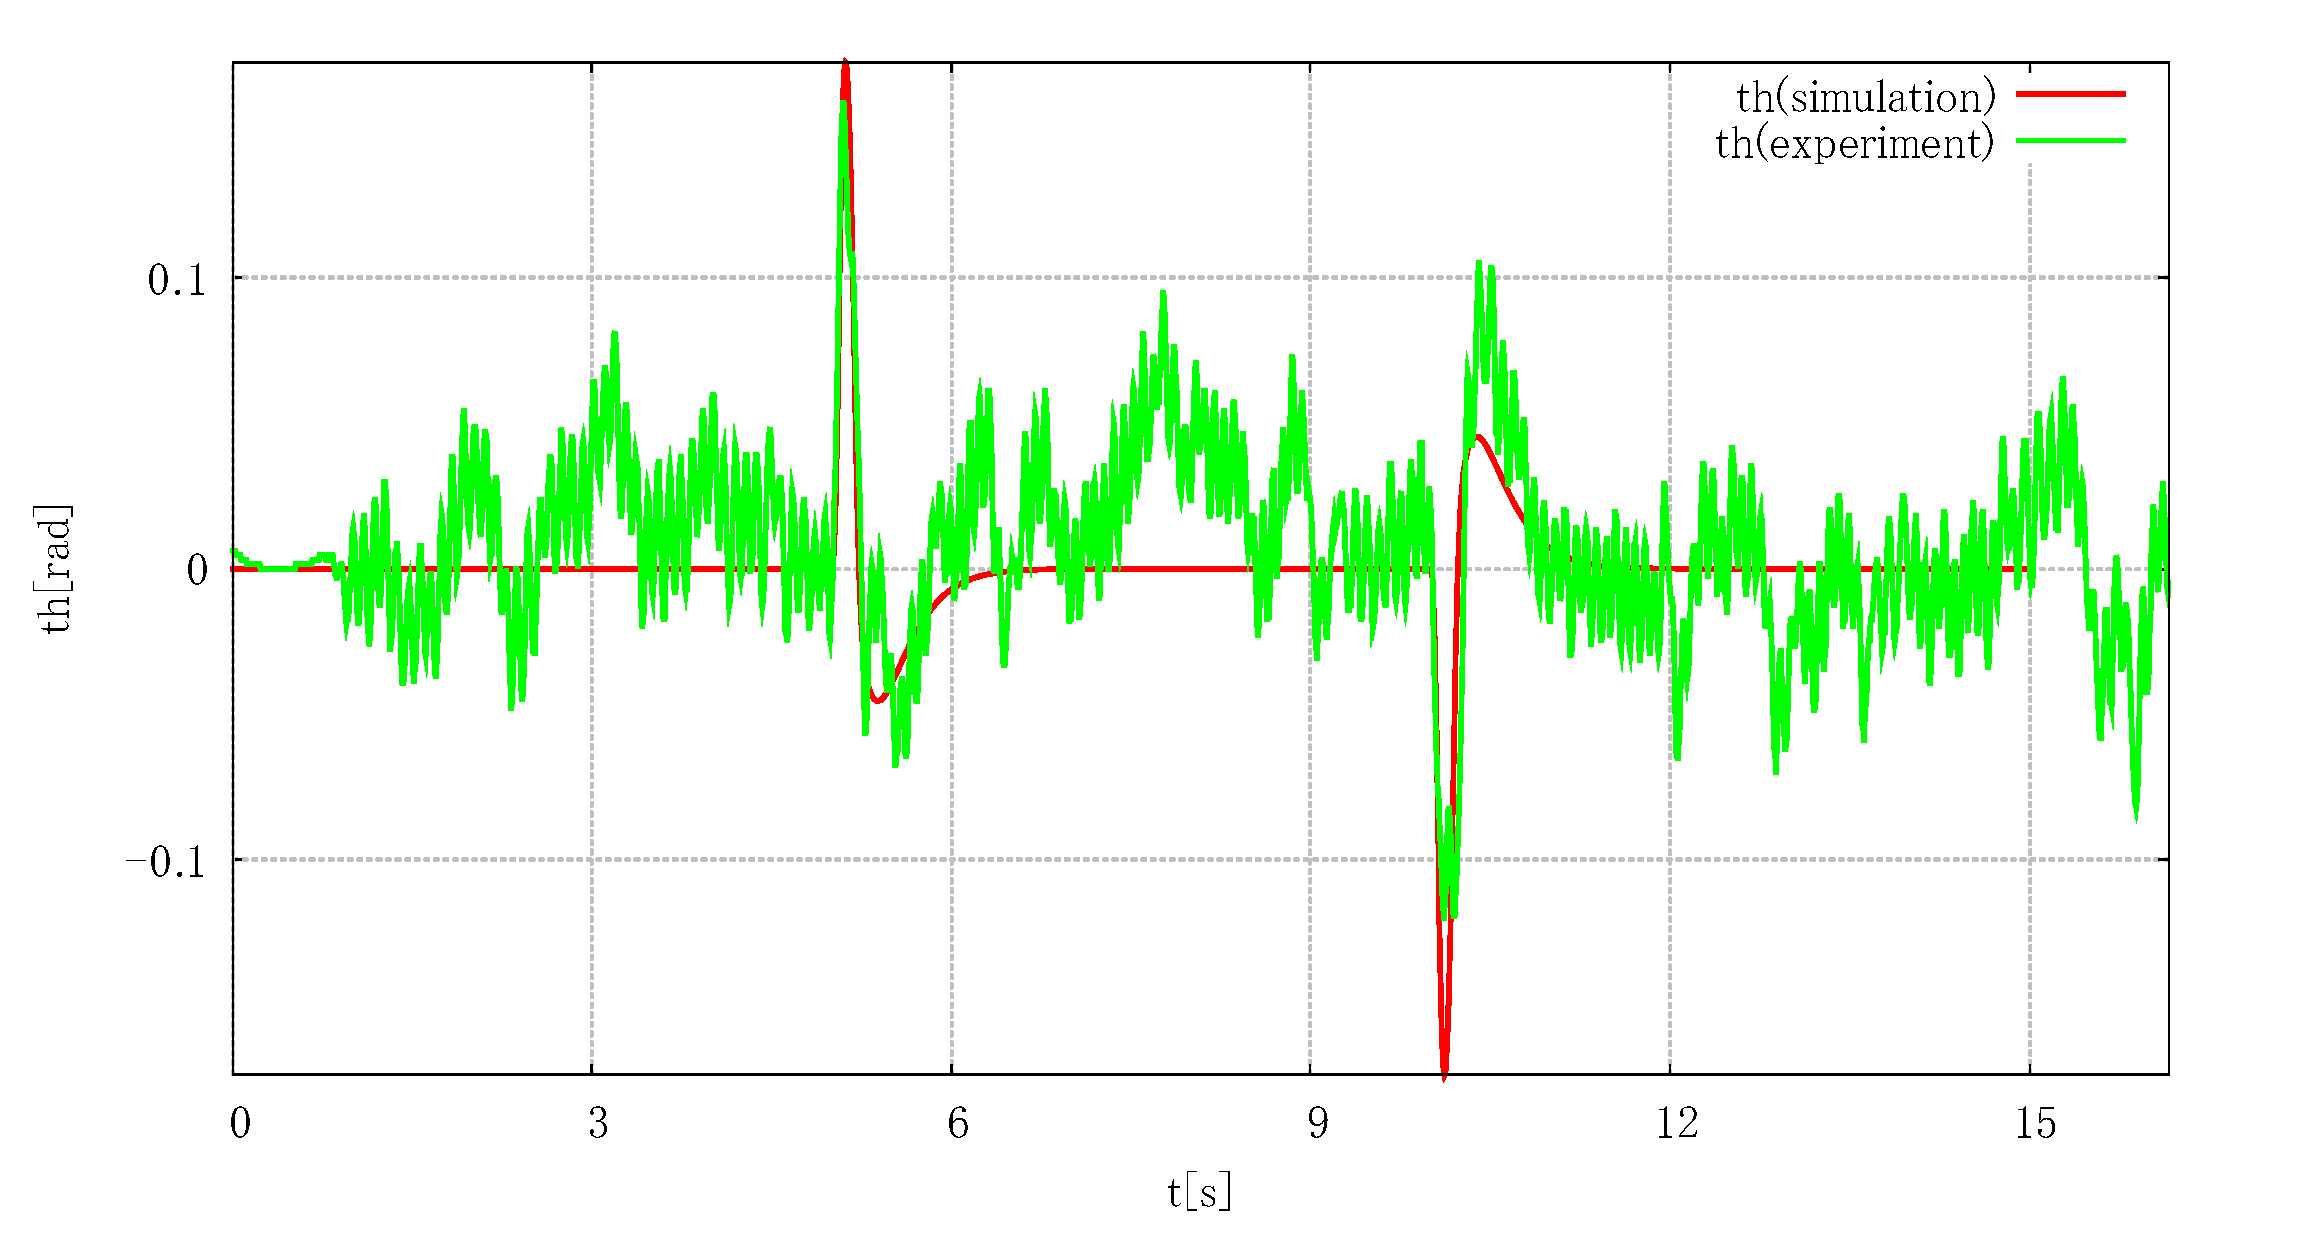
\includegraphics[width=0.4\linewidth]{gazo/experiment_Q65obs30dt05TH.eps}
		\caption{比較結果その3(左図がr,右図が$\theta$)}
		\label{image:sono3}
	\end{figure}
	\begin{figure}[H]
		\centering
		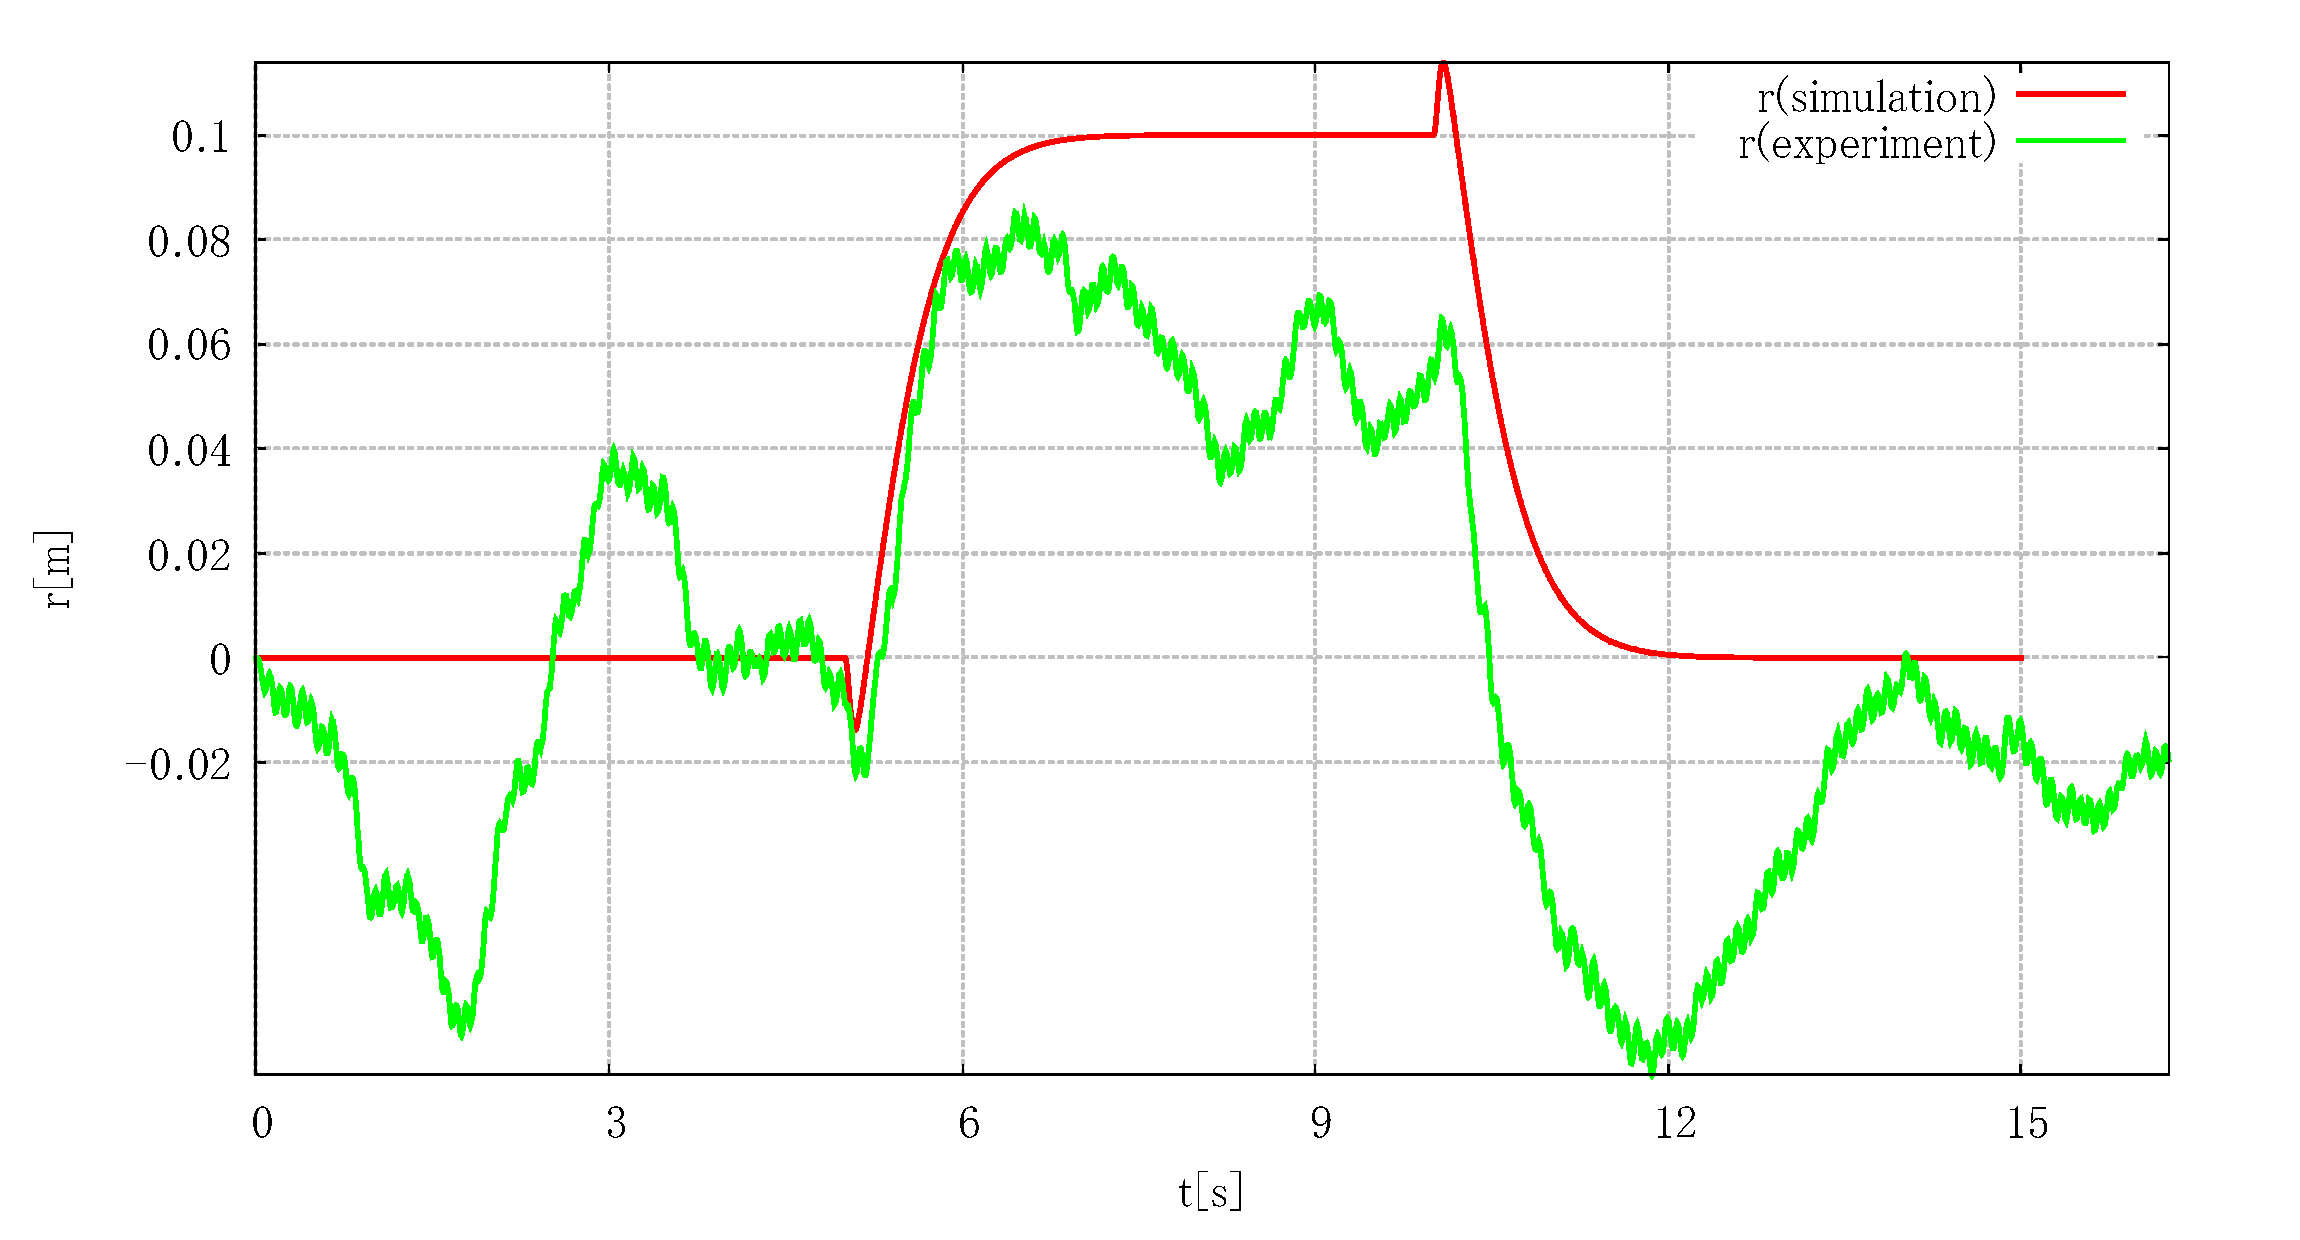
\includegraphics[width=0.4\linewidth]{gazo/experiment_Q55obs60dt05R.eps}
		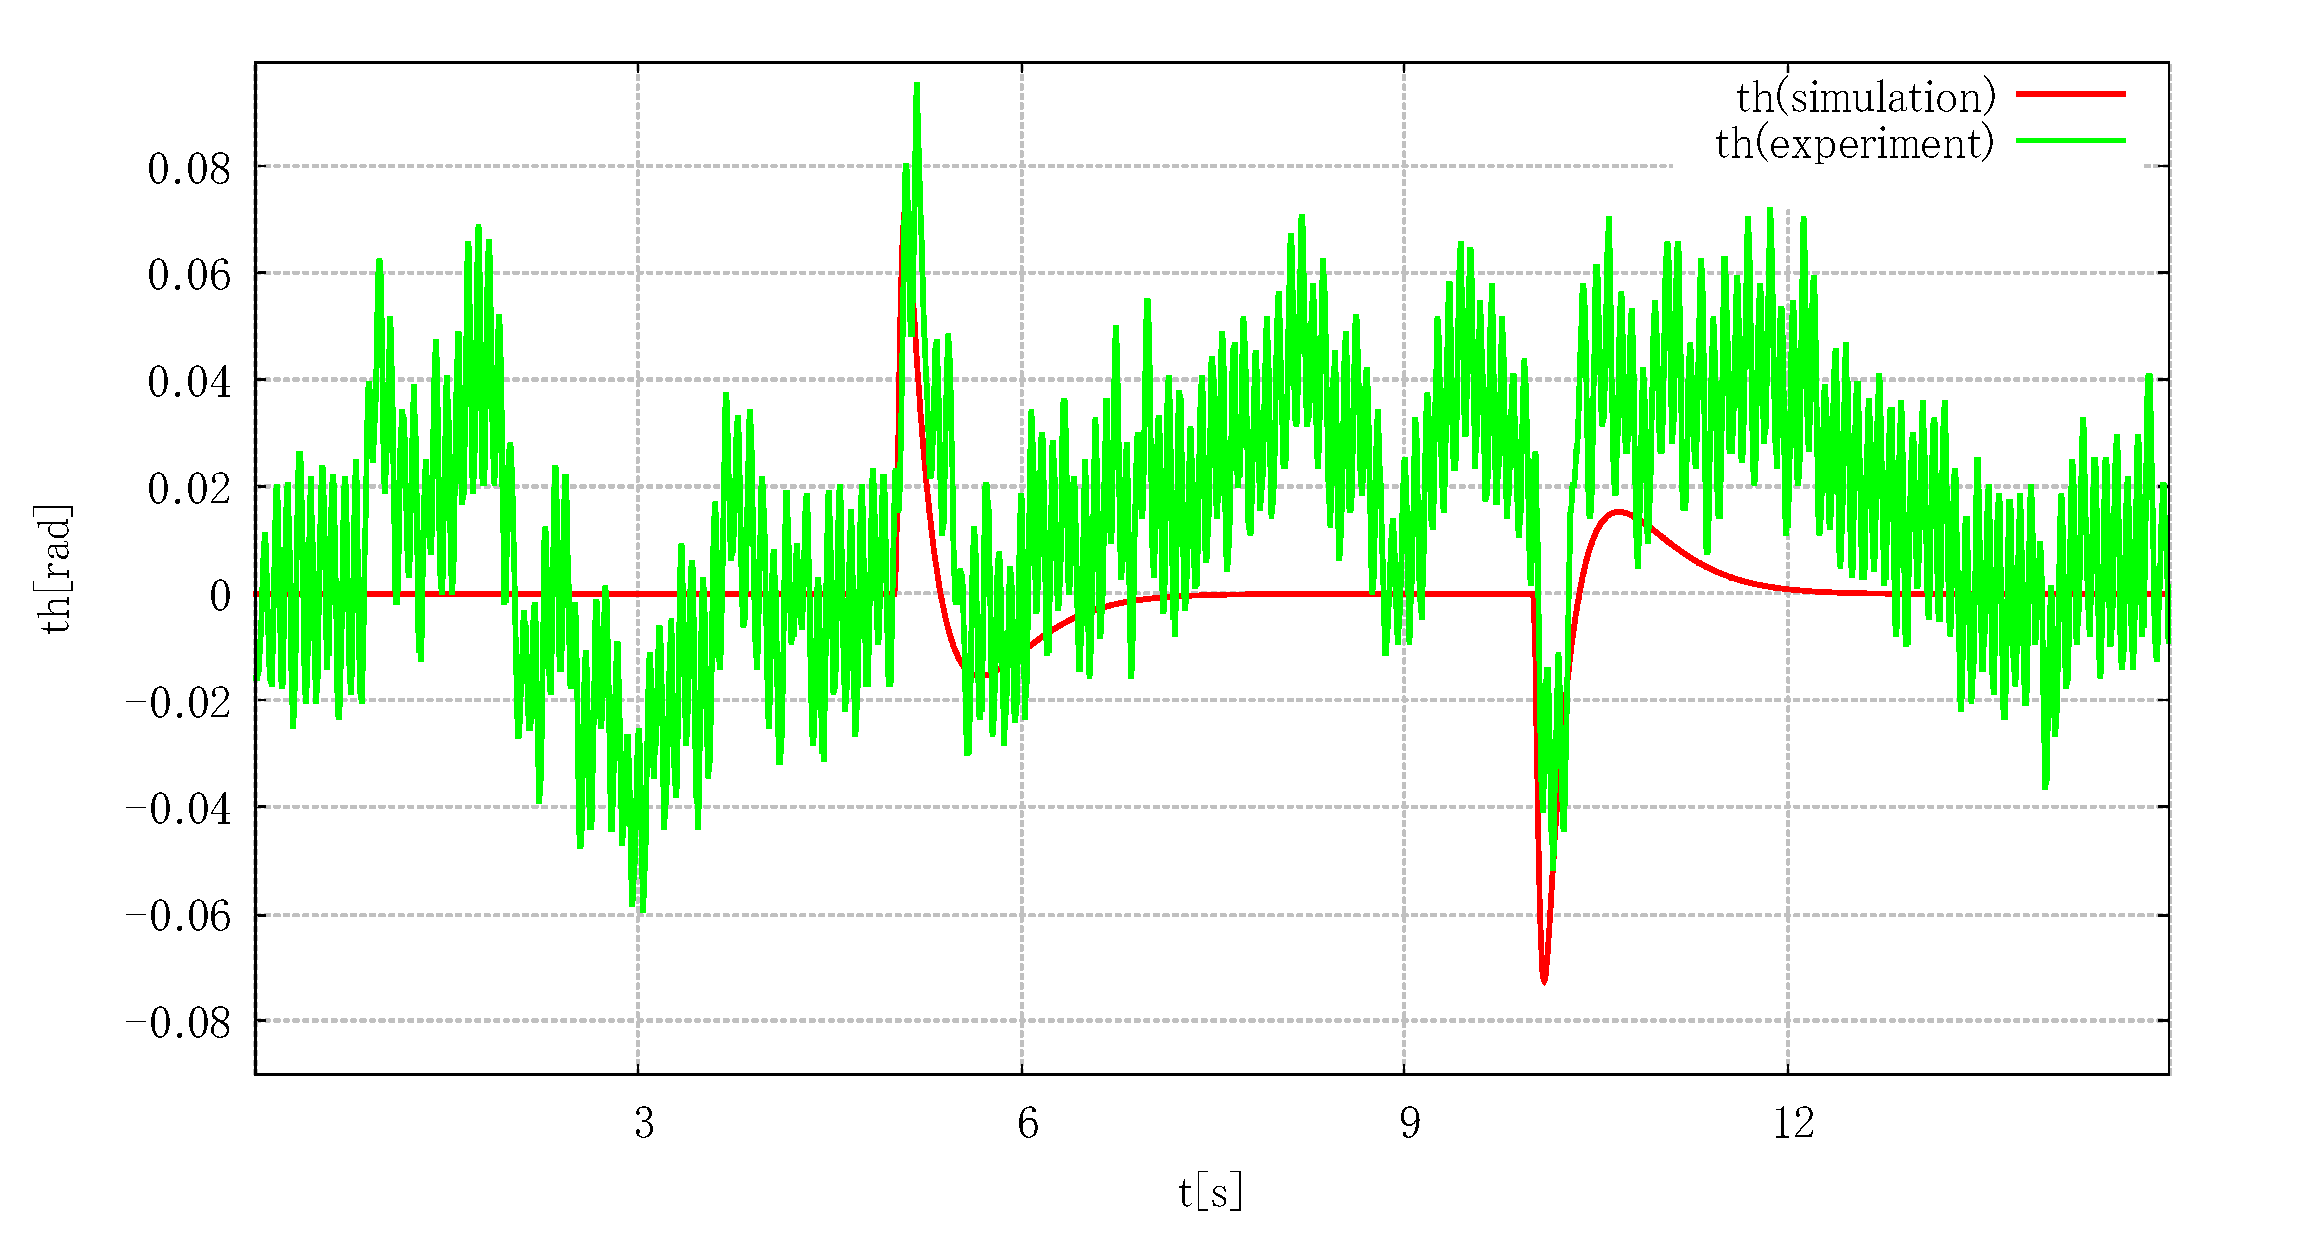
\includegraphics[width=0.4\linewidth]{gazo/experiment_Q55obs60dt05TH.eps}
		\caption{比較結果その4(左図がr,右図が$\theta$)}
		\label{image:sono4}
	\end{figure}
	\begin{figure}[H]
		\centering
		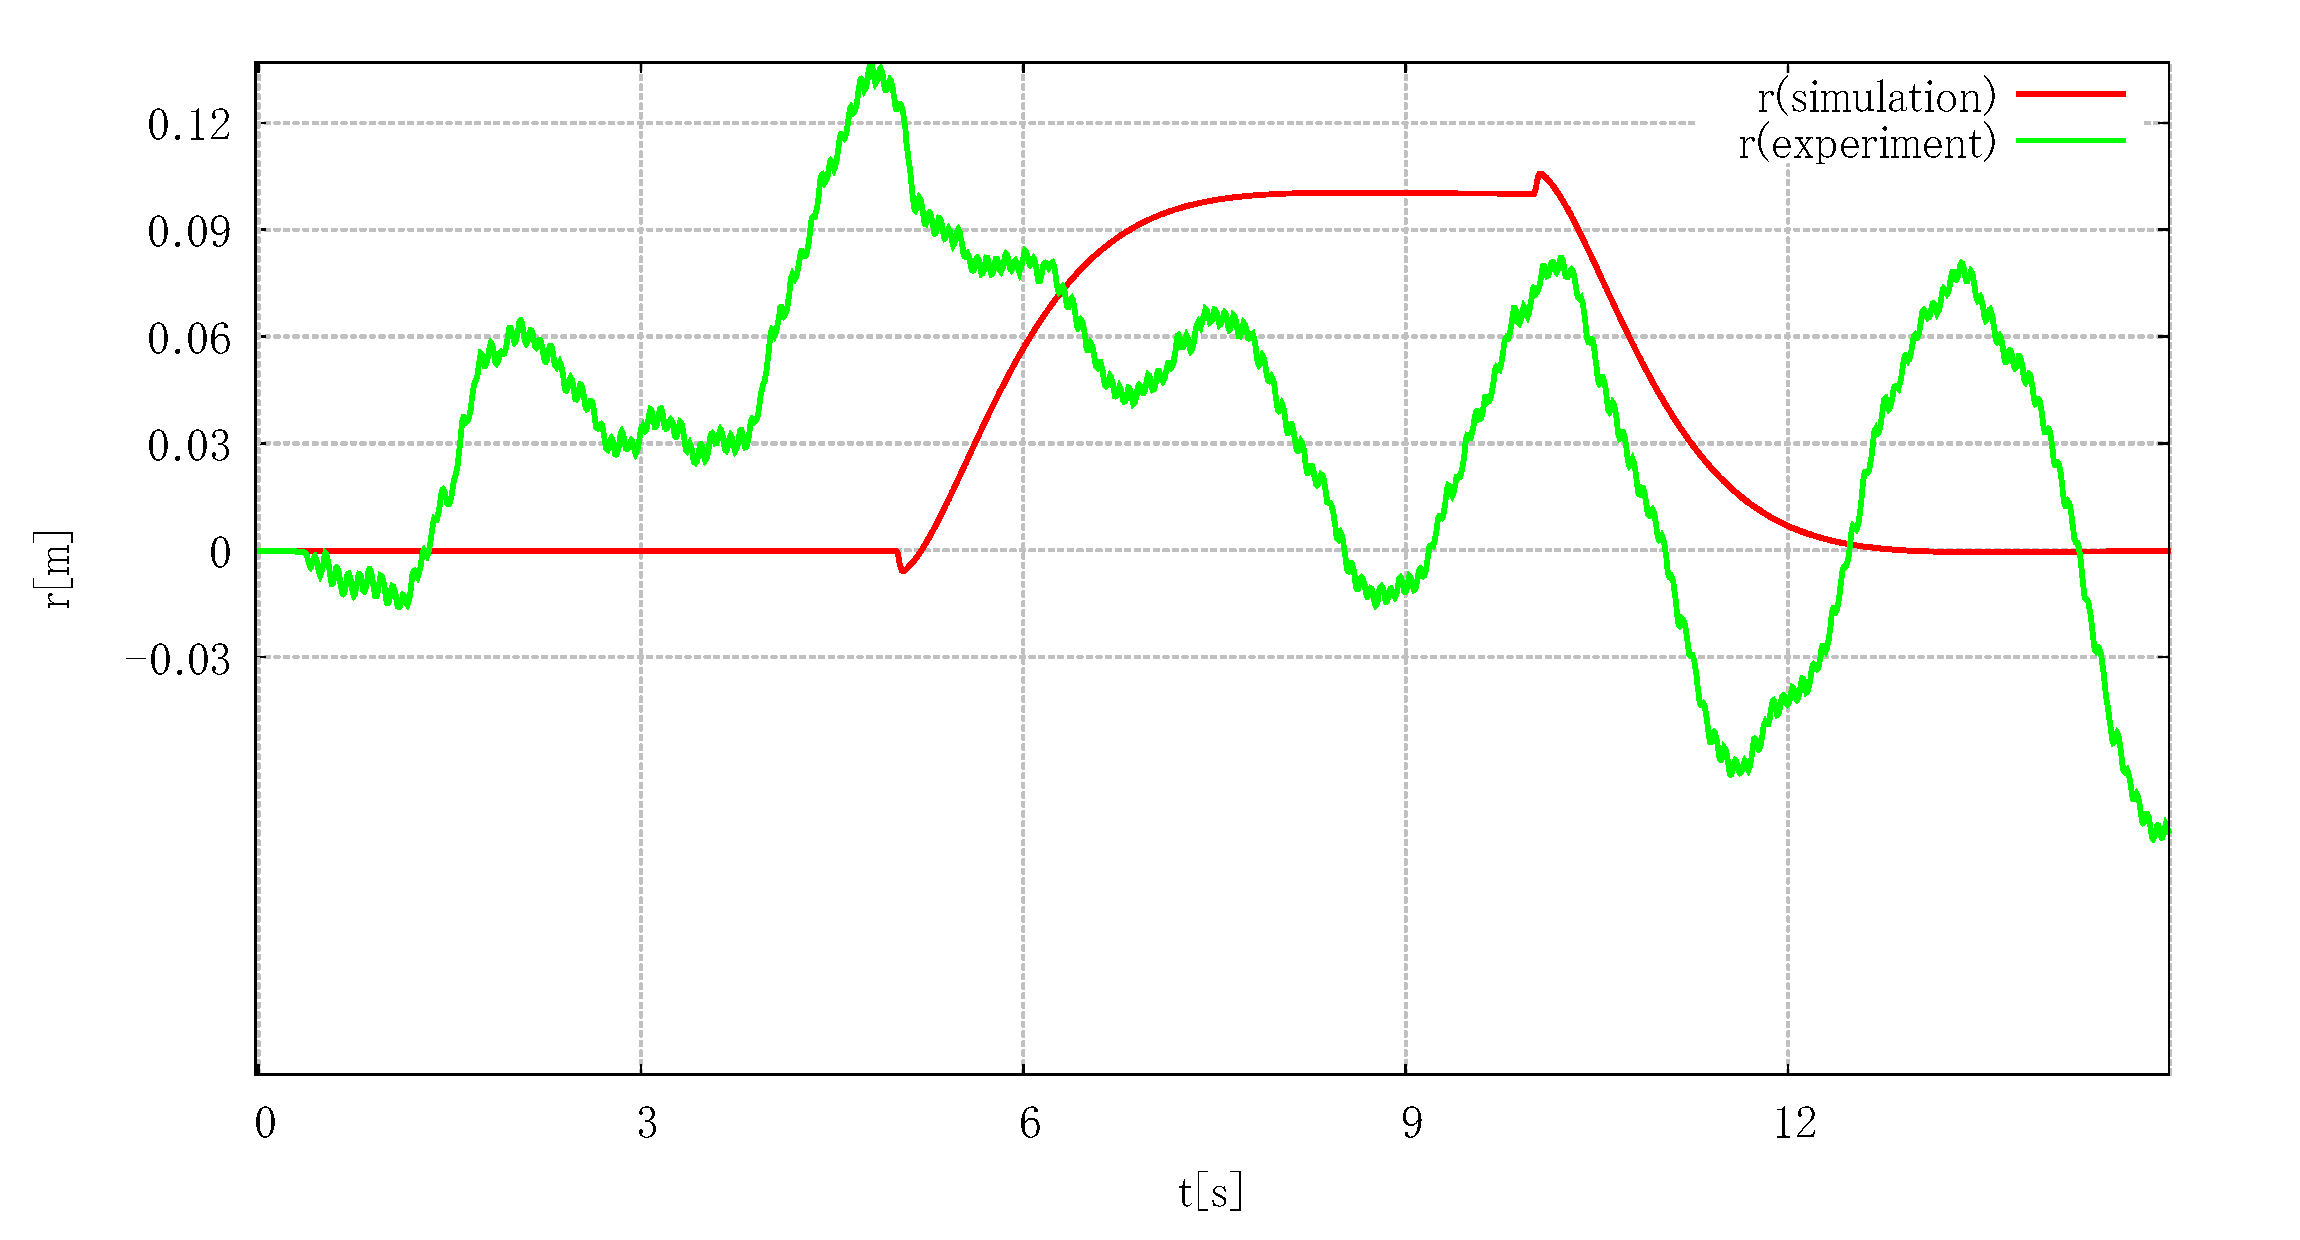
\includegraphics[width=0.4\linewidth]{gazo/experiment_Q56obs60dt05R.eps}
		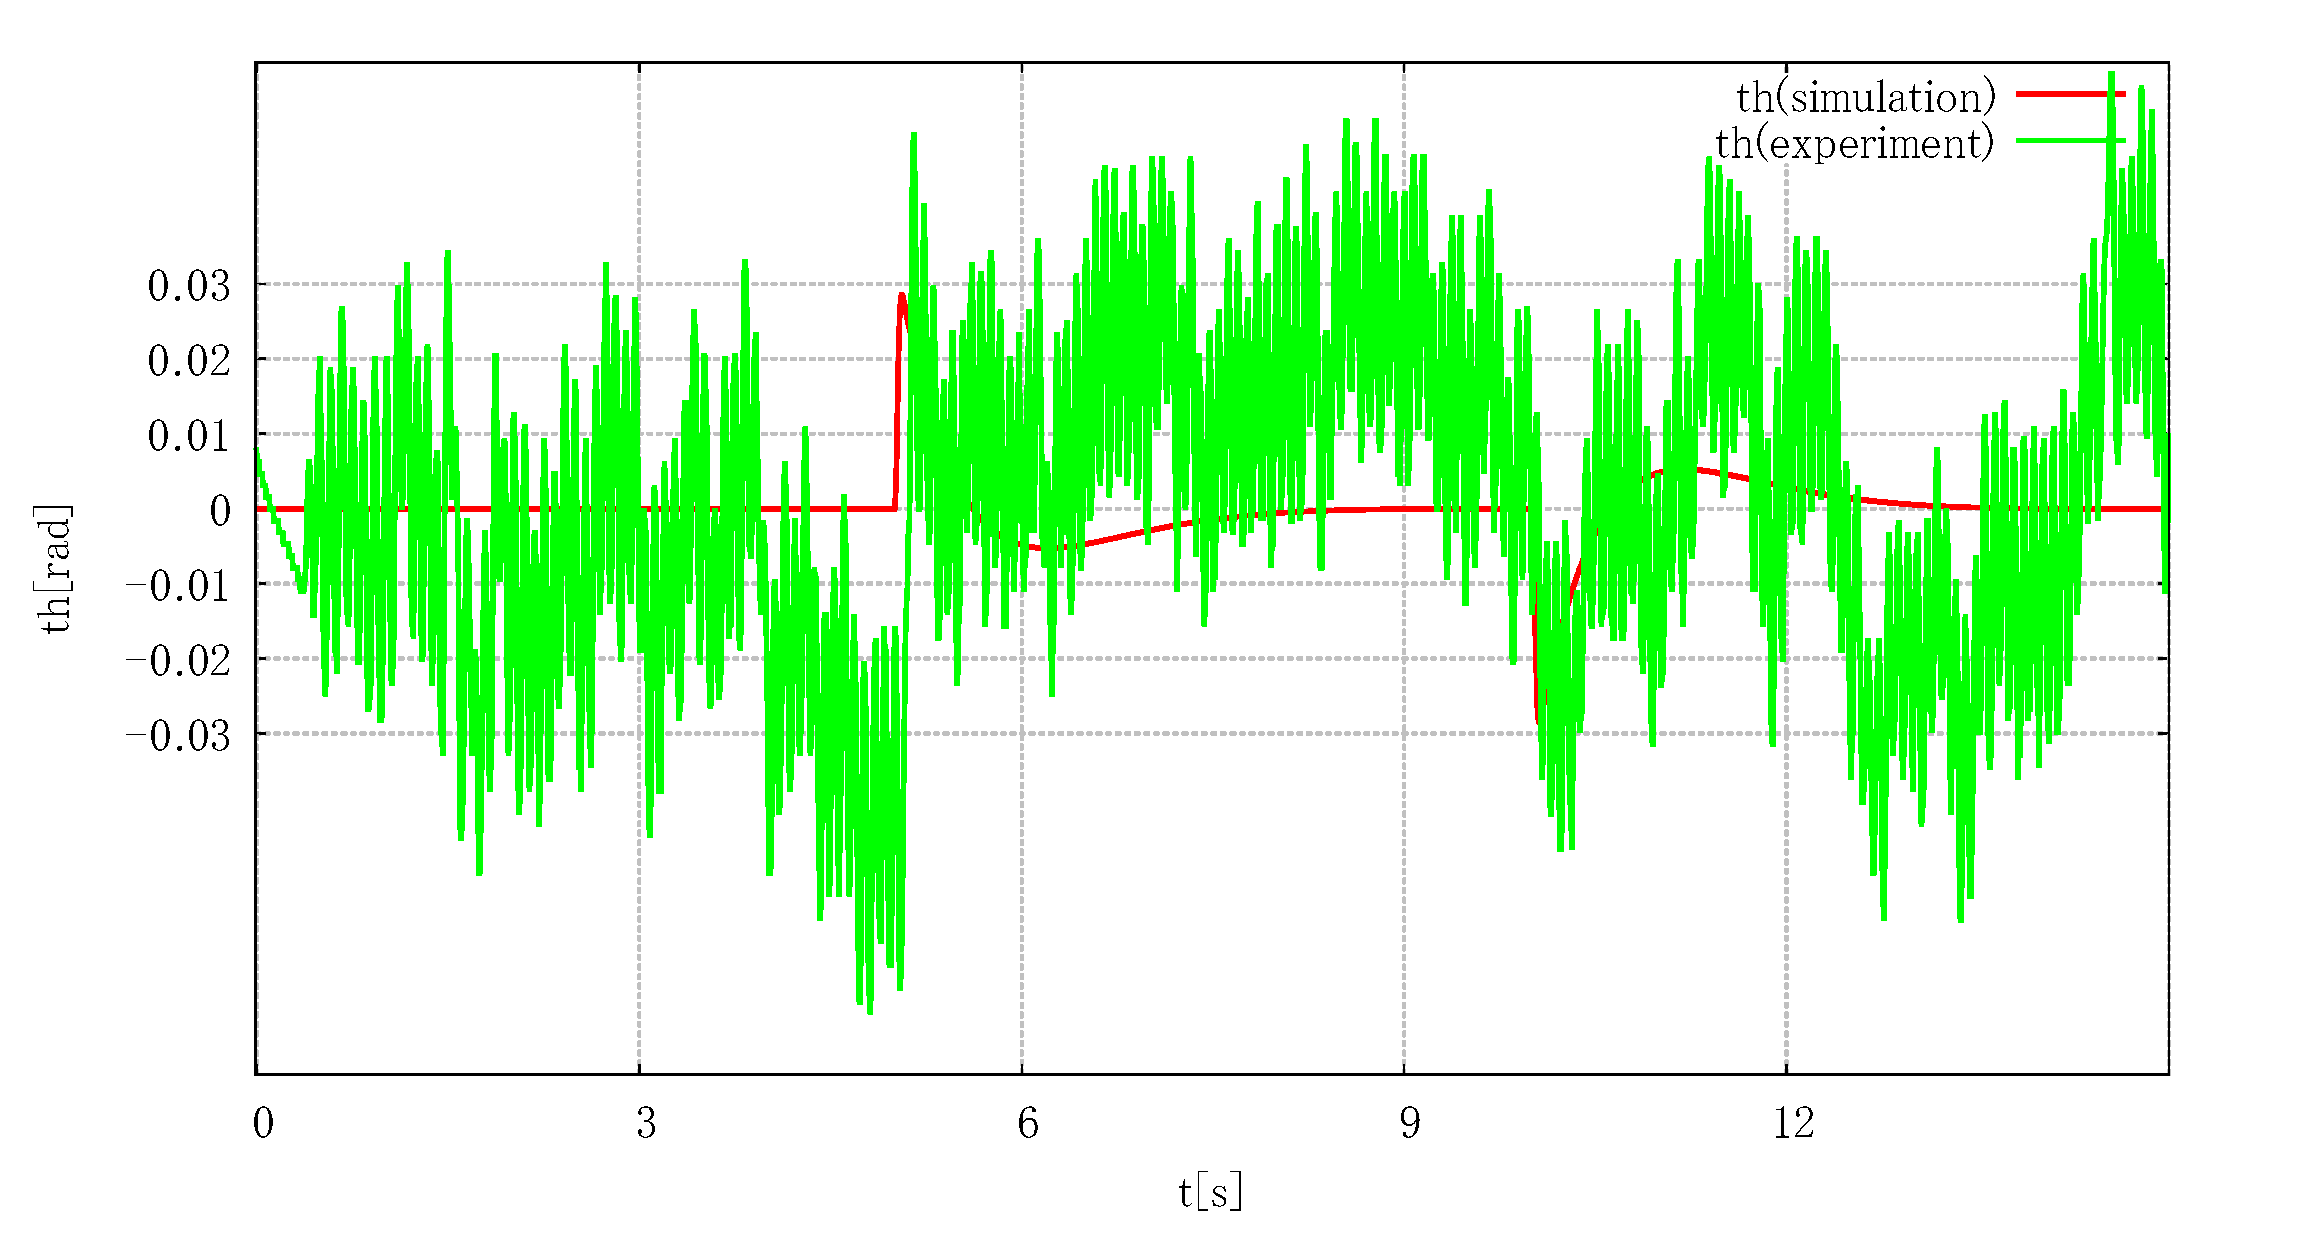
\includegraphics[width=0.4\linewidth]{gazo/experiment_Q56obs60dt05TH.eps}
		\caption{比較結果その5(左図がr,右図が$\theta$)}
		\label{image:sono5}
	\end{figure}
	\begin{figure}[H]
		\centering
		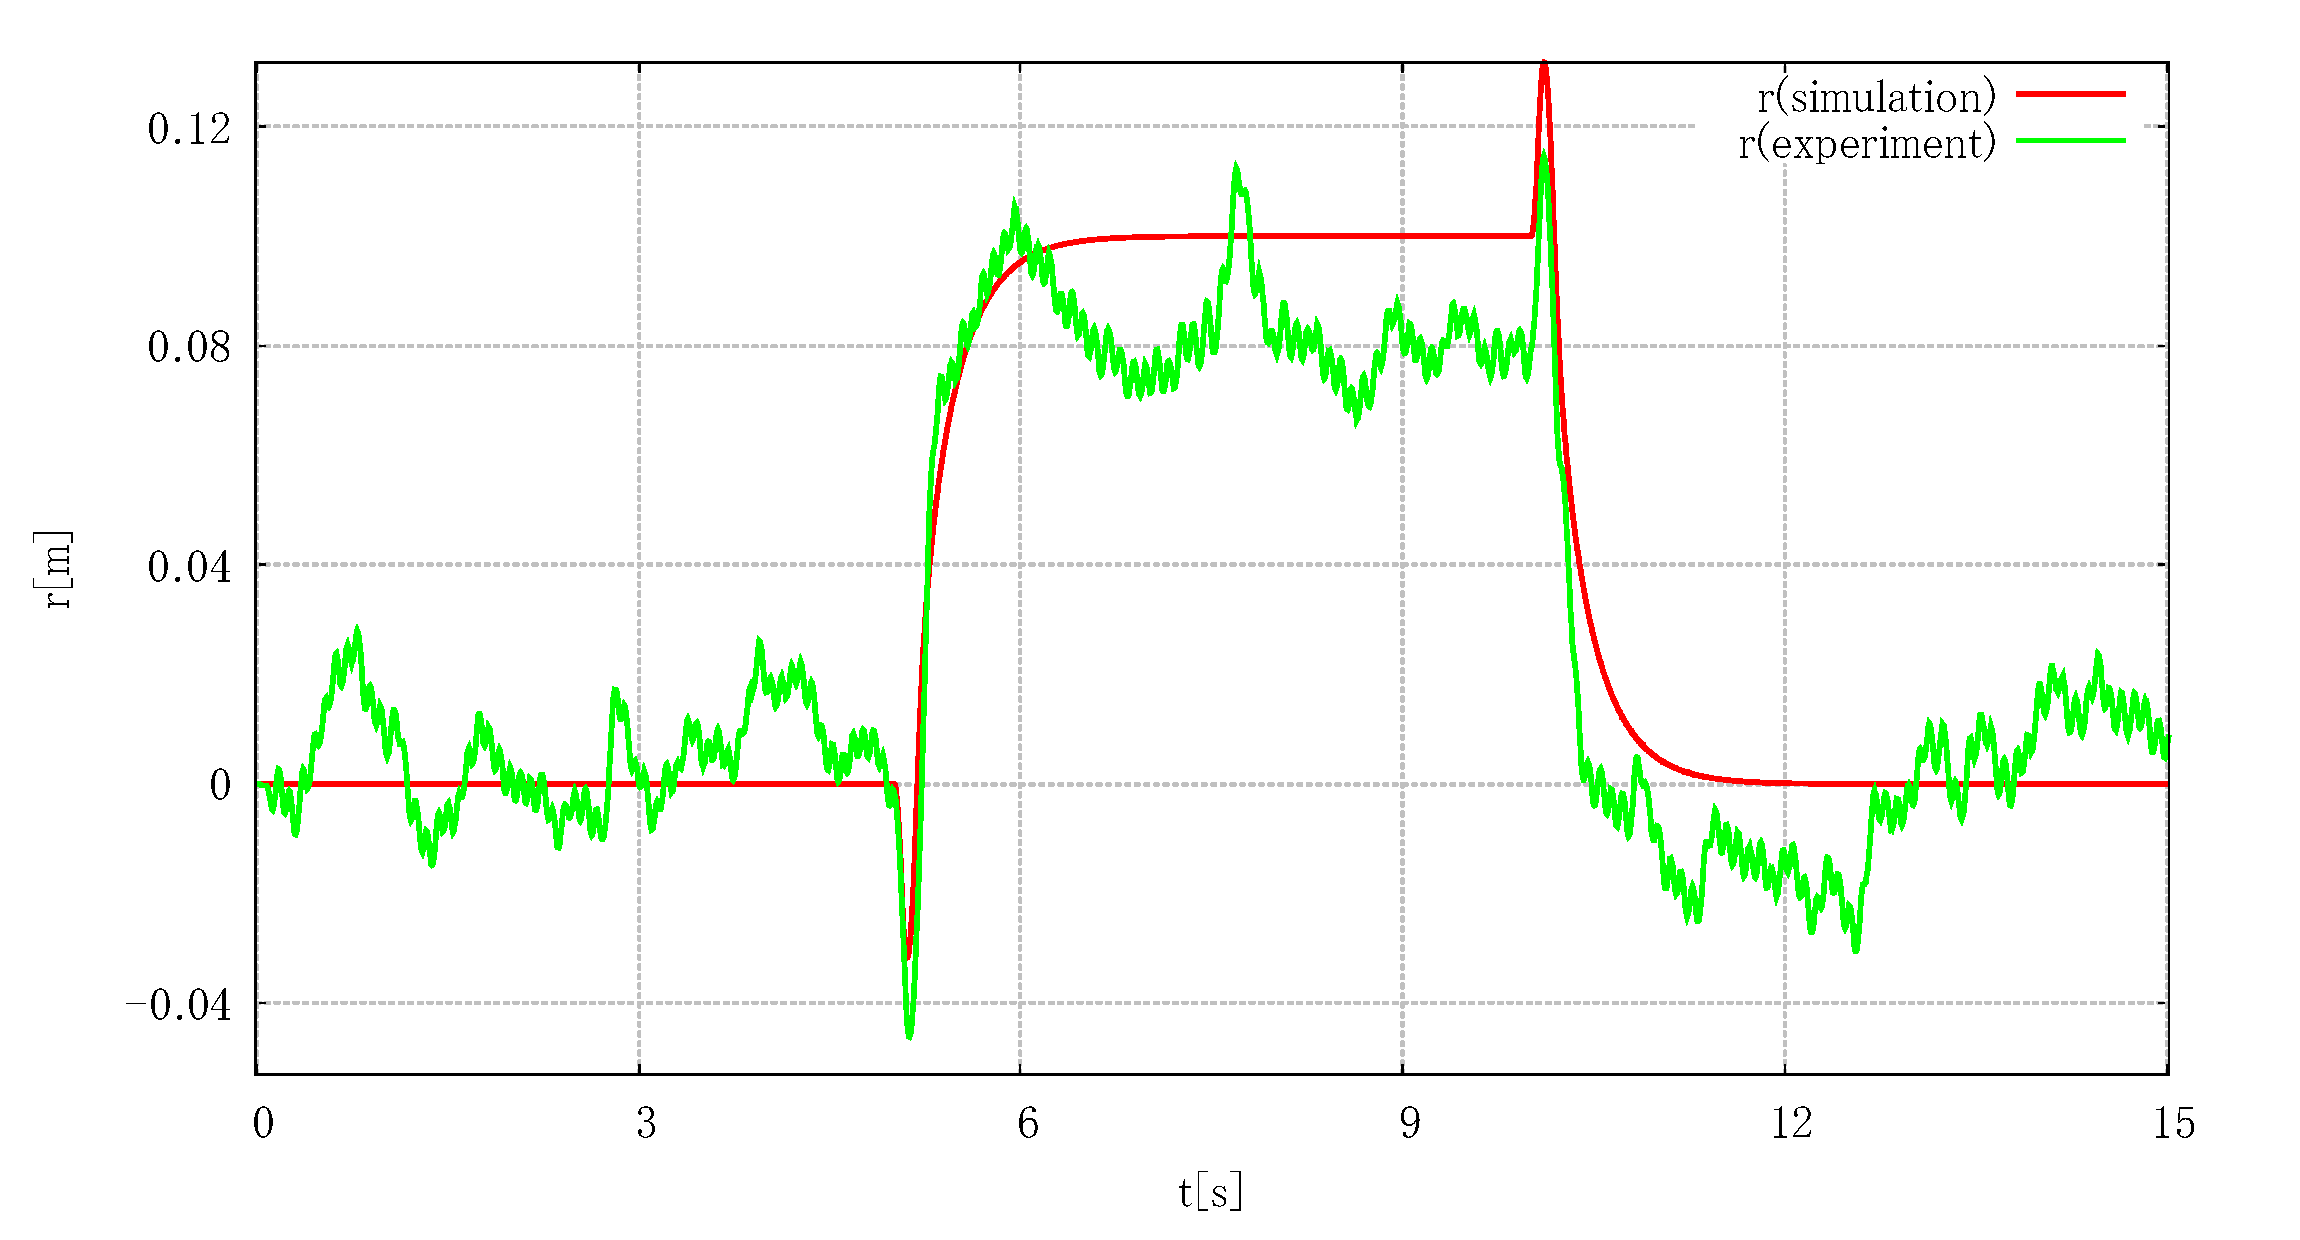
\includegraphics[width=0.4\linewidth]{gazo/experiment_Q65obs60dt05R.eps}
		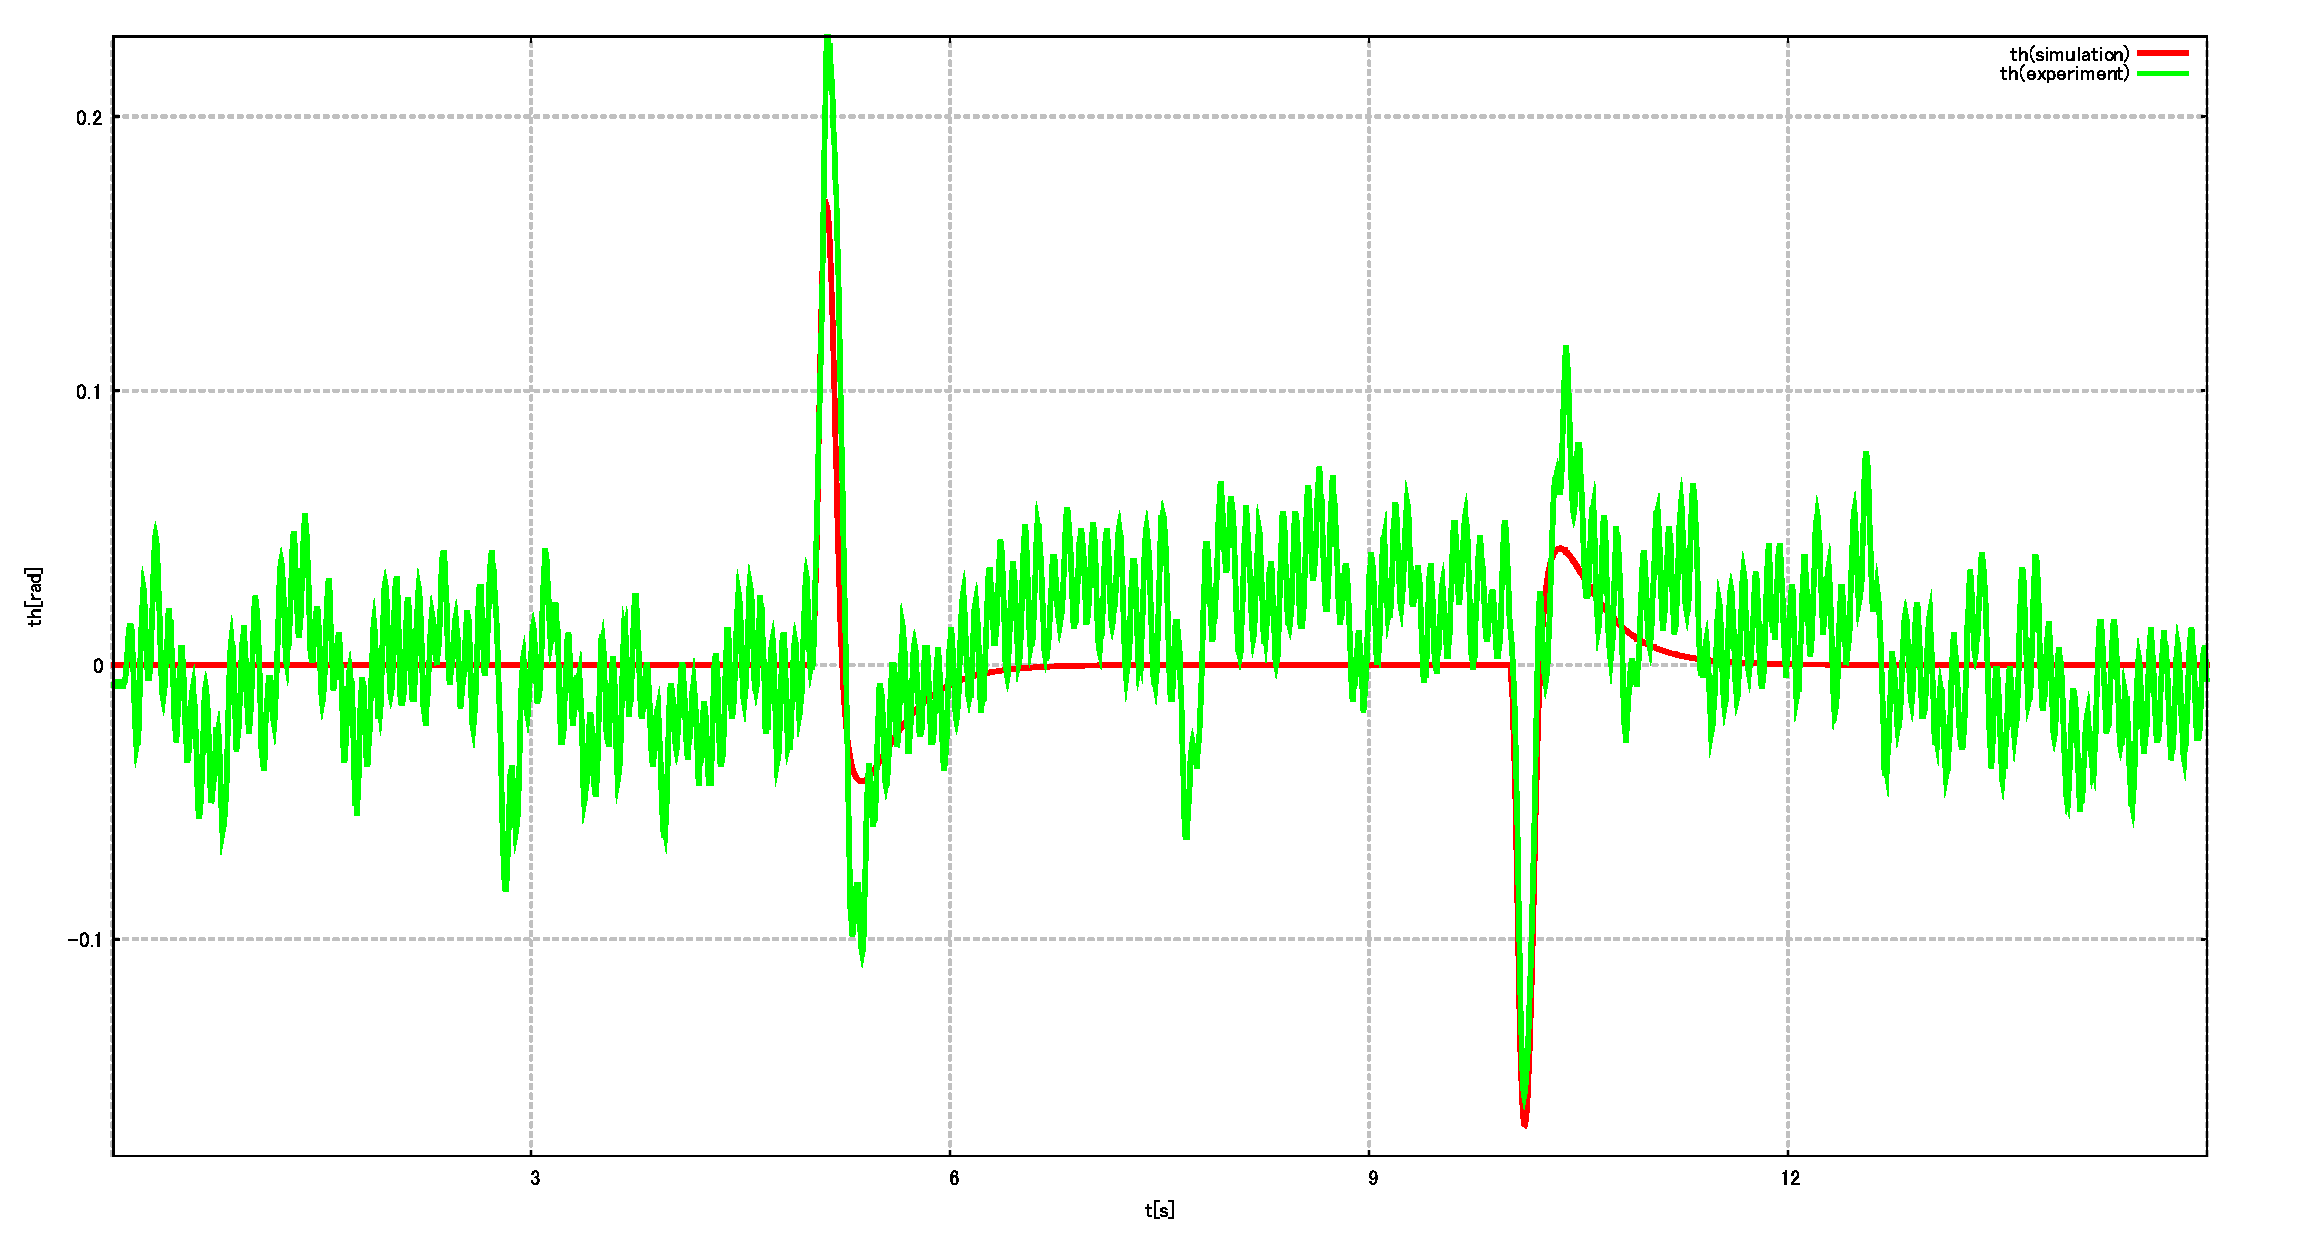
\includegraphics[width=0.4\linewidth]{gazo/experiment_Q65obs60dt05TH.eps}
		\caption{比較結果その6(左図がr,右図が$\theta$)}
		\label{image:sono6}
	\end{figure}
	\begin{figure}[H]
		\centering
		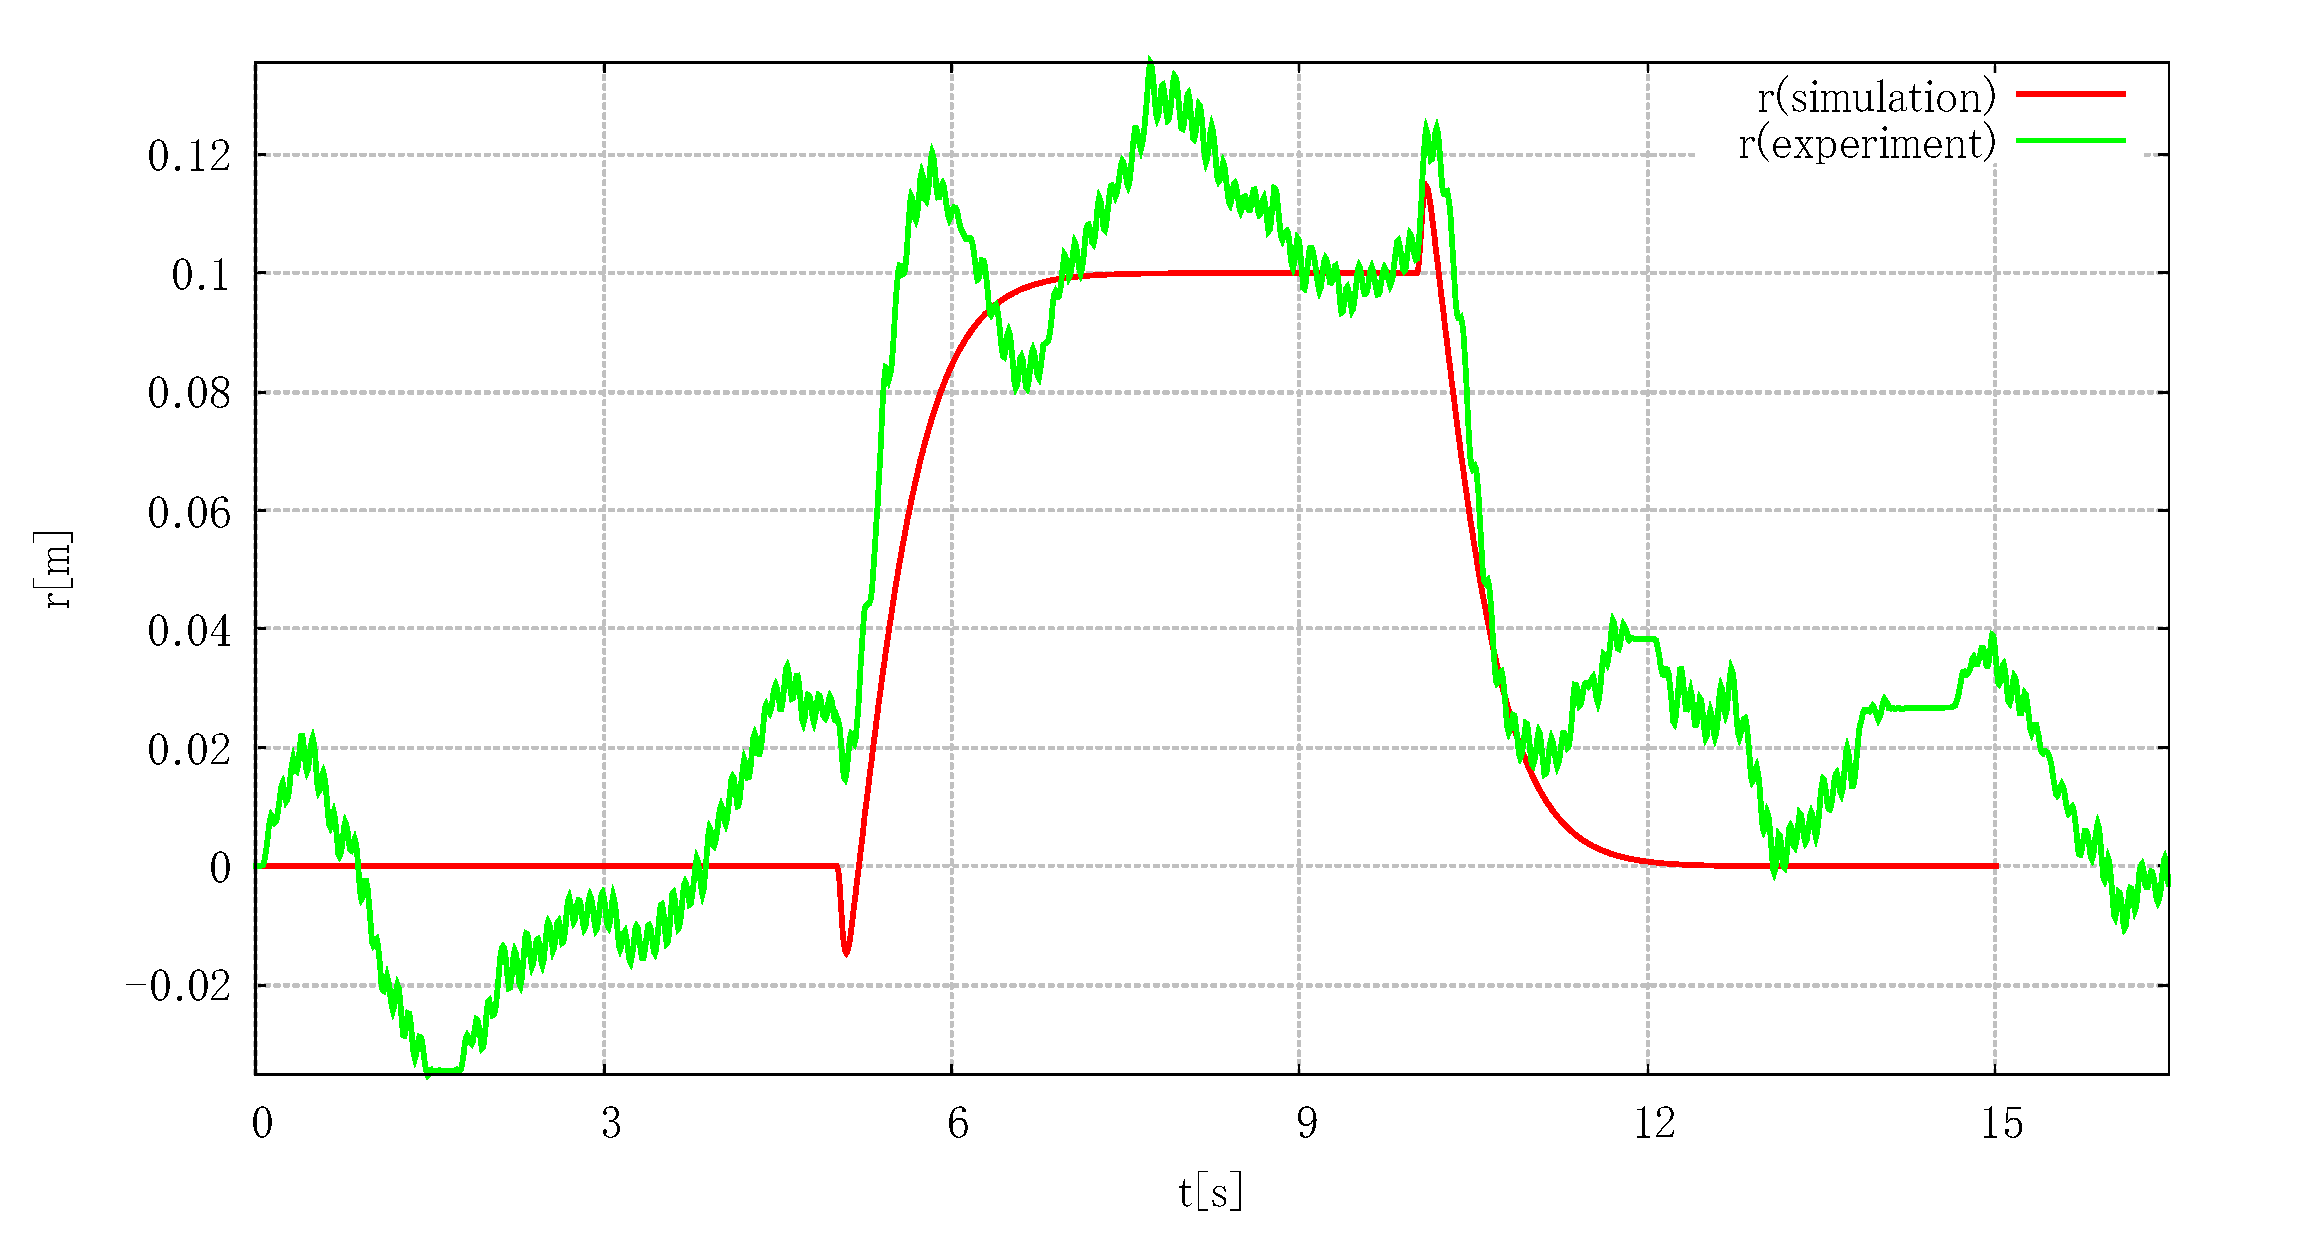
\includegraphics[width=0.4\linewidth]{gazo/experiment_Q55obs30dt10R.eps}
		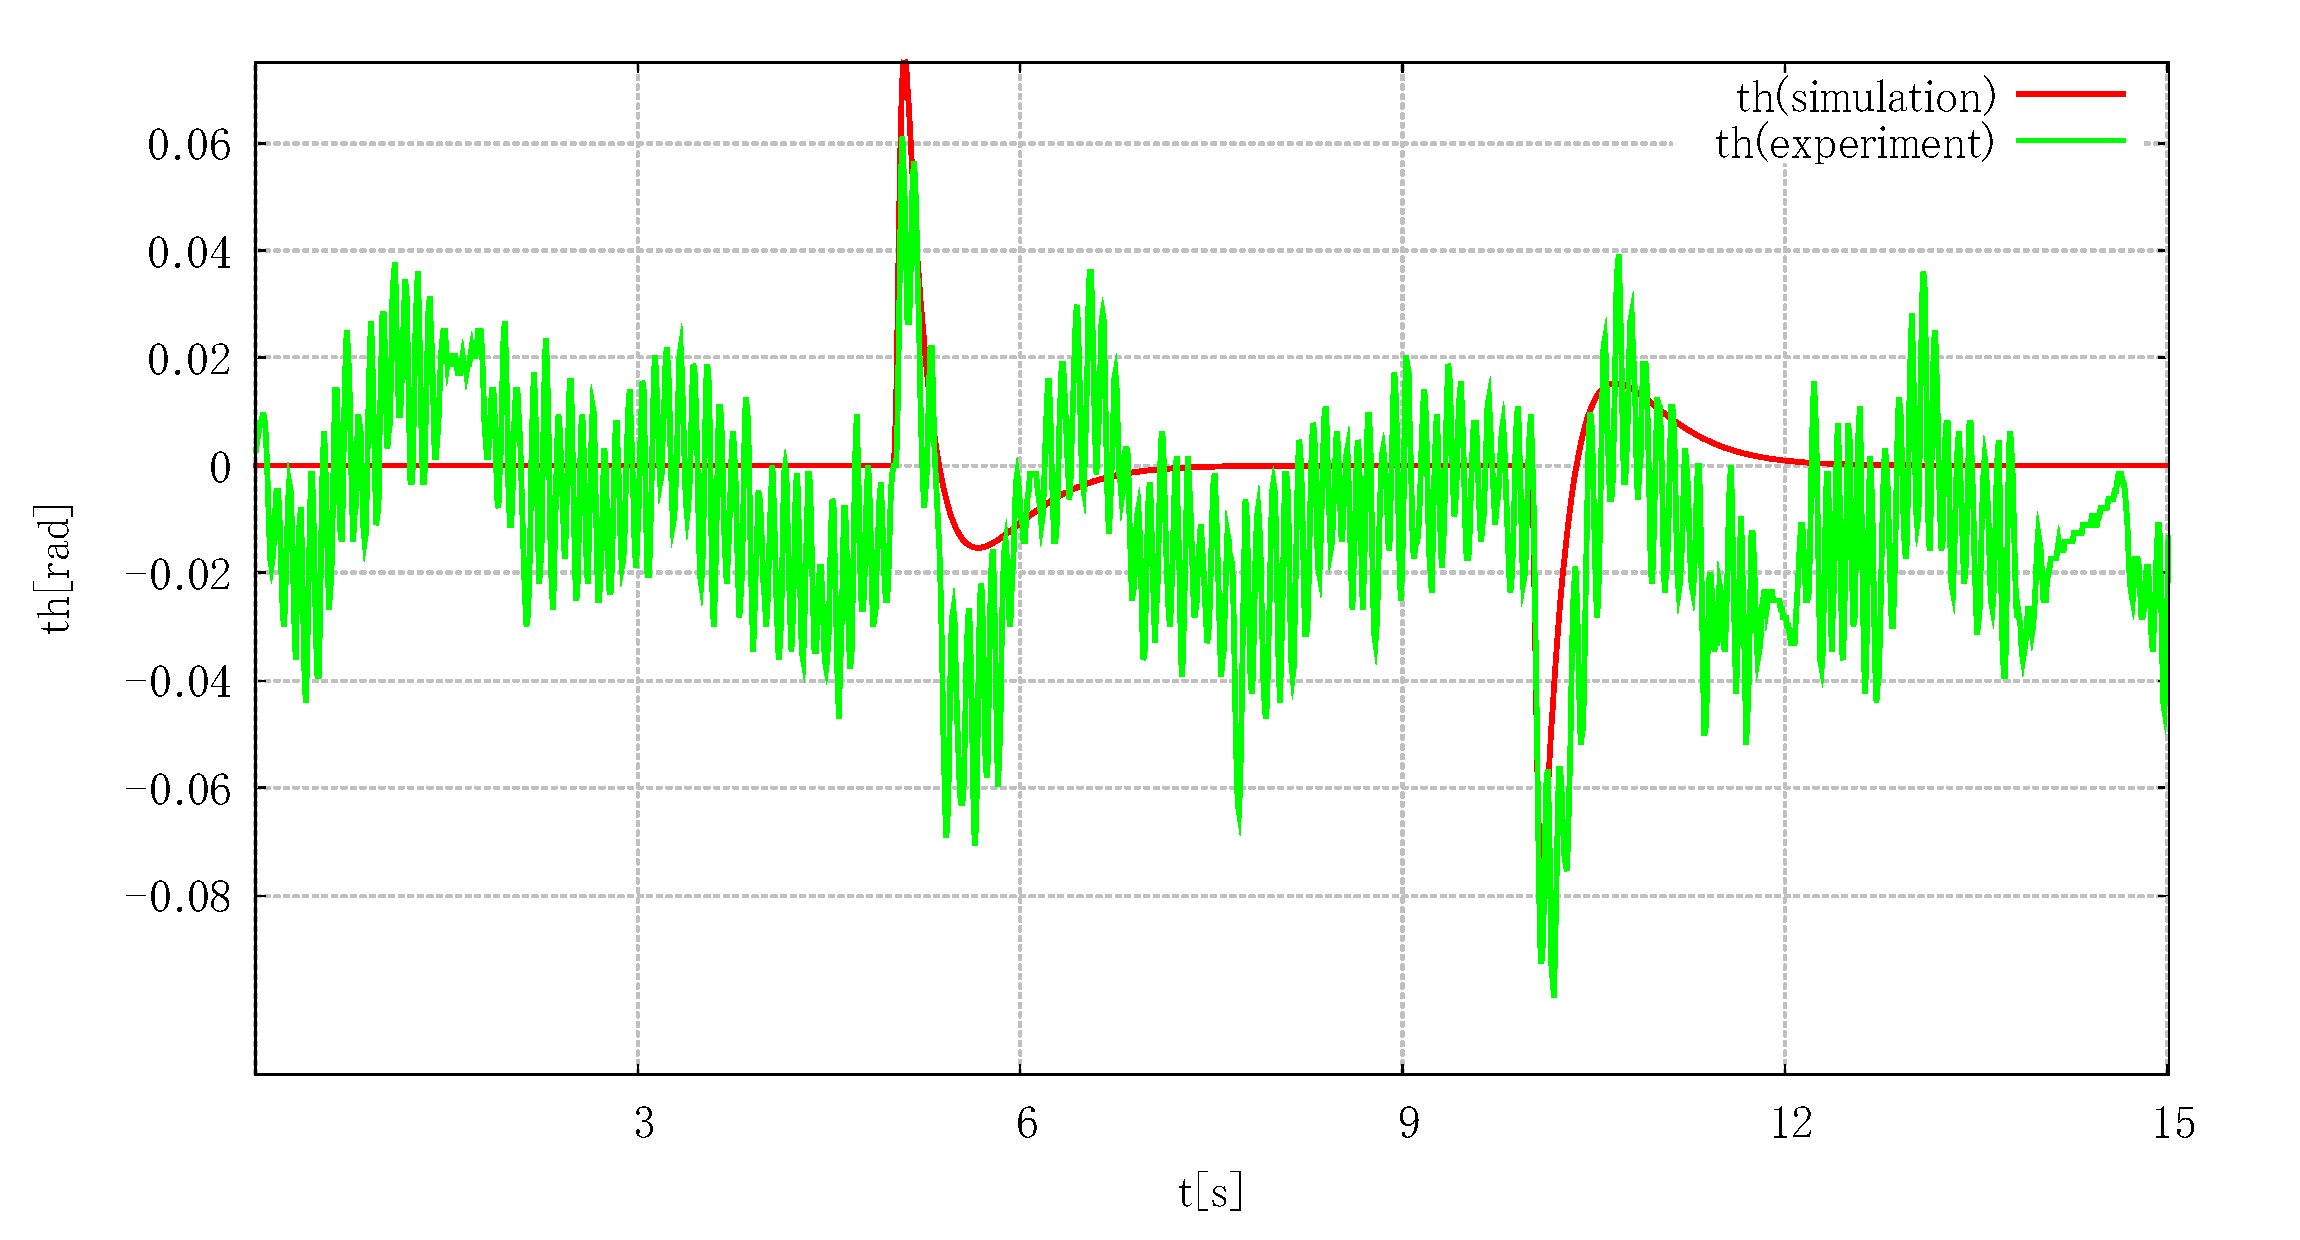
\includegraphics[width=0.4\linewidth]{gazo/experiment_Q55obs30dt10TH.eps}
		\caption{比較結果その7(左図がr,右図が$\theta$)}
		\label{image:sono7}
	\end{figure}
	\begin{figure}[H]
		\centering
		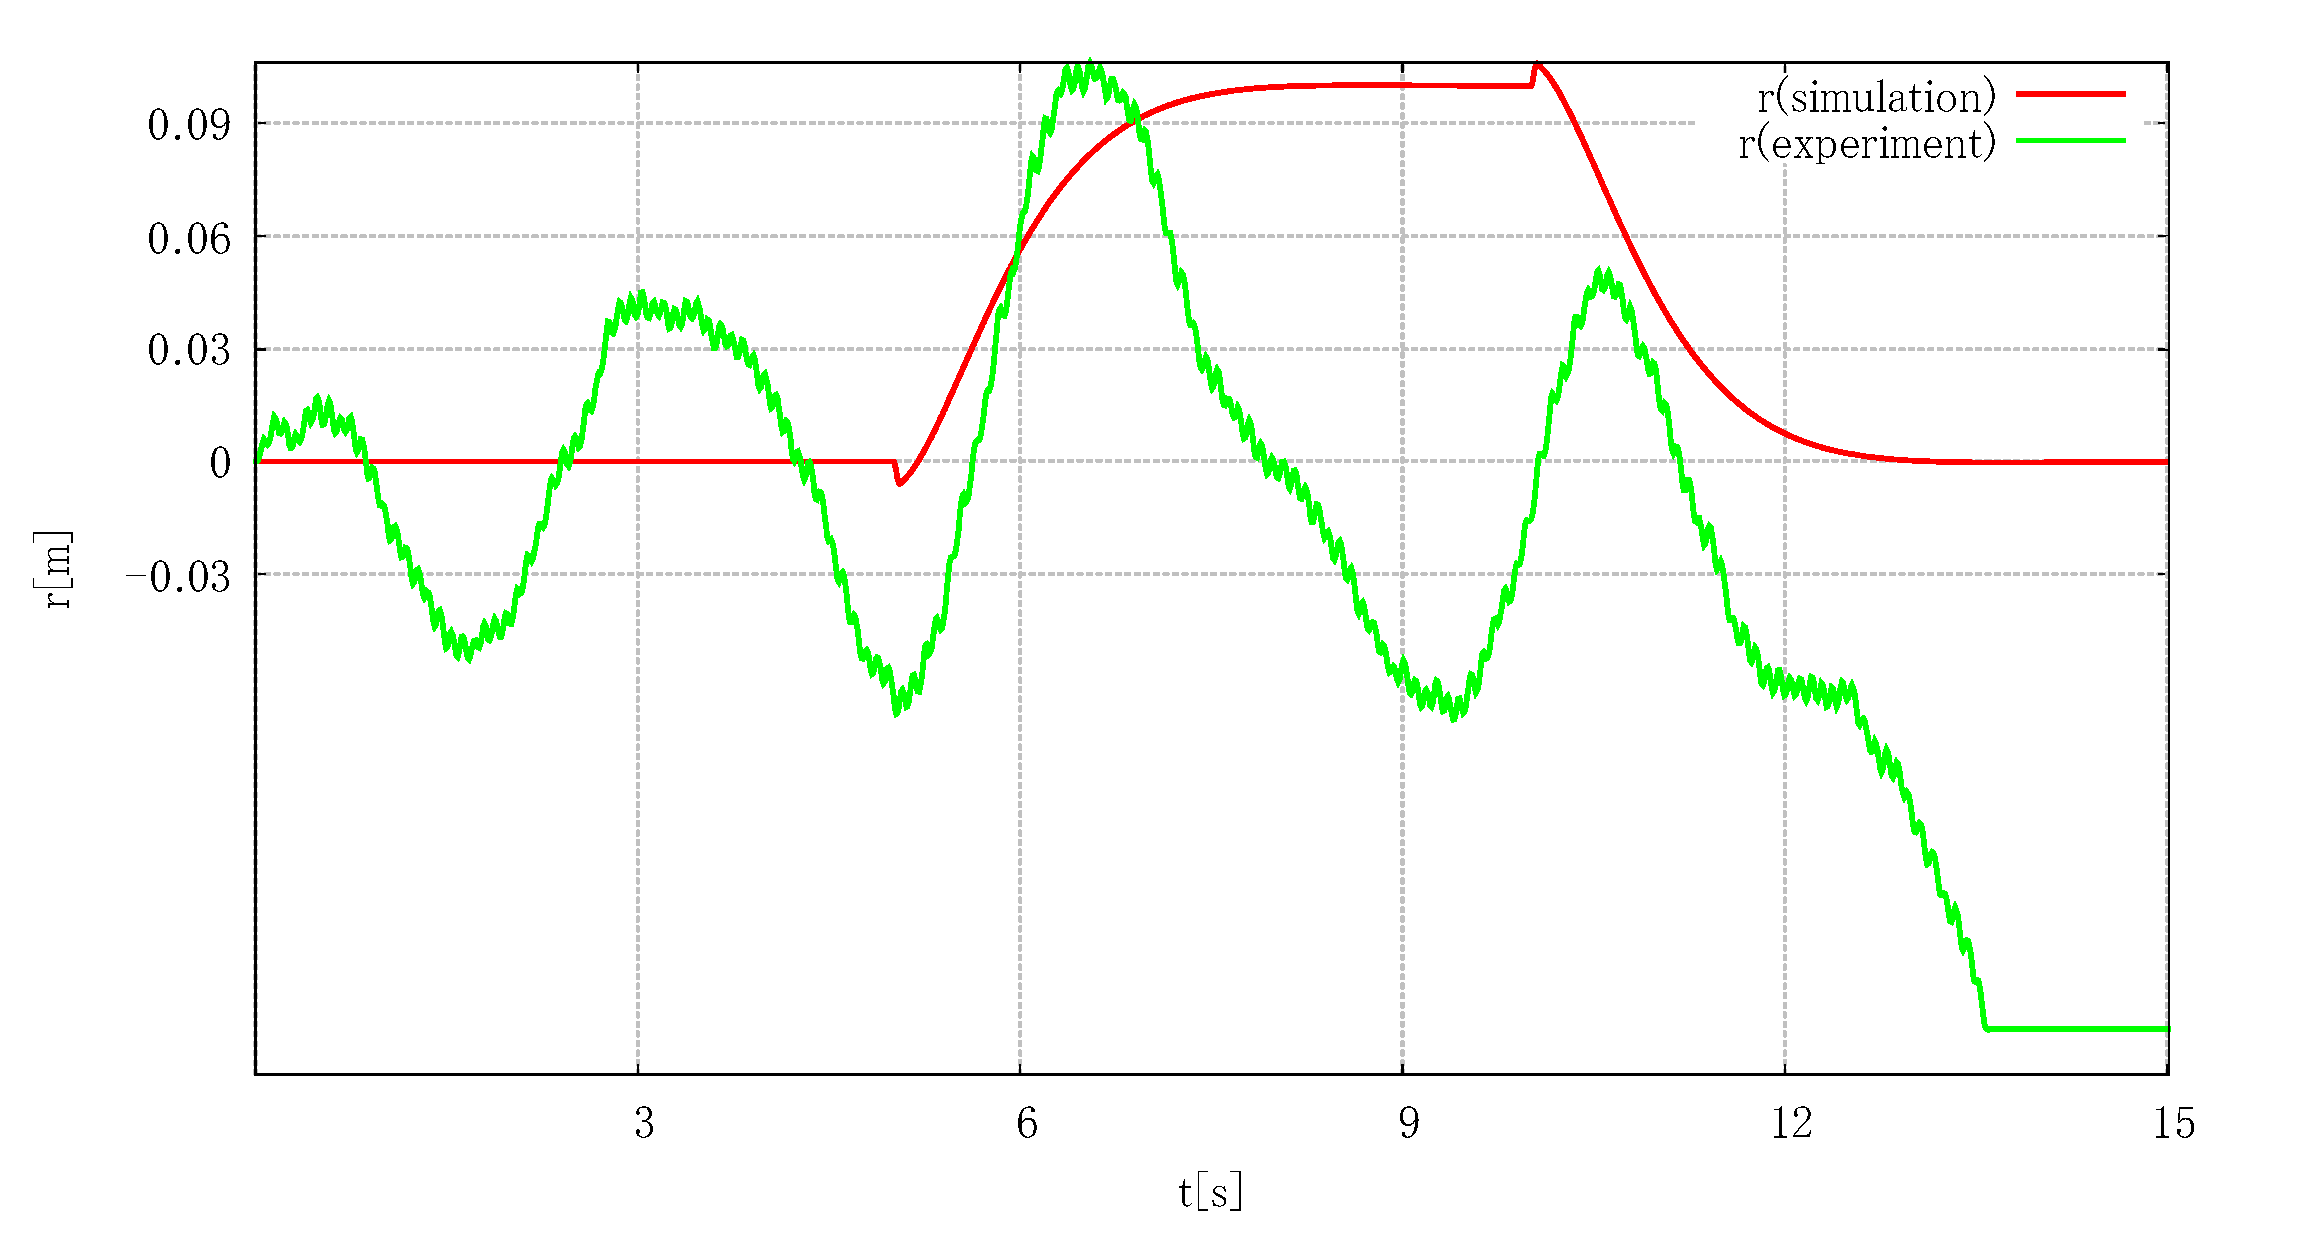
\includegraphics[width=0.4\linewidth]{gazo/experiment_Q56obs30dt10R.eps}
		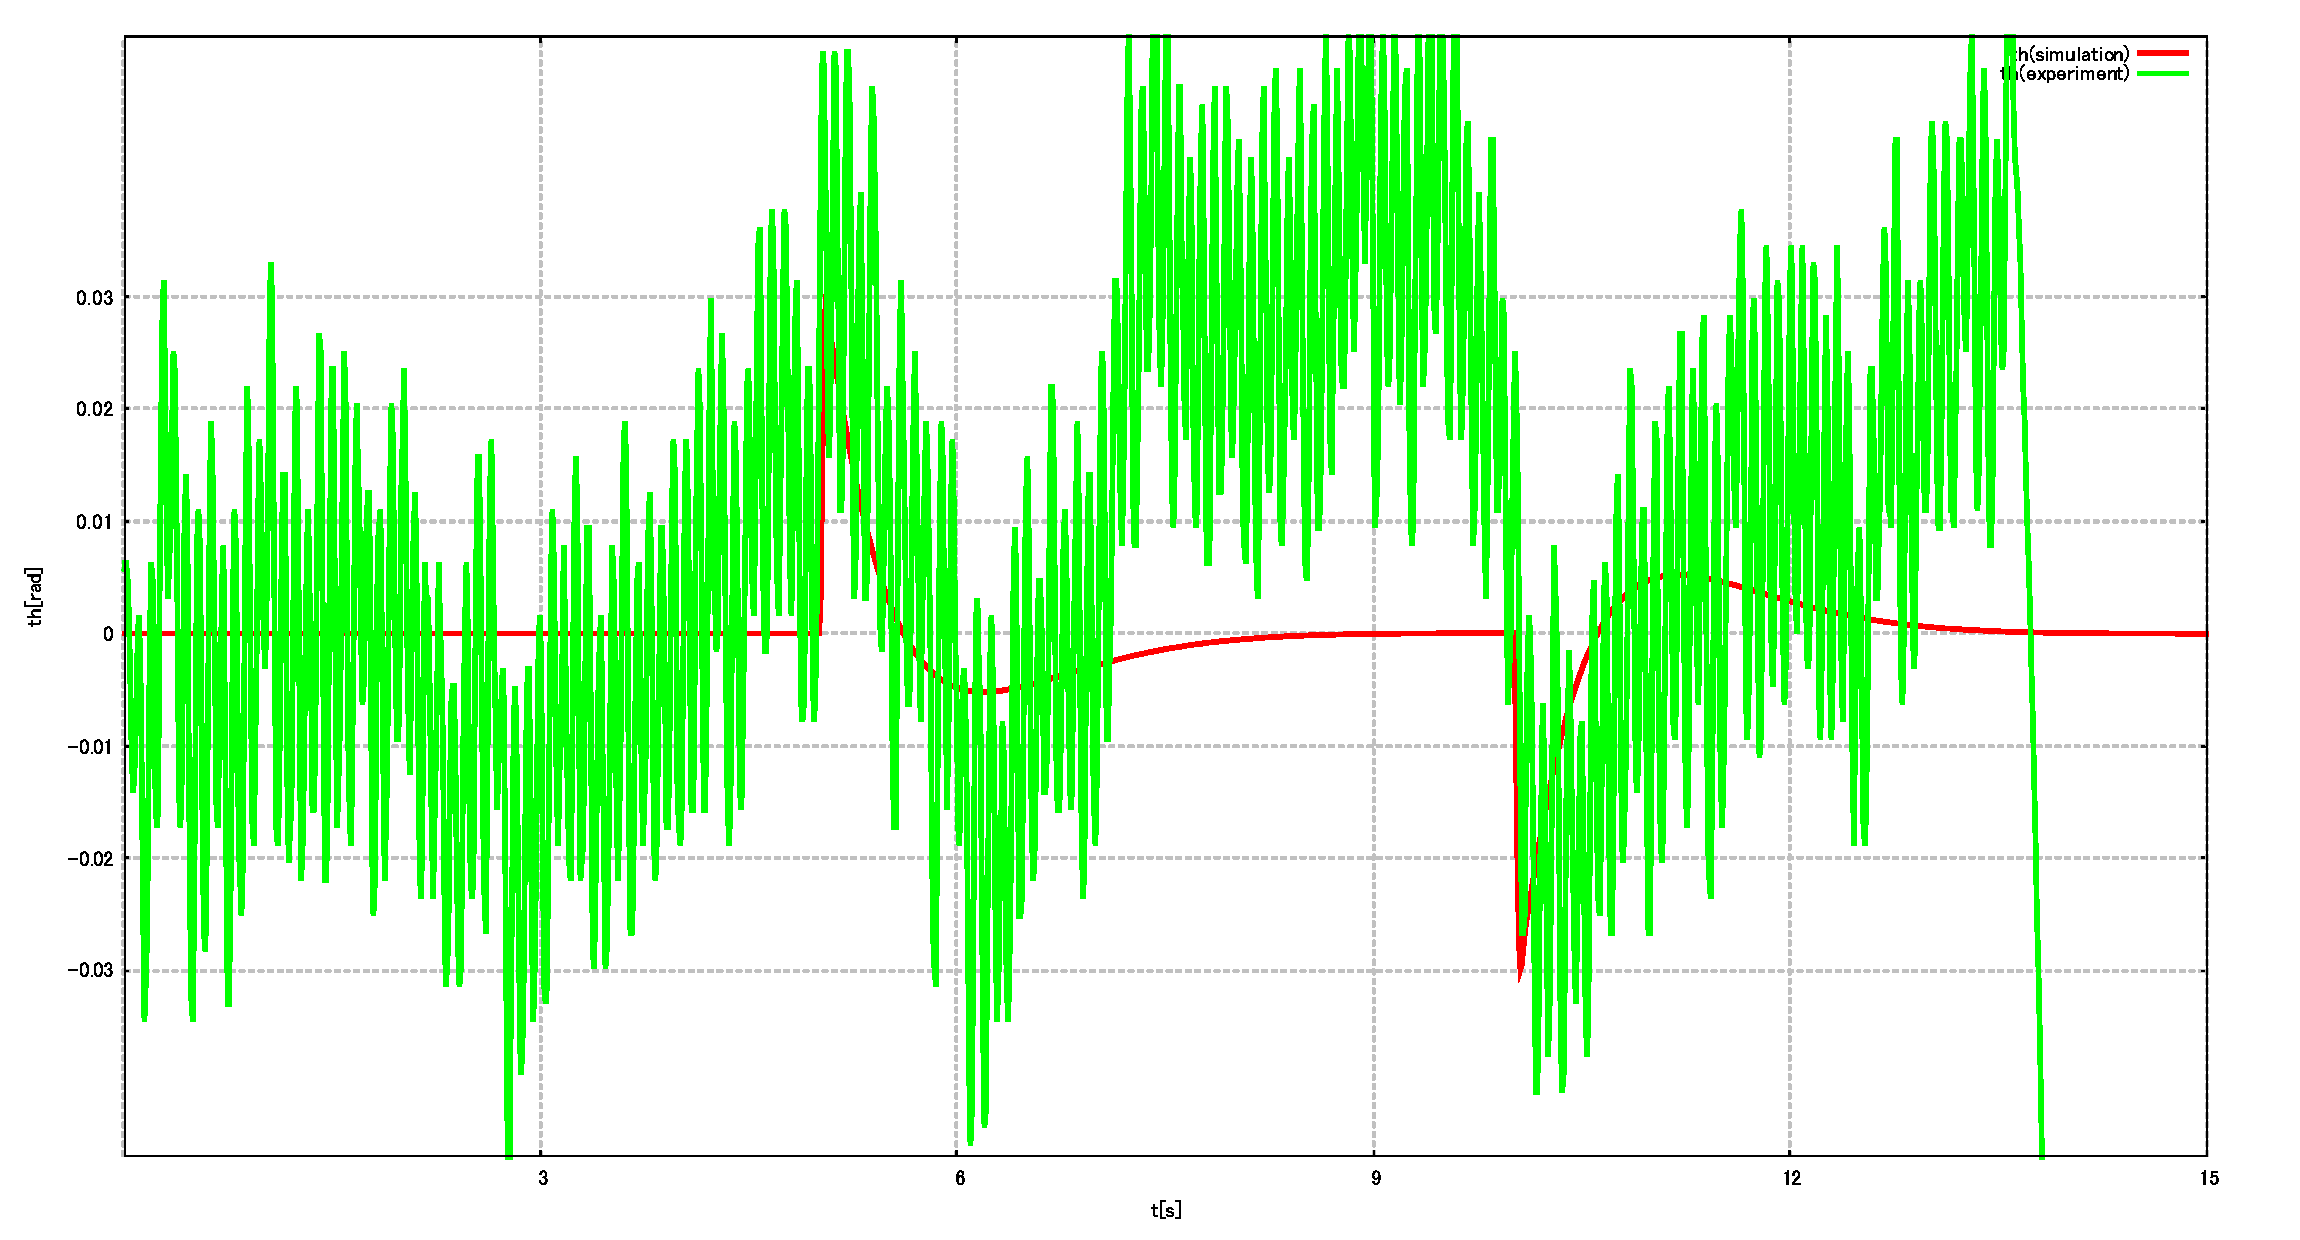
\includegraphics[width=0.4\linewidth]{gazo/experiment_Q56obs30dt10TH.eps}
		\caption{比較結果その8(左図がr,右図が$\theta$)}
		\label{image:sono8}
	\end{figure}
	\begin{figure}[H]
		\centering
		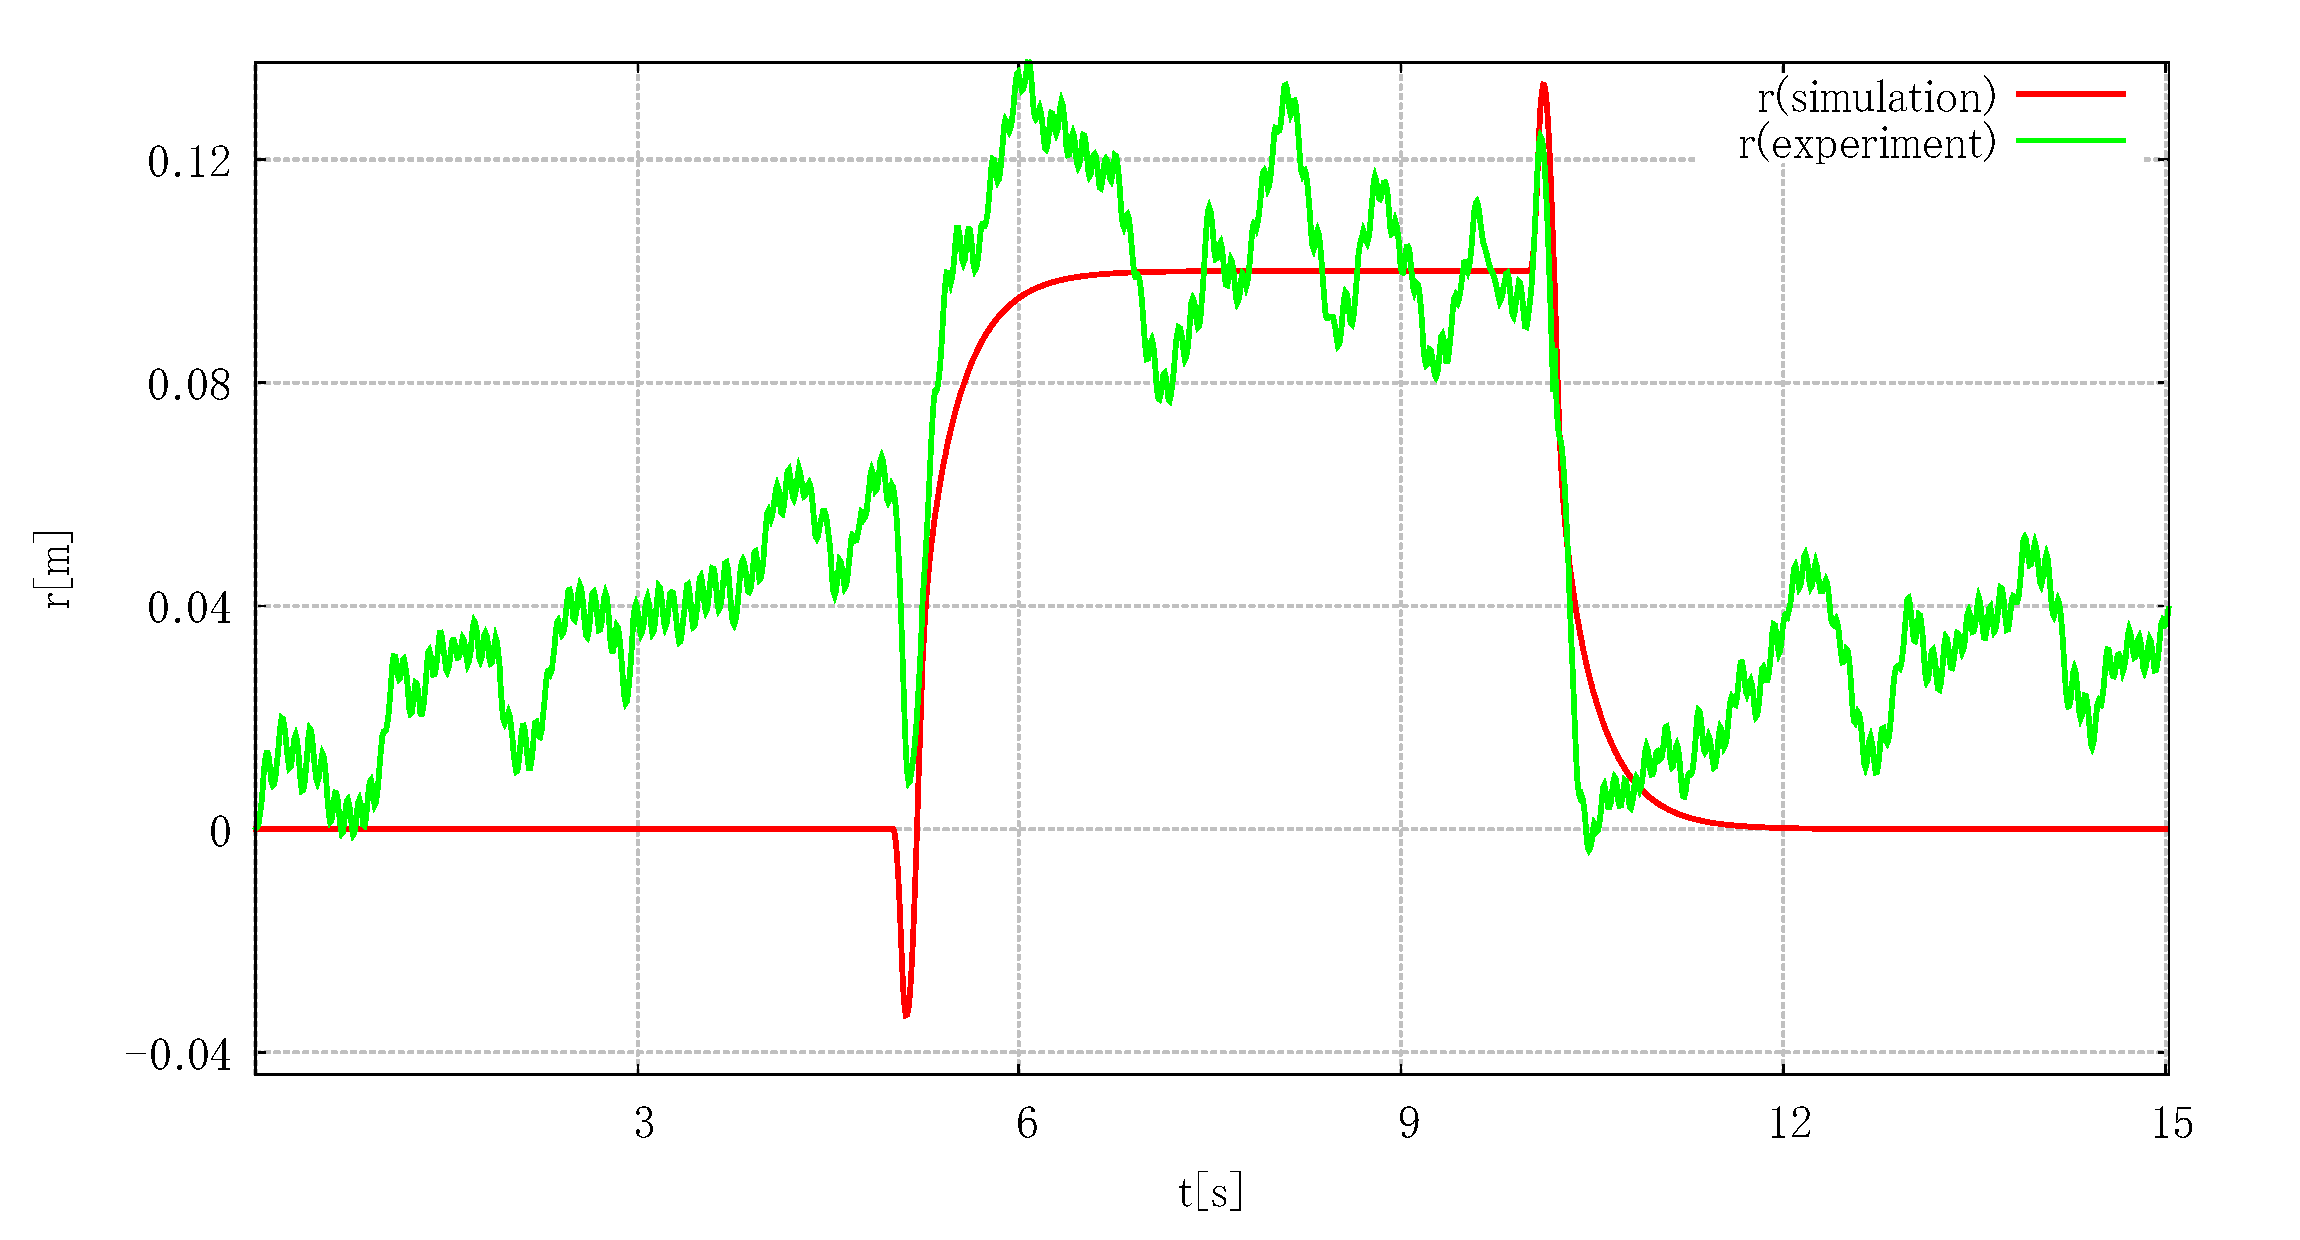
\includegraphics[width=0.4\linewidth]{gazo/experiment_Q65obs30dt10R.eps}
		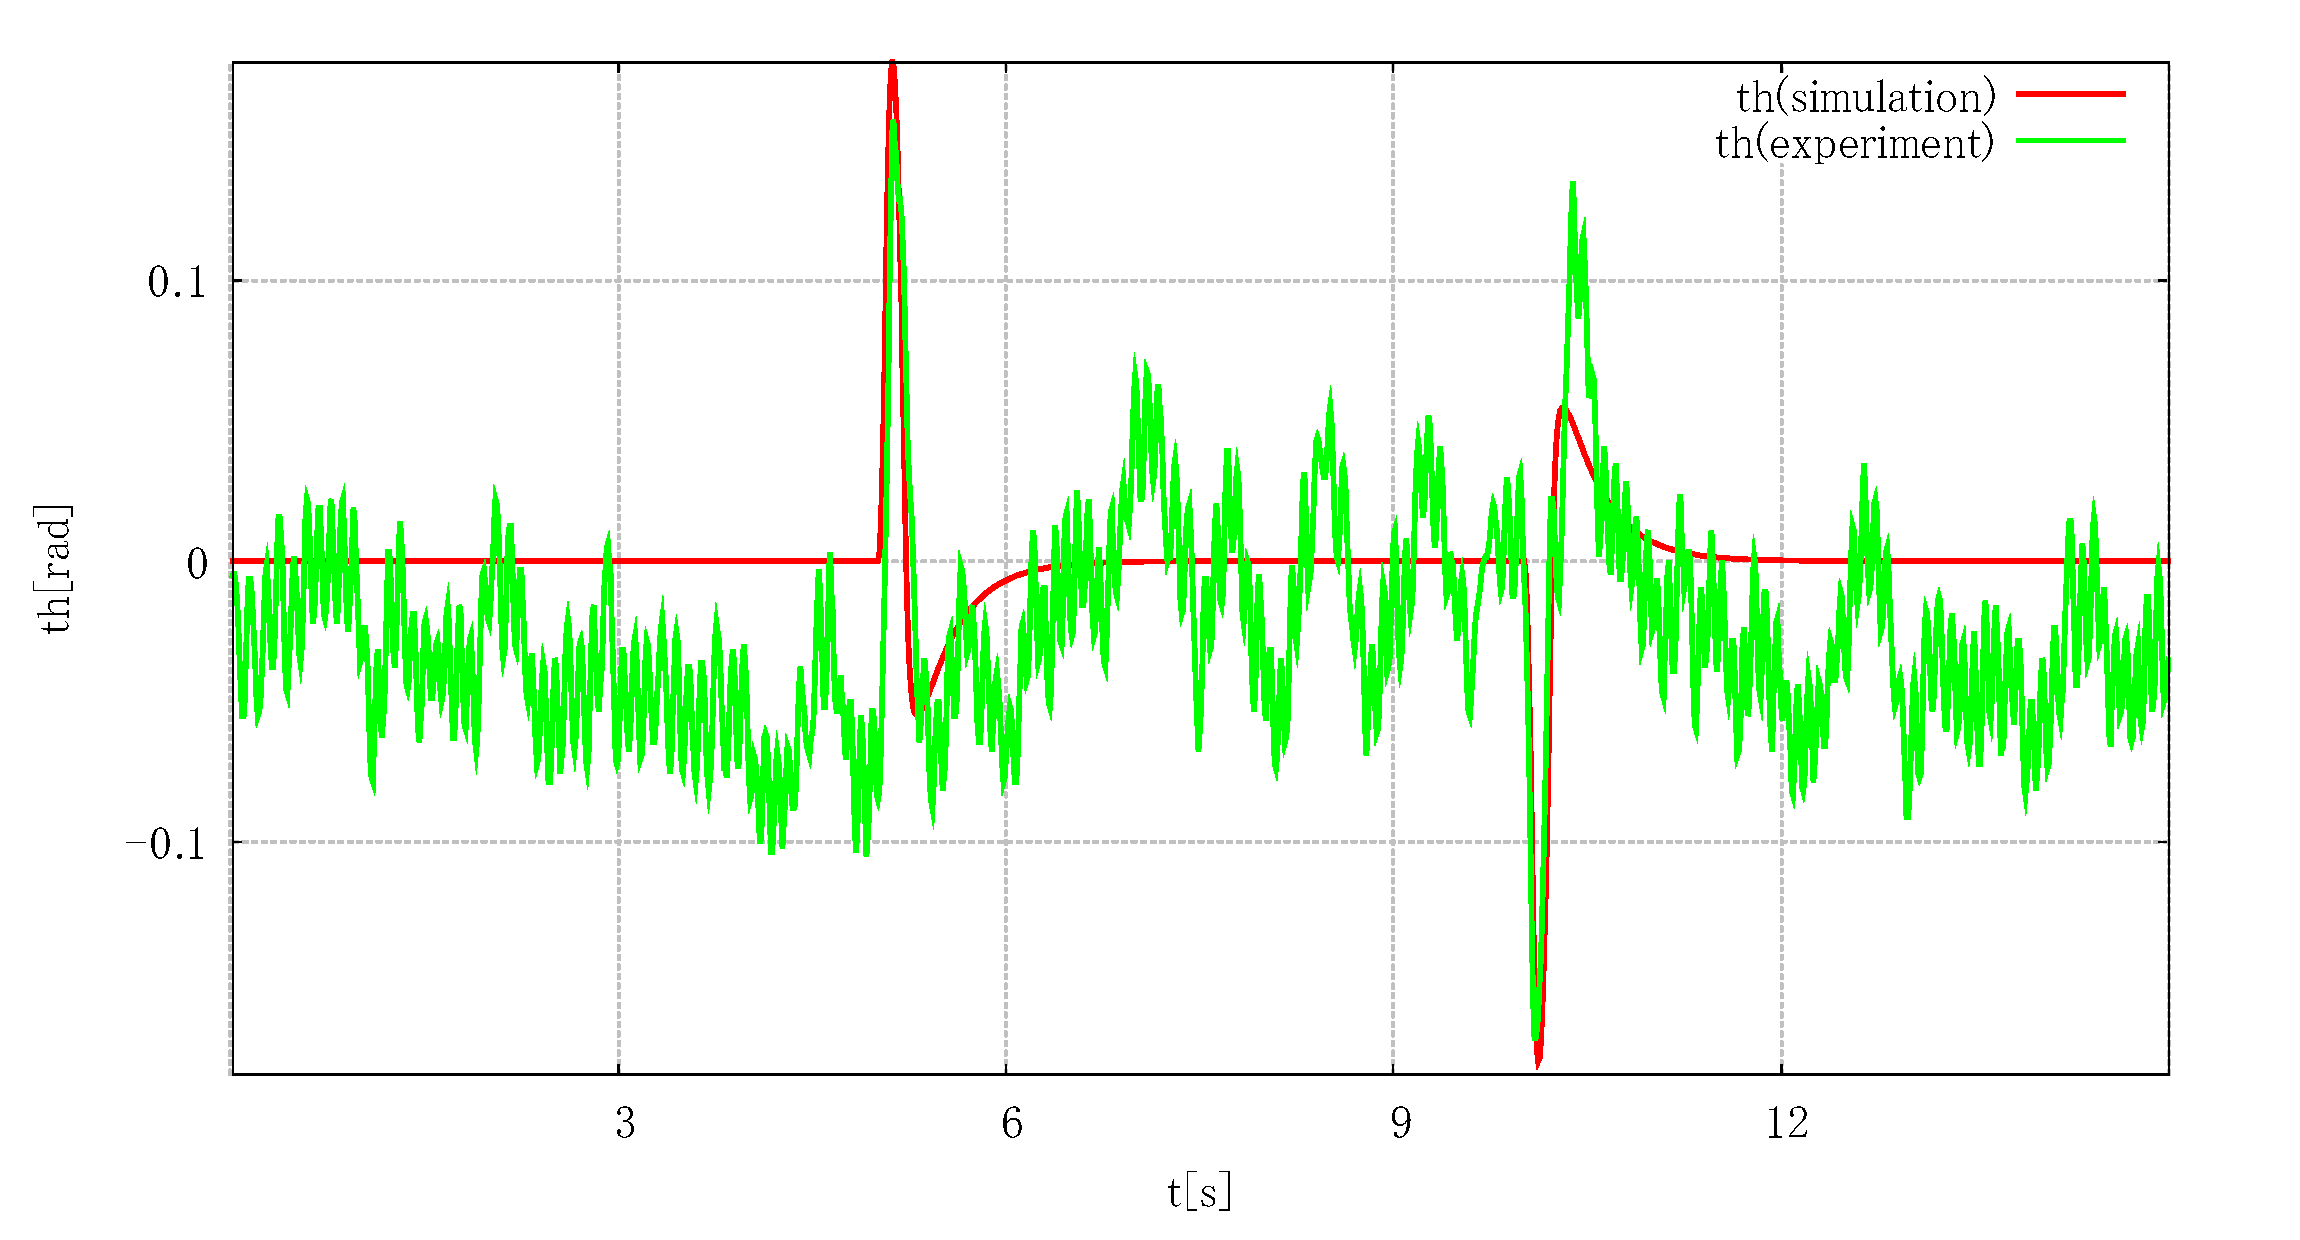
\includegraphics[width=0.4\linewidth]{gazo/experiment_Q65obs30dt10TH.eps}
		\caption{比較結果その9(左図がr,右図が$\theta$)}
		\label{image:sono9}
	\end{figure}
	\begin{figure}[H]
		\centering
		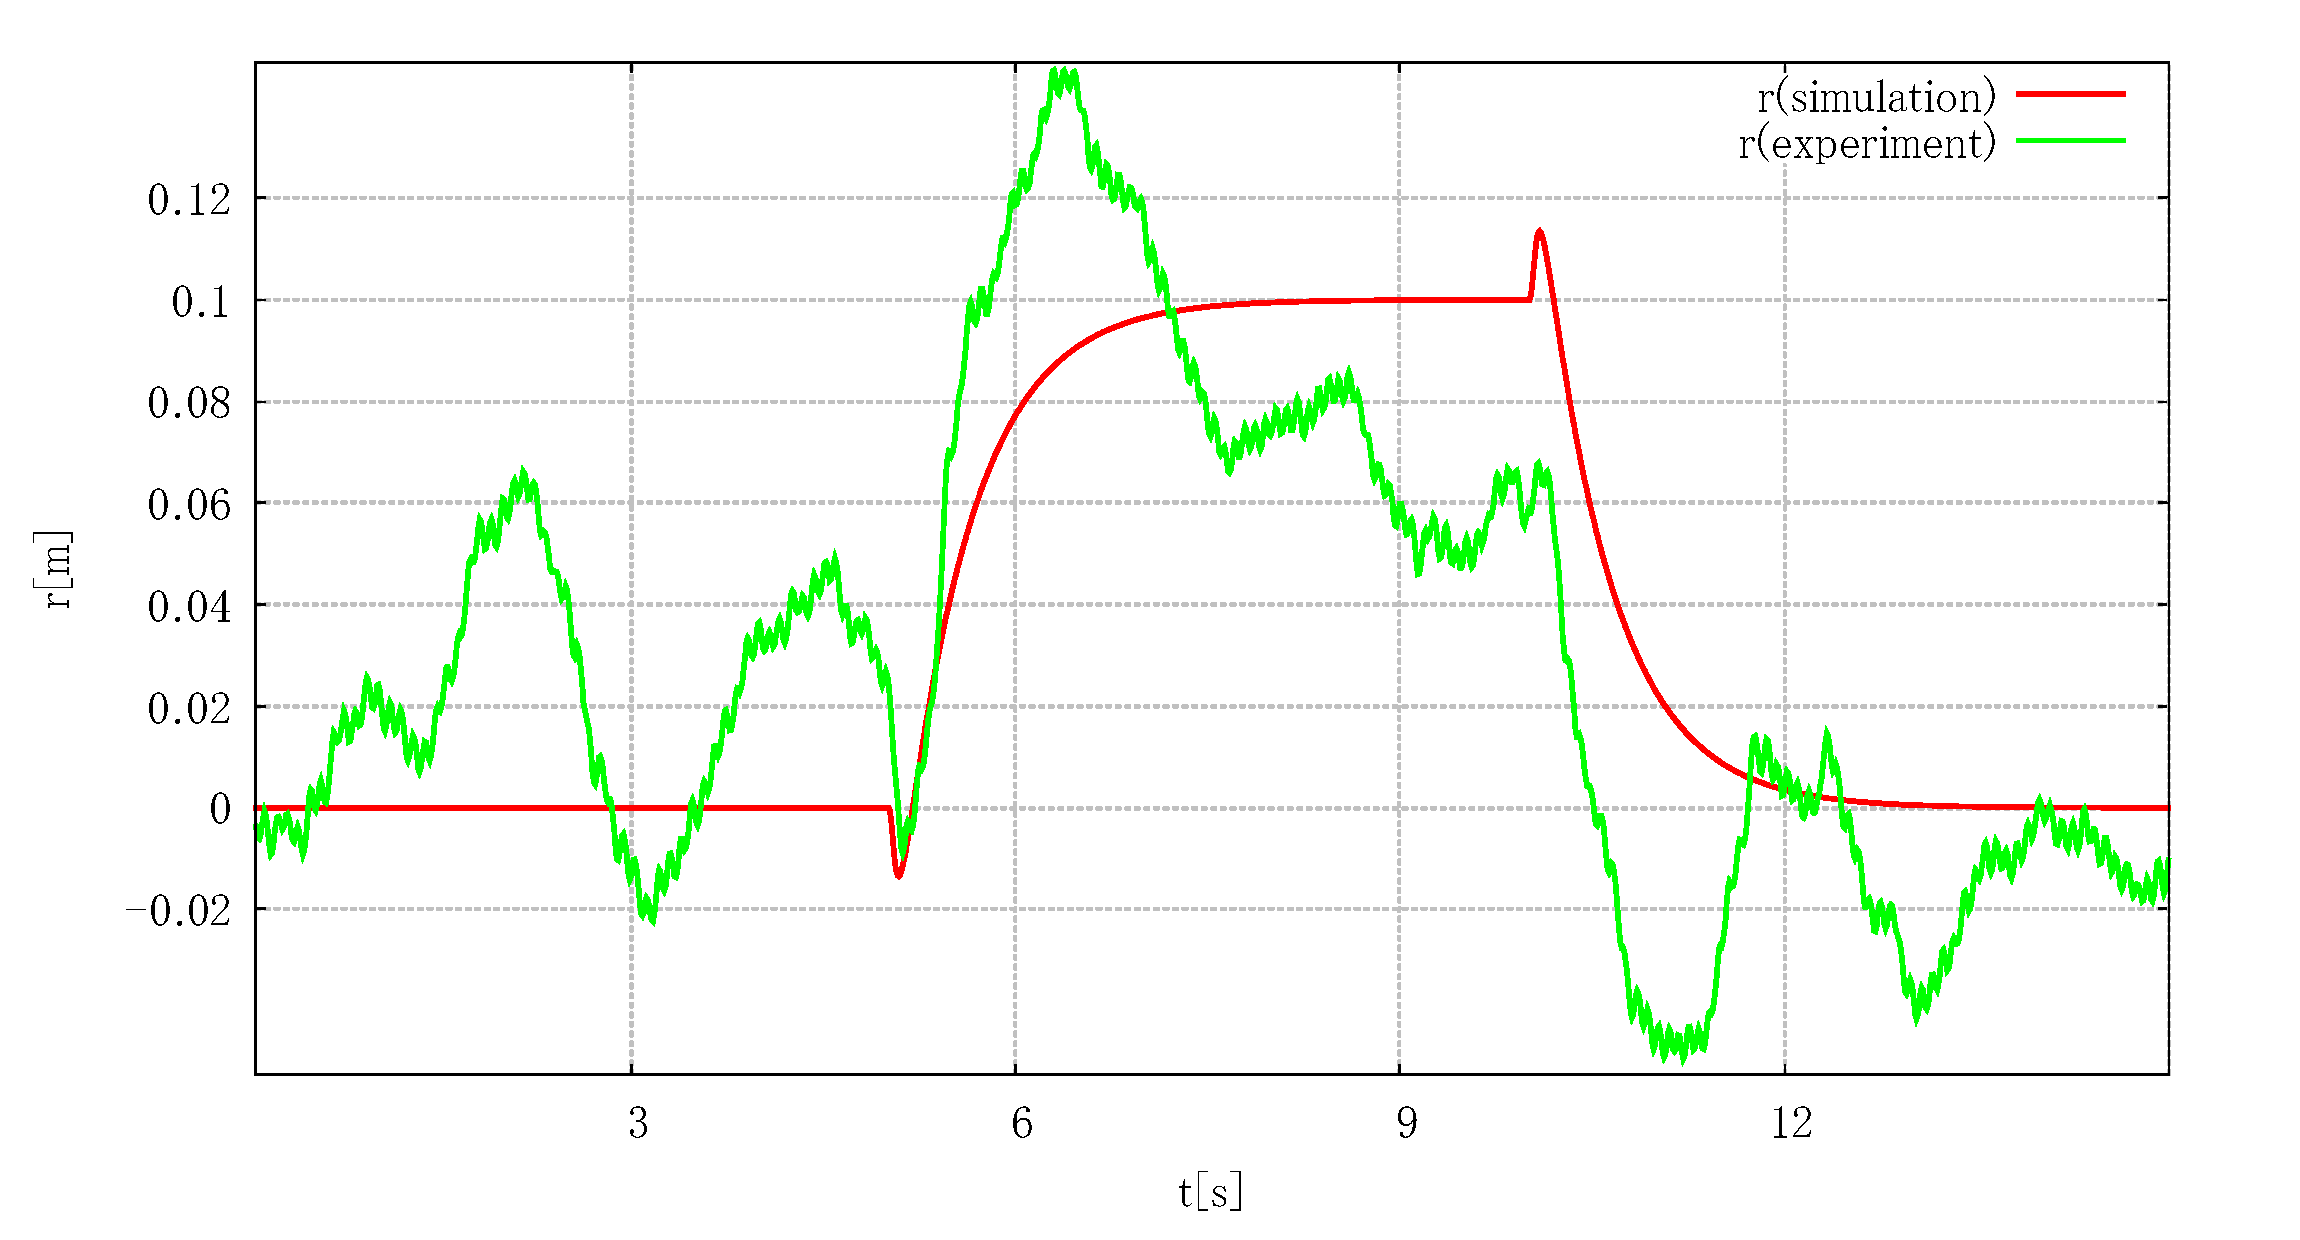
\includegraphics[width=0.4\linewidth]{gazo/experiment_Q55obs60dt10R.eps}
		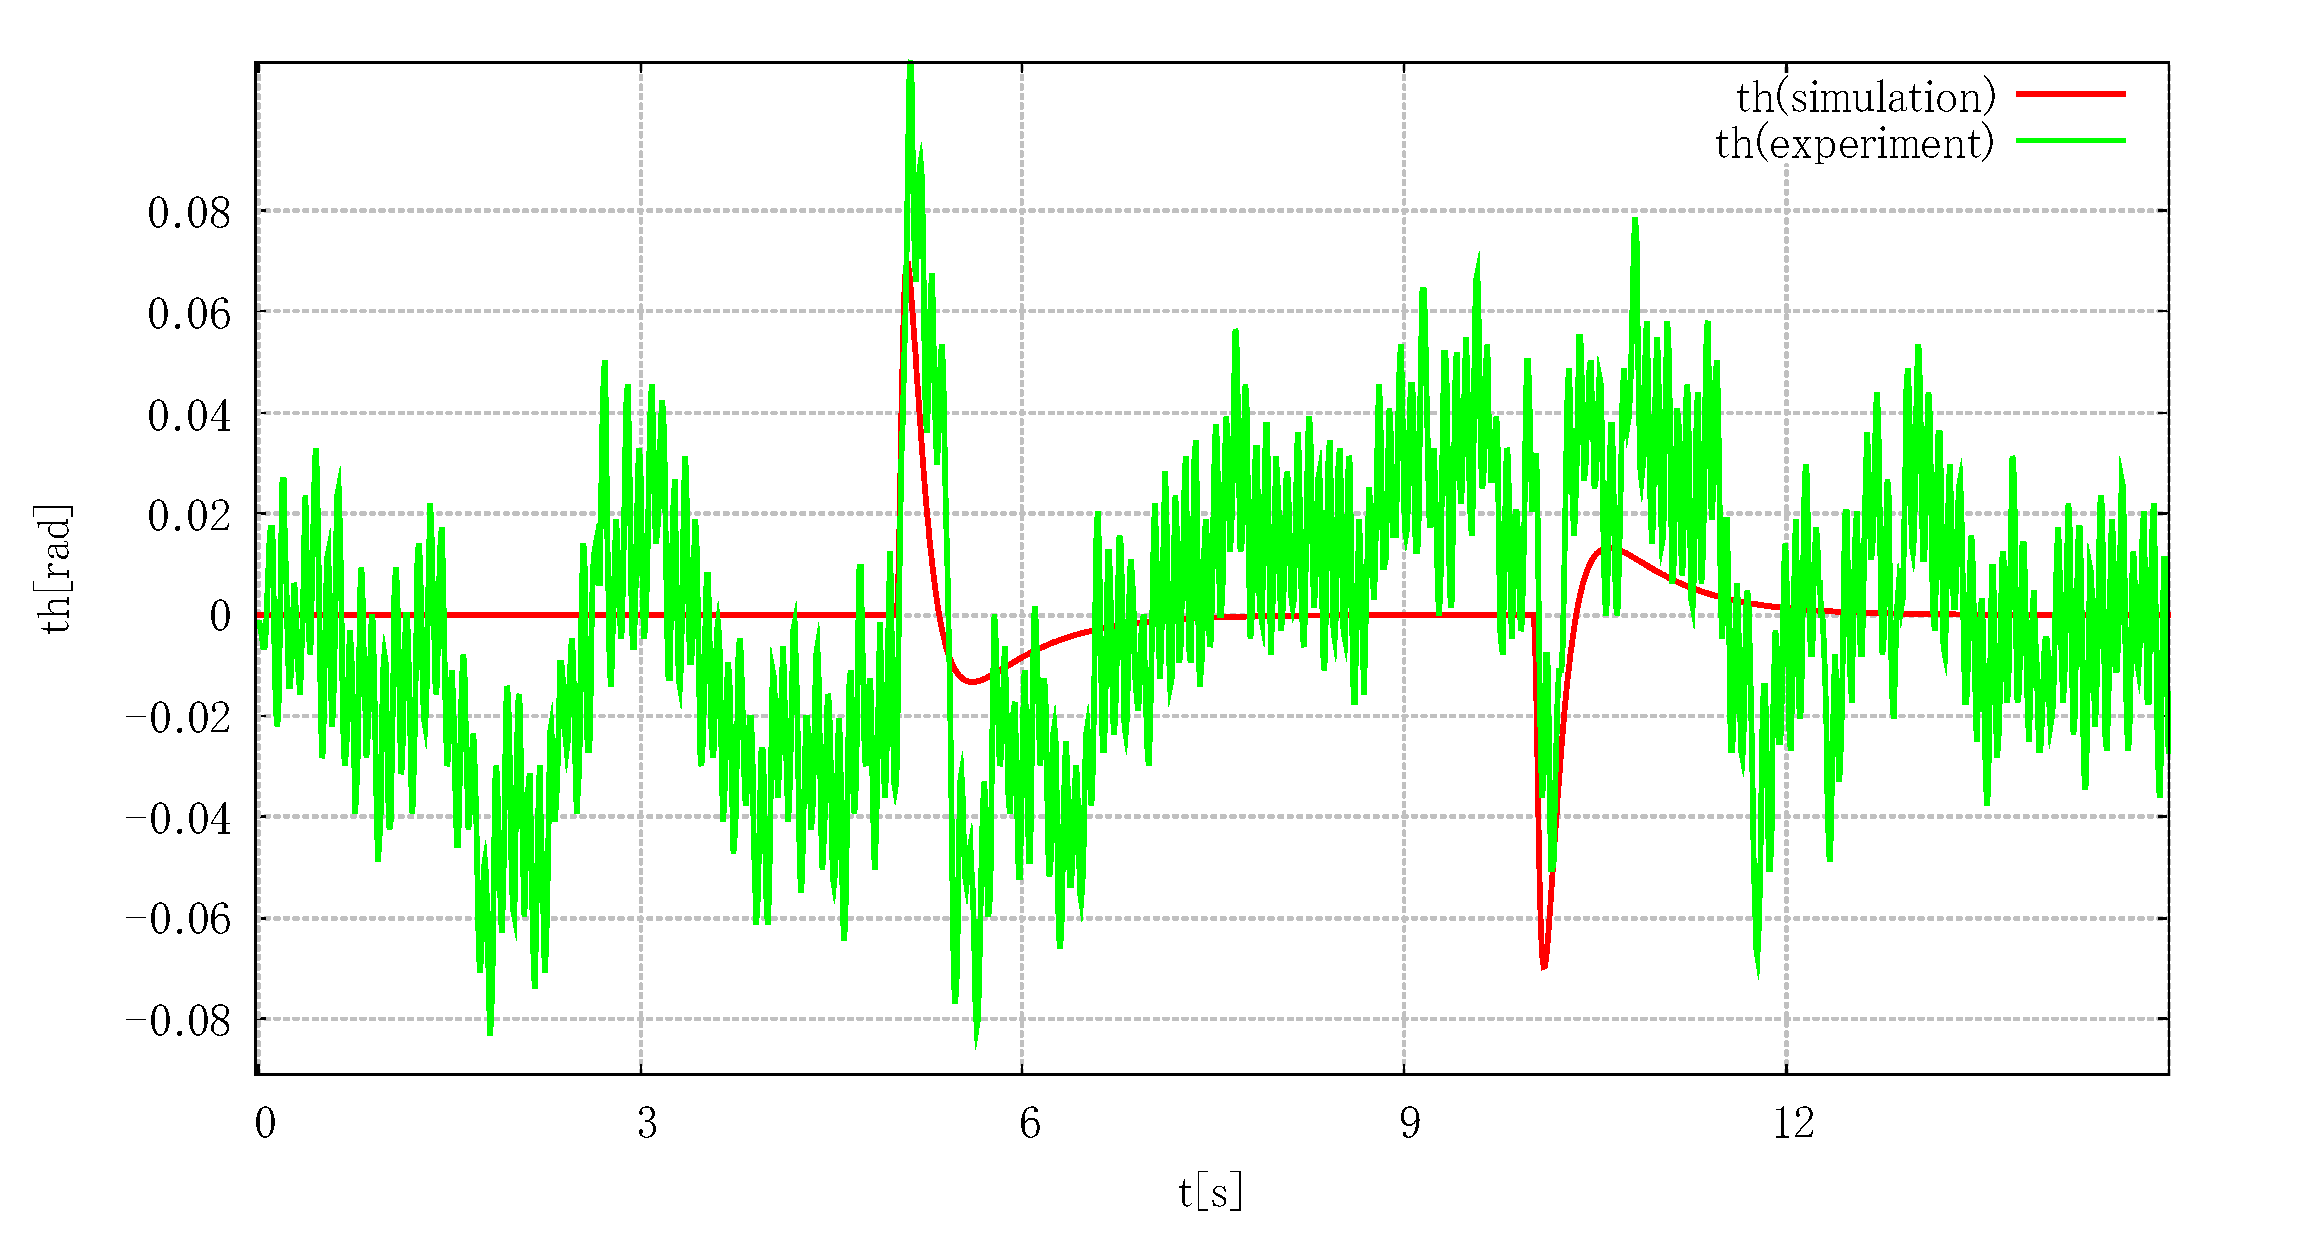
\includegraphics[width=0.4\linewidth]{gazo/experiment_Q55obs60dt10TH.eps}
		\caption{比較結果その10(左図がr,右図が$\theta$)}
		\label{image:sono10}
	\end{figure}
	\begin{figure}[H]
		\centering
		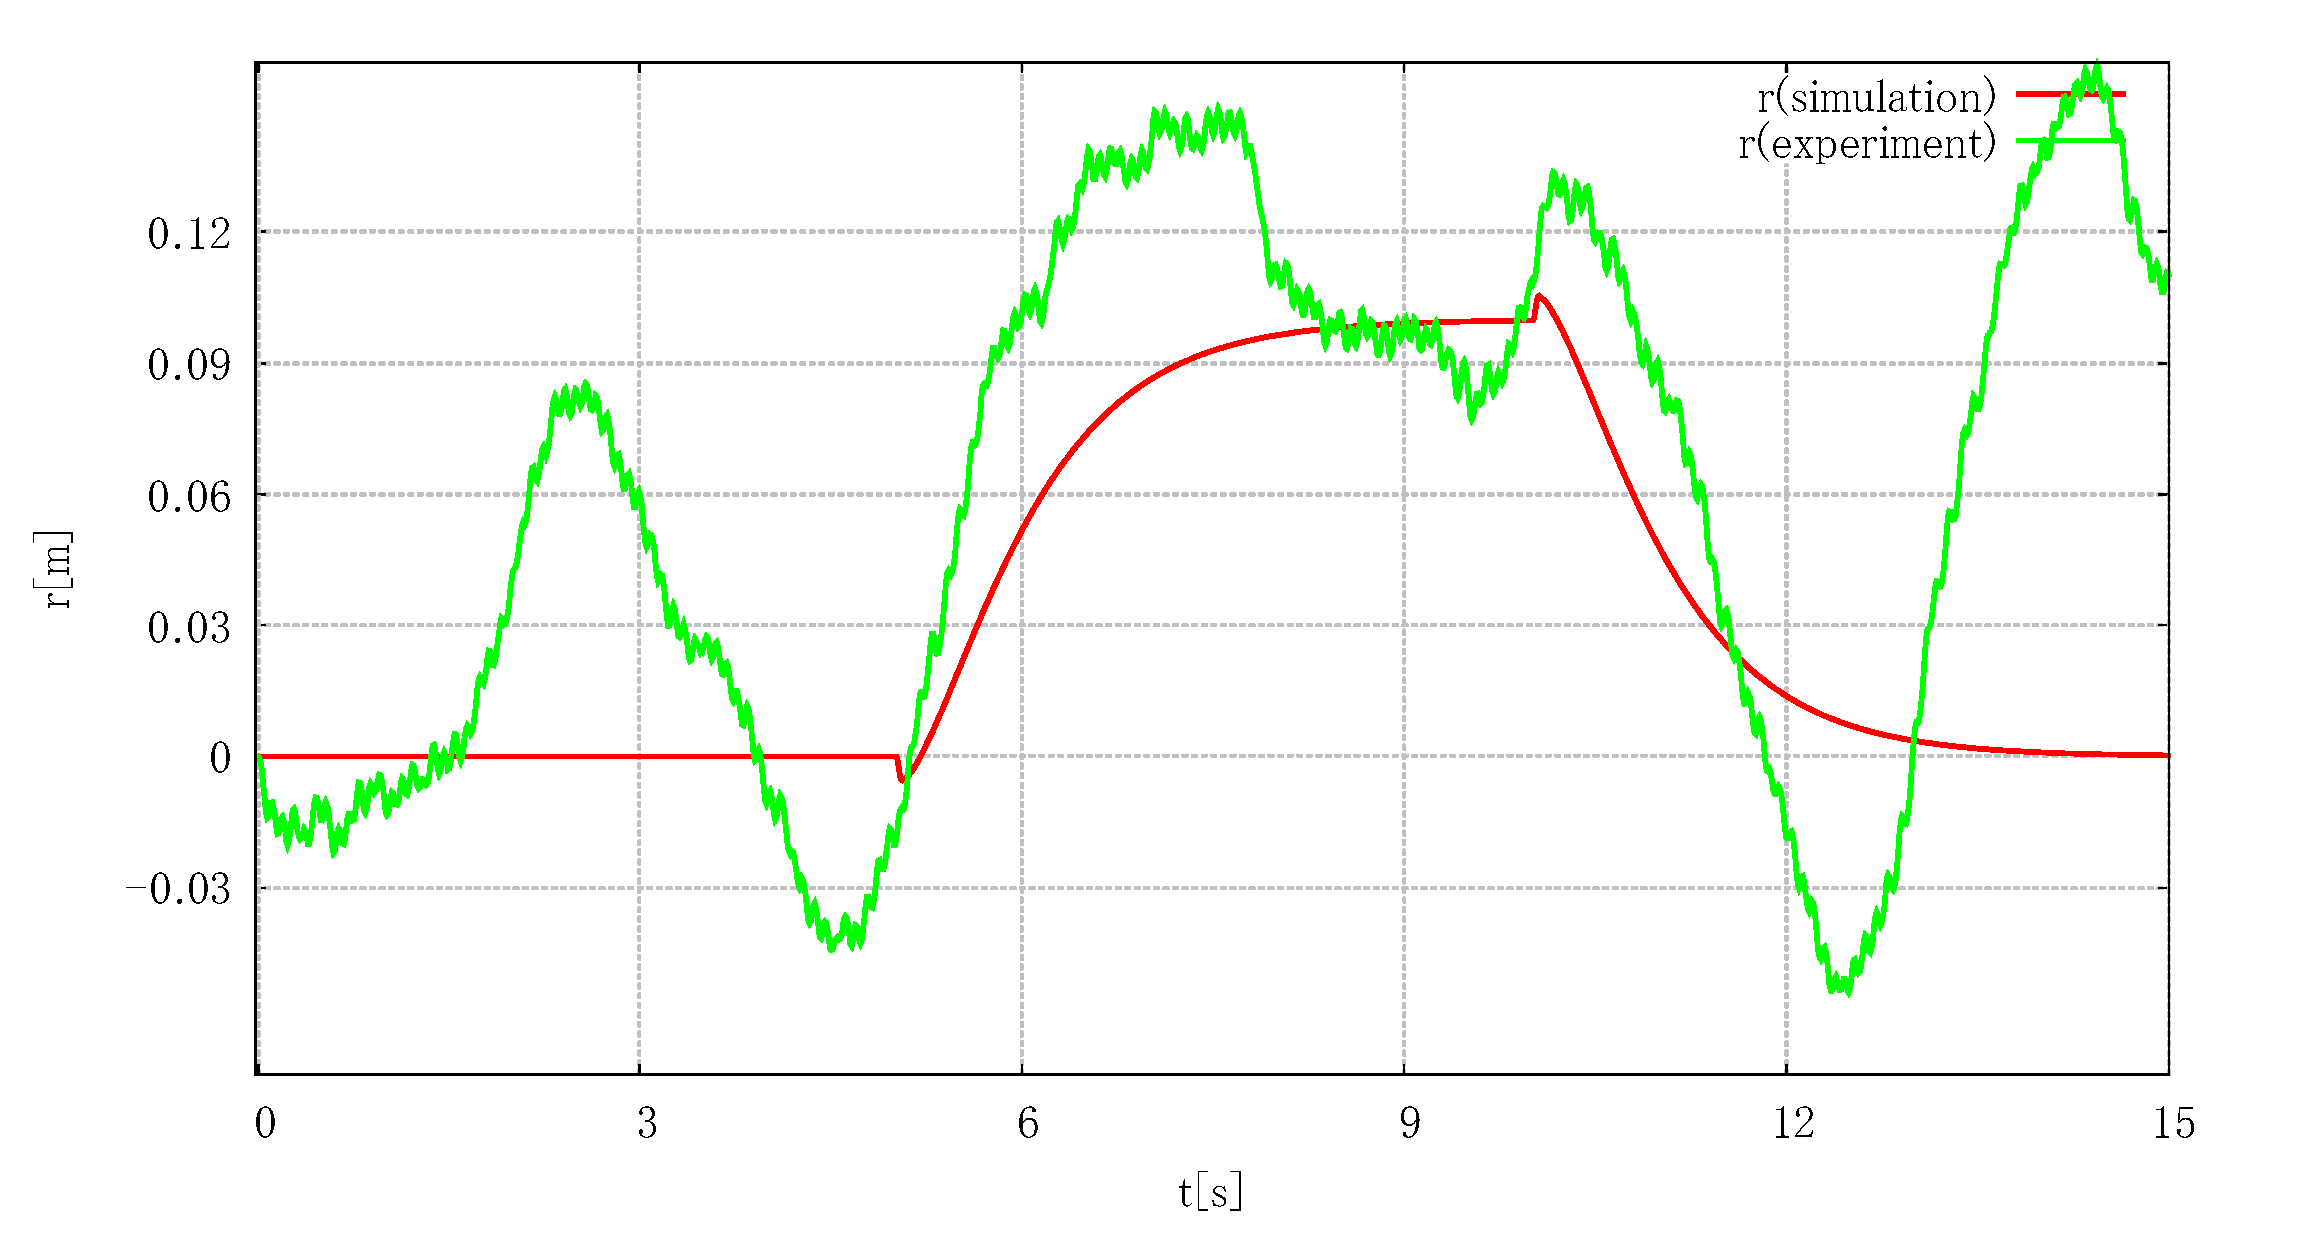
\includegraphics[width=0.4\linewidth]{gazo/experiment_Q56obs60dt10R.eps}
		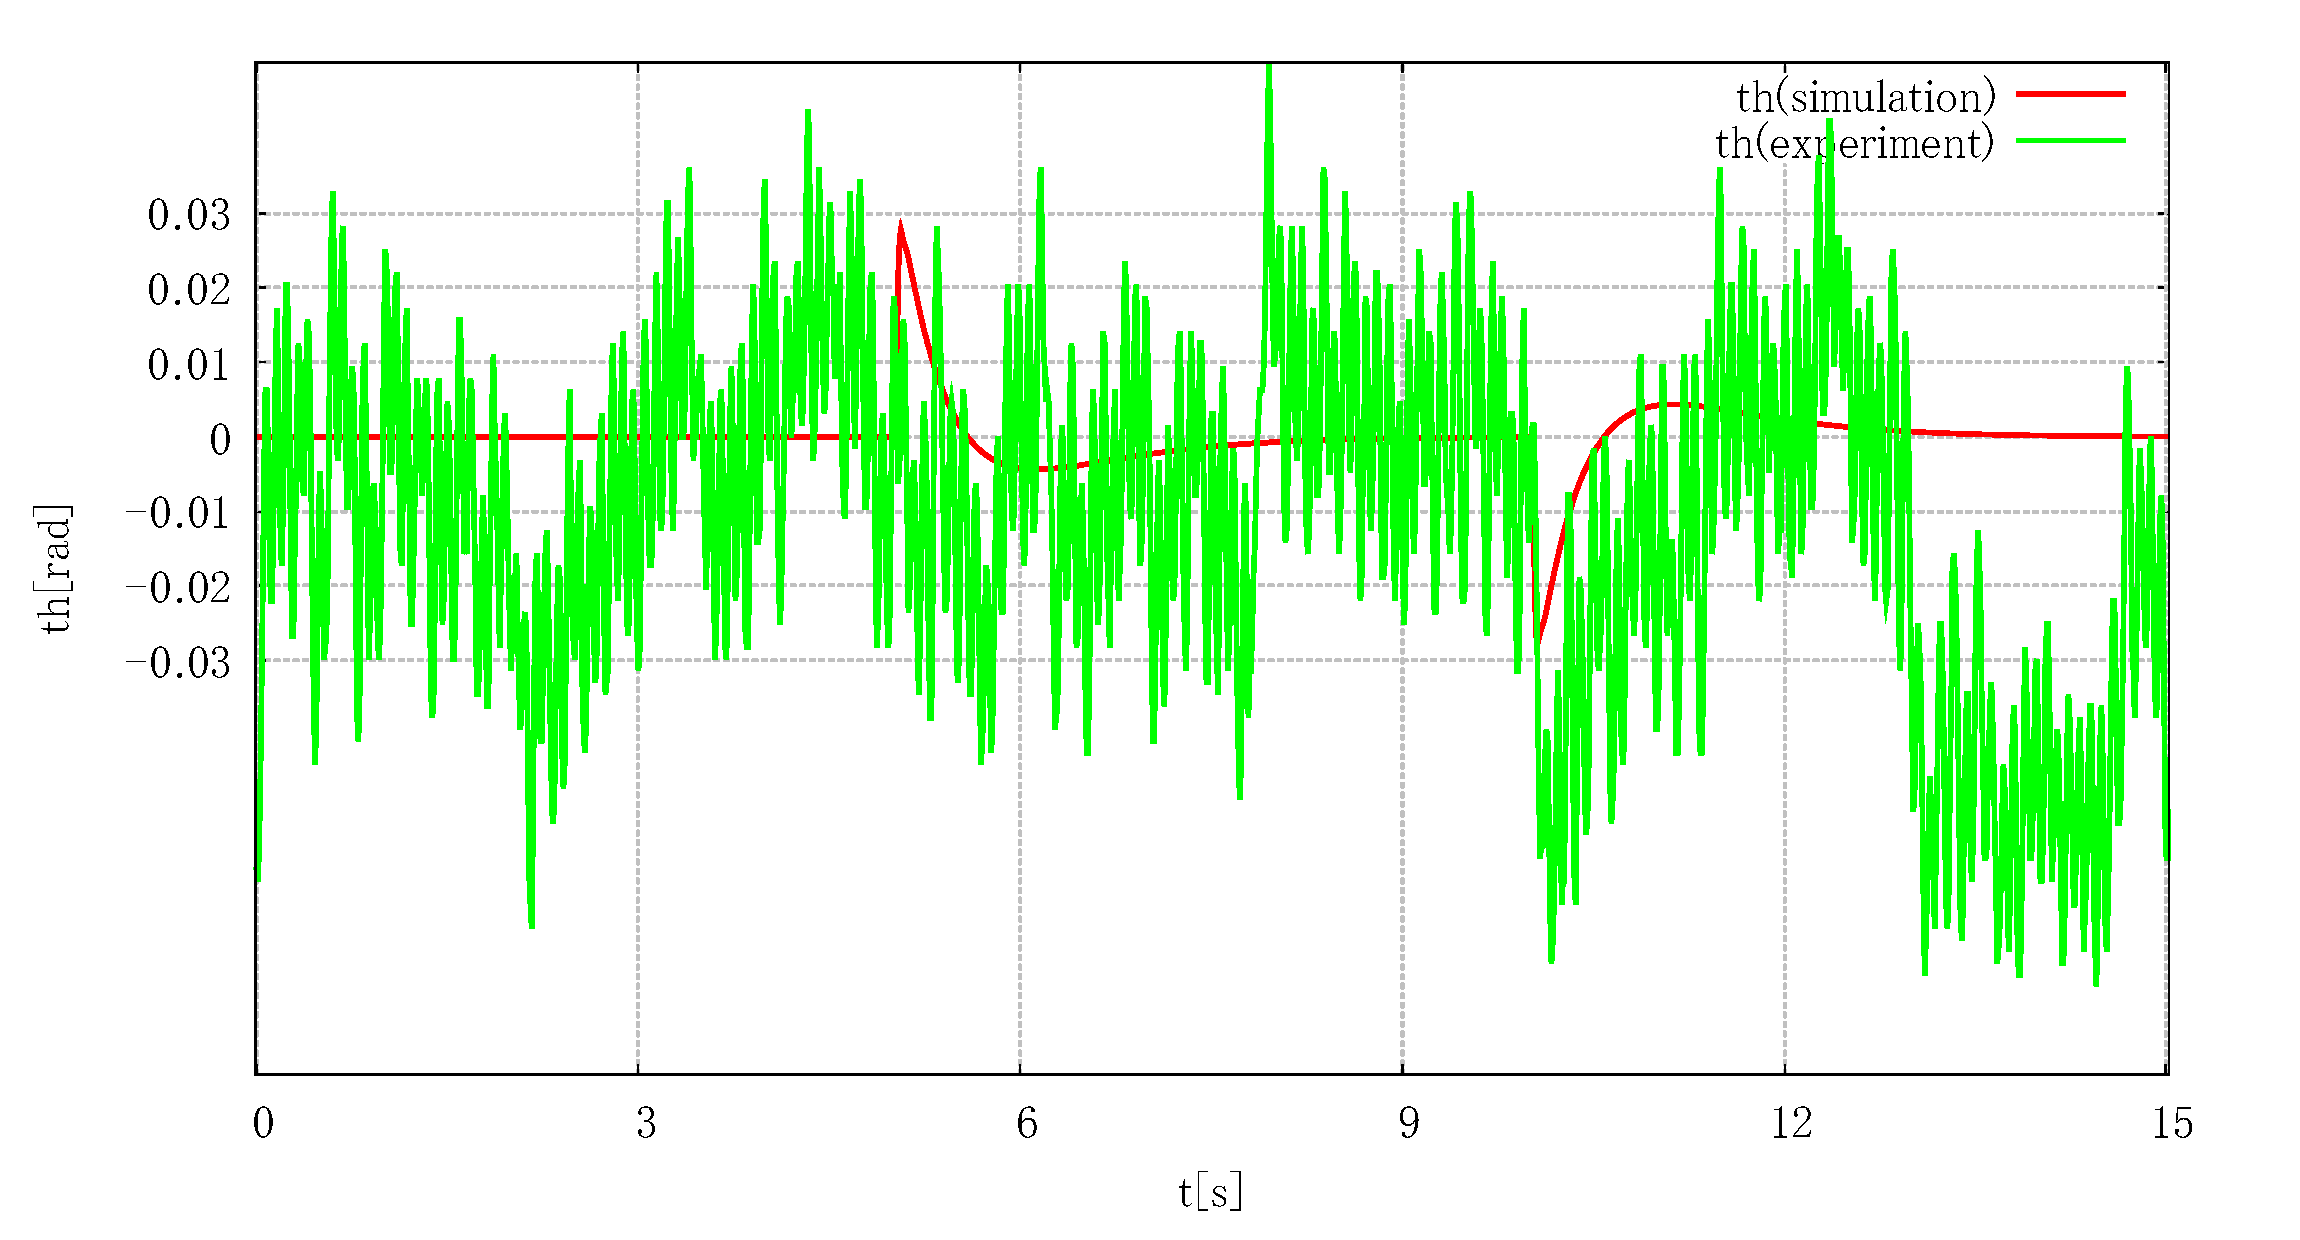
\includegraphics[width=0.4\linewidth]{gazo/experiment_Q56obs60dt10TH.eps}
		\caption{比較結果その11(左図がr,右図が$\theta$)}
		\label{image:sono11}
	\end{figure}
	\begin{figure}[H]
		\centering
		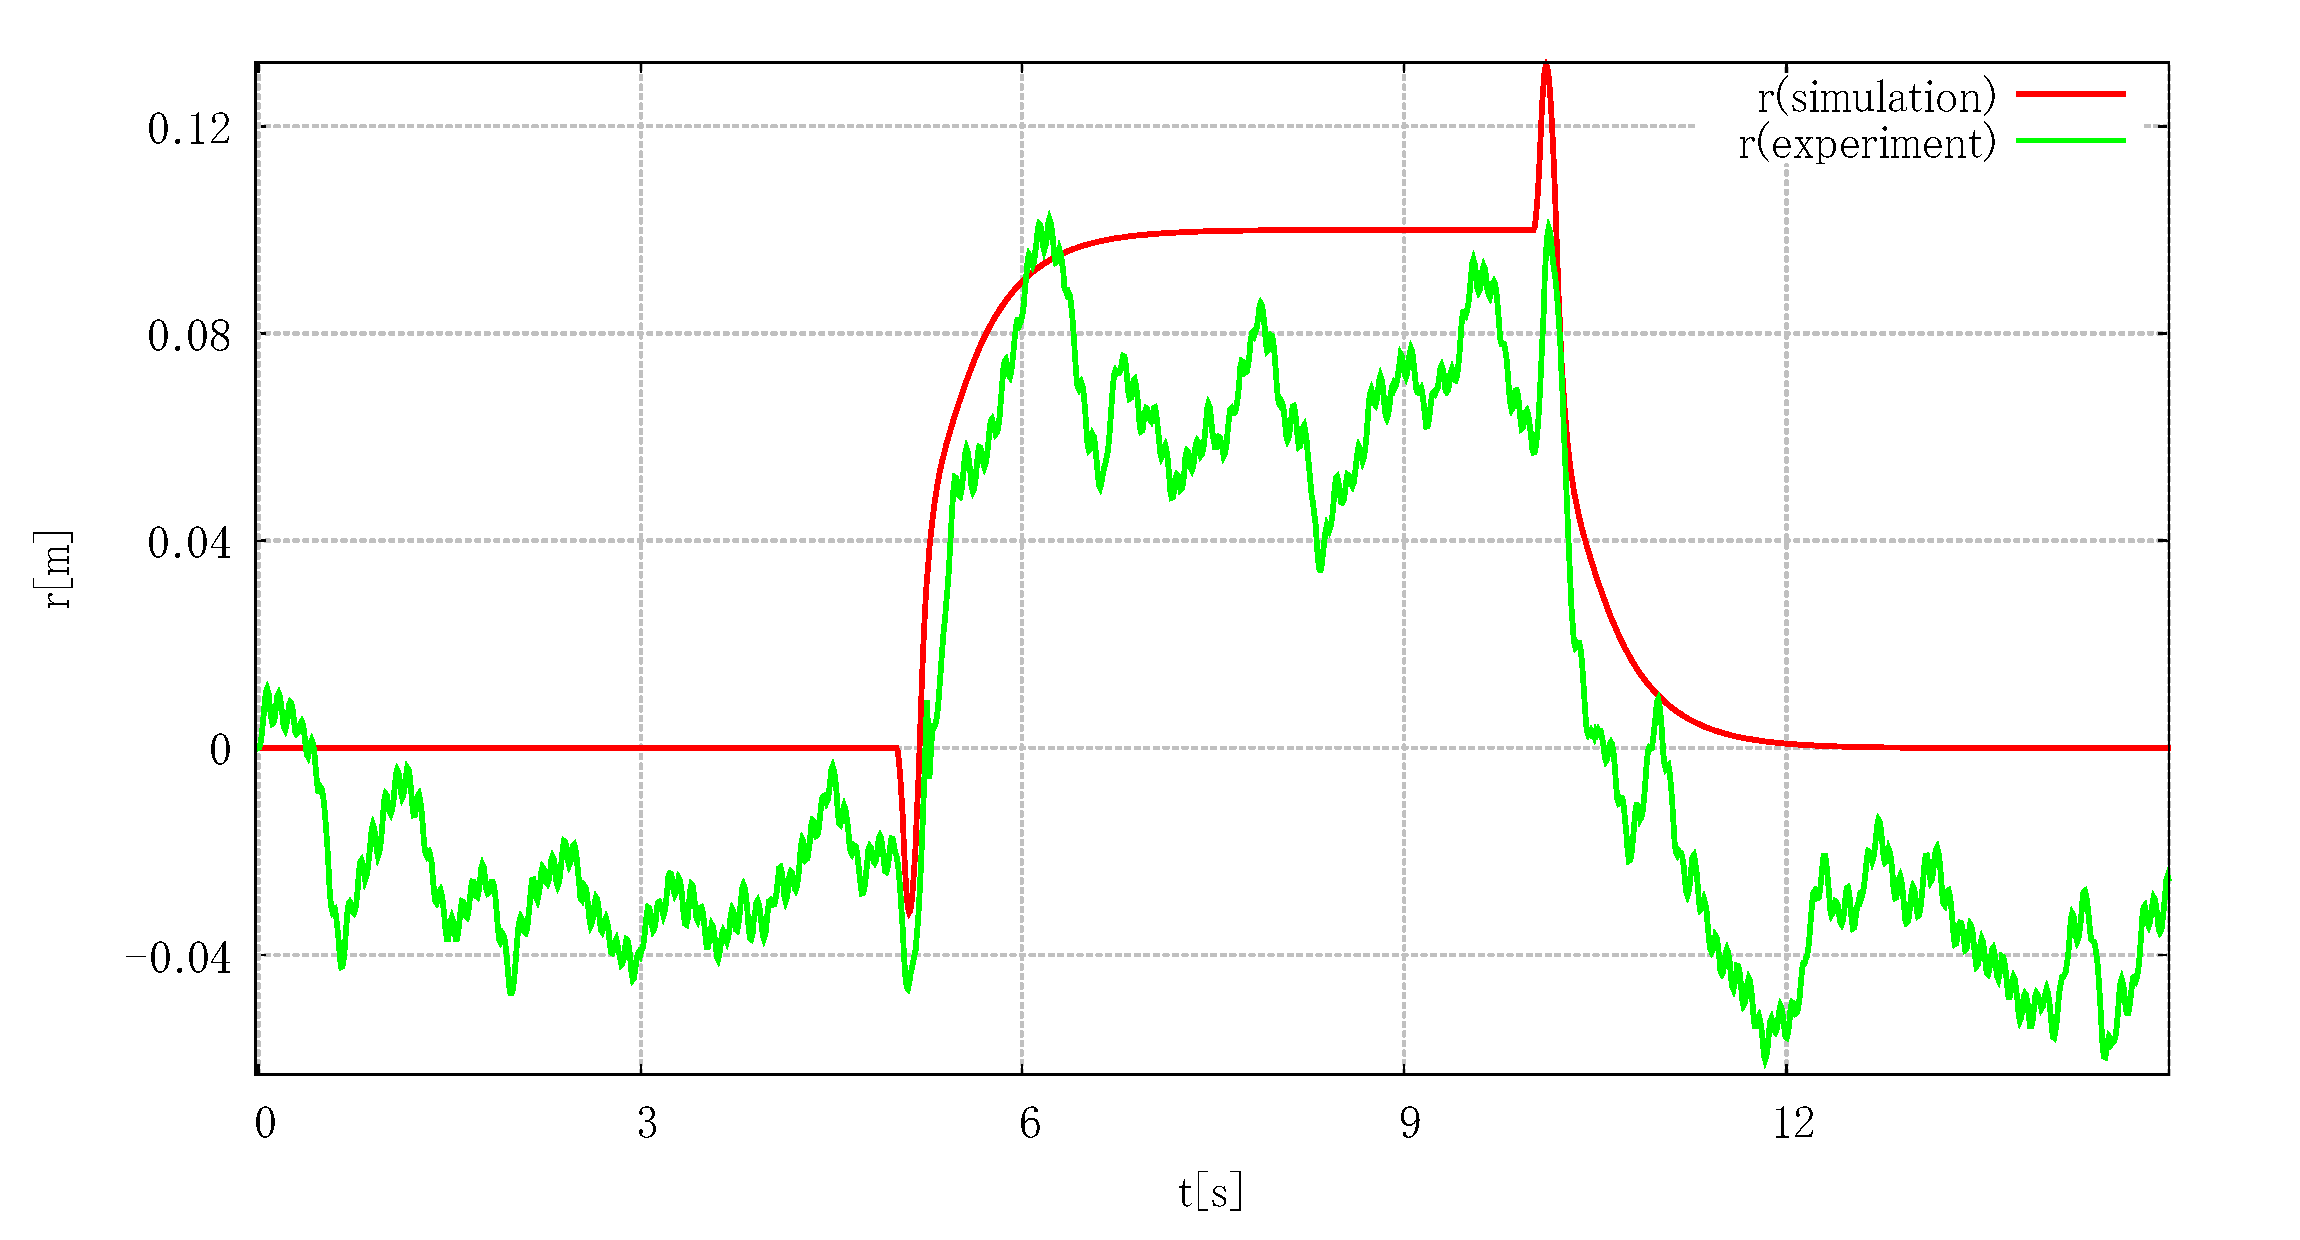
\includegraphics[width=0.4\linewidth]{gazo/experiment_Q65obs60dt10R.eps}
		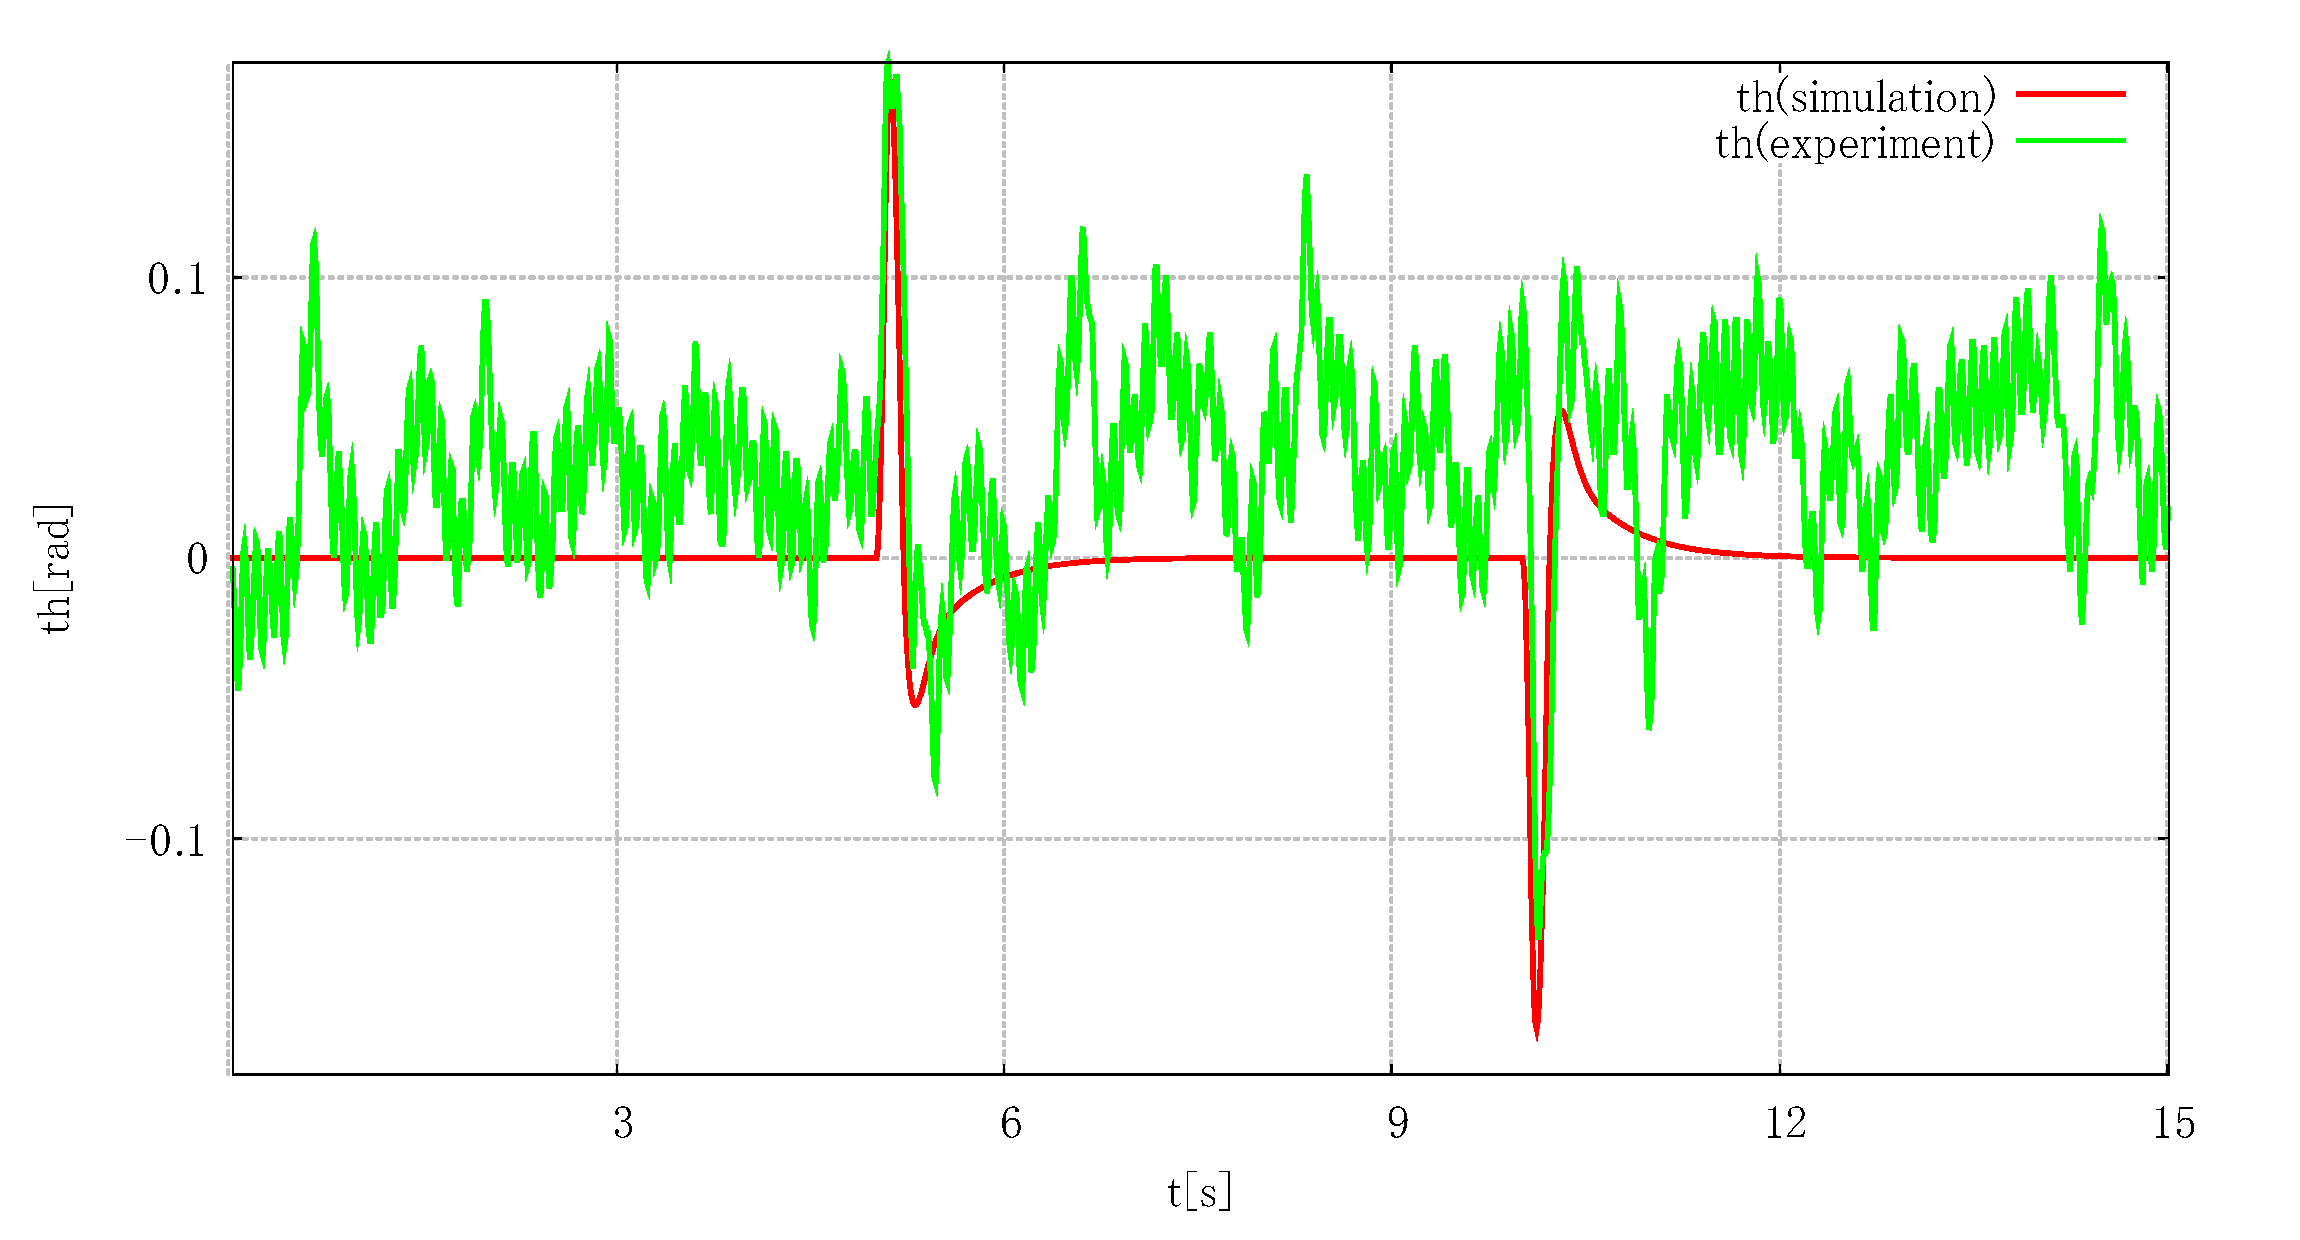
\includegraphics[width=0.4\linewidth]{gazo/experiment_Q65obs60dt10TH.eps}
		\caption{比較結果その12(左図がr,右図が$\theta$)}
		\label{image:sono12}
	\end{figure}
	以上を見てみるとすべての図においてノイズがひどいが、比較的シミュレーション結果と一致している図とまったく一致していない図があるのが分かる。
	前者に当てはまる図は図\ref{image:sono1}、図\ref{image:sono3}、図\ref{image:sono4}、図\ref{image:sono6}
	、図\ref{image:sono7}、図\ref{image:sono9}、図\ref{image:sono12}。後者に当てはまる図は、
	図\ref{image:sono2}、図\ref{image:sono5}、図\ref{image:sono8}、図\ref{image:sono11}である。
	後者に共通する特徴は重み行列が$\rm{diag}(1E5,1E6,1,1)$となっている点である。
	このようにしたときの特徴としてはシミュレーションの章でも述べたが、大きくした成分に対応する状態の応答がよくなるというものであった。
	つまり、この重み行列のとき$\theta$の応答がよくなりるはずである。
	だが、実際の図を見てみると$\theta$の応答はシミュレーションと比較しても一致しているとは言えない。
	また、$r$に関しては図を見る限りでは目標値変更ができていないといえる。
	これは、実験で用いた倒立振子系に問題があると思われる。実験で用いた倒立振子系は安定化制御を開始すると
	振子を倒立させるためにベルトが動くので、倒立振子系自体が激しく振動する。本来であれば、倒立振子系のベルトが
	動いても振動しないように固定しておくべきだが、諸事情により固定ができない状況であったためそのままの状態で
	実験を行った。この激しい振動が実験結果に影響を及ぼしたのではないかと考えられる。
	
	

%-----------------------------------------------------------
\section{振り上げ制御及び安定化実験}
	振子を真下に配置し、そこから台車の動きだけで振子を振り上げ、
	安定化制御が可能か実験を行う。(実験項目の第三項目)
	以下にその結果とシミュレーション結果との比較を行った図を示す。

%-----------------------------------------------------------